\documentclass[accentcolor=tud1b,bibliography=totoc,listof=totoc,oneside,numbersubsubsec,type=msc,fontsize=12pt,colorback]{tudthesis}
\usepackage[utf8]{inputenc}
\usepackage[T1]{fontenc}
\usepackage[english]{babel}
\usepackage{setspace}
\onehalfspacing
\usepackage{multirow}
\usepackage[german=quotes]{csquotes}
\usepackage{psfrag}
\usepackage[style=numeric,firstinits=true,backend=bibtex,maxbibnames=99,sorting=nty]{biblatex}
\bibliography{bibliography}
\usepackage{tikz}
\usetikzlibrary{shapes,shapes.geometric,automata,positioning,arrows}
\usepackage{pgfplots}
\pgfplotsset{compat=newest}
\usetikzlibrary{patterns}
\usepackage{url}
\usepackage{amsmath}
\usepackage{amsthm}
\usepackage{graphicx}
\usepackage{placeins}
\usepackage{breakurl}
\usepackage[ruled,linesnumbered,commentsnumbered]{algorithm2e}
\usepackage{listings}
\renewcommand{\lstlistlistingname}{List of Code Snippets}
\usepackage{booktabs}
\usepackage{tabularx}
\usepackage{enumitem}
\usepackage{bm}
\usepackage{perpage}
\MakePerPage{footnote}
\usepackage{caption}
\usepackage{subcaption}
\usepackage{pgf-umlcd}
\usepackage{gnuplottex}
\usepackage{multirow}

\lstset{
    numbers = left, 
    numberstyle = \scriptsize\bfseries, 
    stepnumber = 1, 
    numbersep = 5pt,
    tabsize = 4,
    literate = {\ \ }{{\ }}1,
    keywordstyle = \bfseries,
    basicstyle = \ttfamily,
    frame = tb
}

\begin{document}

\thesistitle{Auto-Scaling Techniques for Spark Streaming}{}
\author{Seyedmajid Azimi Gehraz}
\birthplace{Iran}
\referee{Prof. Dr. rer. nat. Carsten Binnig}{Dr. Thomas Heinze}{}
\department{Fachbereich Informatik}
\group{Data Management}
\dateofexam{\today}{\today}

\makethesistitle
\affidavit{Seyedmajid Azimi Gehraz}

\pagenumbering{Roman}

\tableofcontents
\clearpage
\listoffigures
\clearpage
\listoftables
\clearpage
\lstlistoflistings
\clearpage
\listofalgorithms
\addcontentsline{toc}{chapter}{List of Algorithms}
\clearpage
\newcounter{romanpagenumbers}
\setcounter{romanpagenumbers}{\value{page}}

\pagenumbering{arabic}

\chapter{Abstract}
\chapter{Problem Definition}
\label{prob-def}
\section{Introduction}
Cloud computing has been on rise over the last decade. Parts of this popularity is due to its inherent features. It lets application developers to run their applications on virtual infrastructure. Virtual infrastructure lays the foundation of on-demand infrastructure. Developers acquire and release resources as required by workload. Examples of cloud providers are Amazon AWS~\cite{aws}, Microsoft Azure~\cite{azure} and Google Cloud~\cite{gc}. Today's cloud infrastructure is widely used by many customers for different purposes such as batch processing, serving static content, storage servers and alike.

As cloud environment brings up \emph{elasticity}~\cite{Roman:2013}, it also introduces a new set of challenges and problems. Modern applications face fluctuating workloads. Typically, if a workload is \emph{predictable}, resources are allocated ahead of time before load-spike starts. However, in many other scenarios predicting even near future workload is a not so easy task. Even though running an application in cloud environments helps to overcome a long standing problem of \emph{over-provisioning}, low utilization is still one of the major problems of cloud applications. This has been confirmed by multiple studies~\cite{Delimitrou:2014}~\cite{Reiss:2012}.

The root of the problem is originated from the fact that, most developers do not have enough insight about bottom and peak workload of their application. Thus, they fail to define an effective scaling strategy. Therefore, they end up with conservative strategies which in turn leads to low utilization. Hence, we need a system that automates the process of resource allocation. Auto-Scaling has been well studied in the context of web application.~\cite{Hasan2012IntegratedAA}~\cite{Dutreilh2010}~\cite{Herbst:2013} are just a few examples. Chapter~\ref{related} explores more techniques and strategies.

\section{Objectives of Auto-Scaling Systems}
The ultimate goal of an Auto-Scaling system is to automate the process of acquiring and releasing \emph{resources} in order to minimize the \emph{cost} with minimum violation of \emph{service level objectives} (SLO). The definition of \emph{resource} depends on the context. As an example, for a stateless web applications it means virtual machines or containers that run web server software. For an Auto-Scaling system to adjust required resources, it shall consider different aspects of application and environment. Additionally, the term \emph{cost} is also defined in the context. As an example, it might mean monetary cost or just numerical value of resources. SLOs are predefined rules that shall not be violated during application runtime and are also defined in the context of application.

\section{Auto-Scaling in Data Stream Processing Systems}
\emph{Data Stream Processing Systems} are data processing systems that process \emph{unbounded} stream of data unlike their \emph{batch-oriented} counterparts. With the ever increasing adoption of IoT applications, it is critical to design stream processing systems that handles the incoming messages with high throughput and low latency. With static workloads, these problems could be solved by dominating stream processing systems like Apache Spark~\cite{spark}, Apache Storm~\cite{Storm} and Apache Flink~\cite{flink}. However, the problem of low utilization also applies for stream processing systems as well. This leads us to a new generation of stream processing systems called \emph{Elastic Data Processing Systems} that adopts elasticity concepts to stream processing system.

Prior to this thesis a number of studies have been performed on elastic stream processing system. \cite{CastroFernandez:2013},~\cite{Heinze:2014} are just a few samples. One of the dominating stream processing systems is Apache Spark which support both batch and stream processing. In order to support both workloads, Apache Spark has a unique architecture that partitions the input workload into predefined window of batches -- an architecture known as micro batching. With this common architecture as a foundation, number of interesting challenges arise that need to be considered for elastic workloads.

This thesis will focus on dynamic resource allocation in the context of Apache Spark. An extensible framework will be developed based on a prior work by \textcite{Michal:2017}. This thesis will extend the existing prototype and implement multiple Auto-Scaling techniques for Apache Spark Streaming and will evaluate these techniques using real-world workloads. The ultimate goal is to identify how the architecture of Spark Streaming influences the performance of the different Auto-Scaling techniques.

\section{Summary}
As mentioned this thesis will focus on dynamic resource allocation in the context of Apache Spark. The thesis is organized as follows. Chapter~\ref{intro-auto-scale} introduces and explains basics of Auto-Scaling techniques. Chapter~\ref{spark} introduces the architecture of Apache Spark Streaming. Chapter~\ref{design} explains structure and design considerations of this thesis. Chapter~\ref{detail} discusses implementation details and challenges faced during implementation. Chapter~\ref{eval} evaluates the implementation under different workloads. Chapter~\ref{related} includes discussion of prior and related work. Finally, chapter~\ref{conc} concludes.
\chapter{Introduction to Auto-Scaling}
\label{intro-auto-scale}


\begin{itemize}
    \item \emph{Service Level Objective} (SLO): Each application has its own set of predefined rules that shall not be violated during the process of acquiring and releasing resources. These rules typically context and application dependent. For example for web applications, one may define maximum round-trip latency that a user should wait until her request is fulfilled. 
    \item \emph{Unit of allocation}
\end{itemize}
\chapter{Apache Spark and Spark Streaming}
\label{spark}

\section{Introduction}
\label{sp:intro}

Apache Spark~\cite{spark} is a general purpose data processing framework that supports wide range of applications from \emph{batch} processing, \emph{stream} processing, \emph{graph} processing to \emph{machine learning}, etc. In this chapter the architecture of Apache Spark and Spark Streaming -- as one of its sub projects -- will be explored and discussed. Throughout the chapter, minor examples will also be presented to further simplify the concepts. This chapter is organized as follows. Section~\ref{sp:basics} explains the basic concepts of Apache Spark. Then, section~\ref{sp:rdd} explains \emph{Resilient Distributed Datasets} (RDDs) which is the most integral component of the Apache Spark. Section~\ref{sp:dstream} explains \emph{Discretized Streams} (DStreams) as the fundamental building block for data stream processing applications. Finally, section~\ref{sp:conc} concludes this chapter.

\section{Basic Concepts}
\label{sp:basics}

Map-Reduce~\cite{Dean:2004} and its derivative projects have been widely used by \emph{data-oriented} applications to process and crunch huge datasets over last the decade. In traditional Map-Reduce environments, developers typically create \emph{acyclic} data flow graphs to process input data. However, as confirmed by \textcite{Zaharia:2010}, there are two categories of applications that are not well suited for this architecture.
\begin{itemize}
    \item \textbf{Iterative Jobs} Many machine learning applications process the same input \emph{iteratively}. In traditional model, each iteration should be defined as a separate MapReduce job. While this is feasible, but for each job, input data has to be loaded from disk which leads to serious performance issues.
    \item \textbf{Interactive Analysis} MapReduce derivative projects like Hive~\cite{hive} and Pig~\cite{pig} have been extensively used to run SQL queries on top of massive datasets. Whenever a user submits different queries over the same dataset, the ideal solution would be to load all datasets into memory once and then execute different queries on top of it. However, with traditional model of execution each query shall be defined as a separate job which reads input data from disk.
\end{itemize}
Apache spark has been designed from ground up to resolve these issues. It provides a large stack of tools to facilitate processing large datasets. Figure~\ref{fig:spark-eco} depicts tools provided by Spark.
\begin{figure}[h]
    \centering
    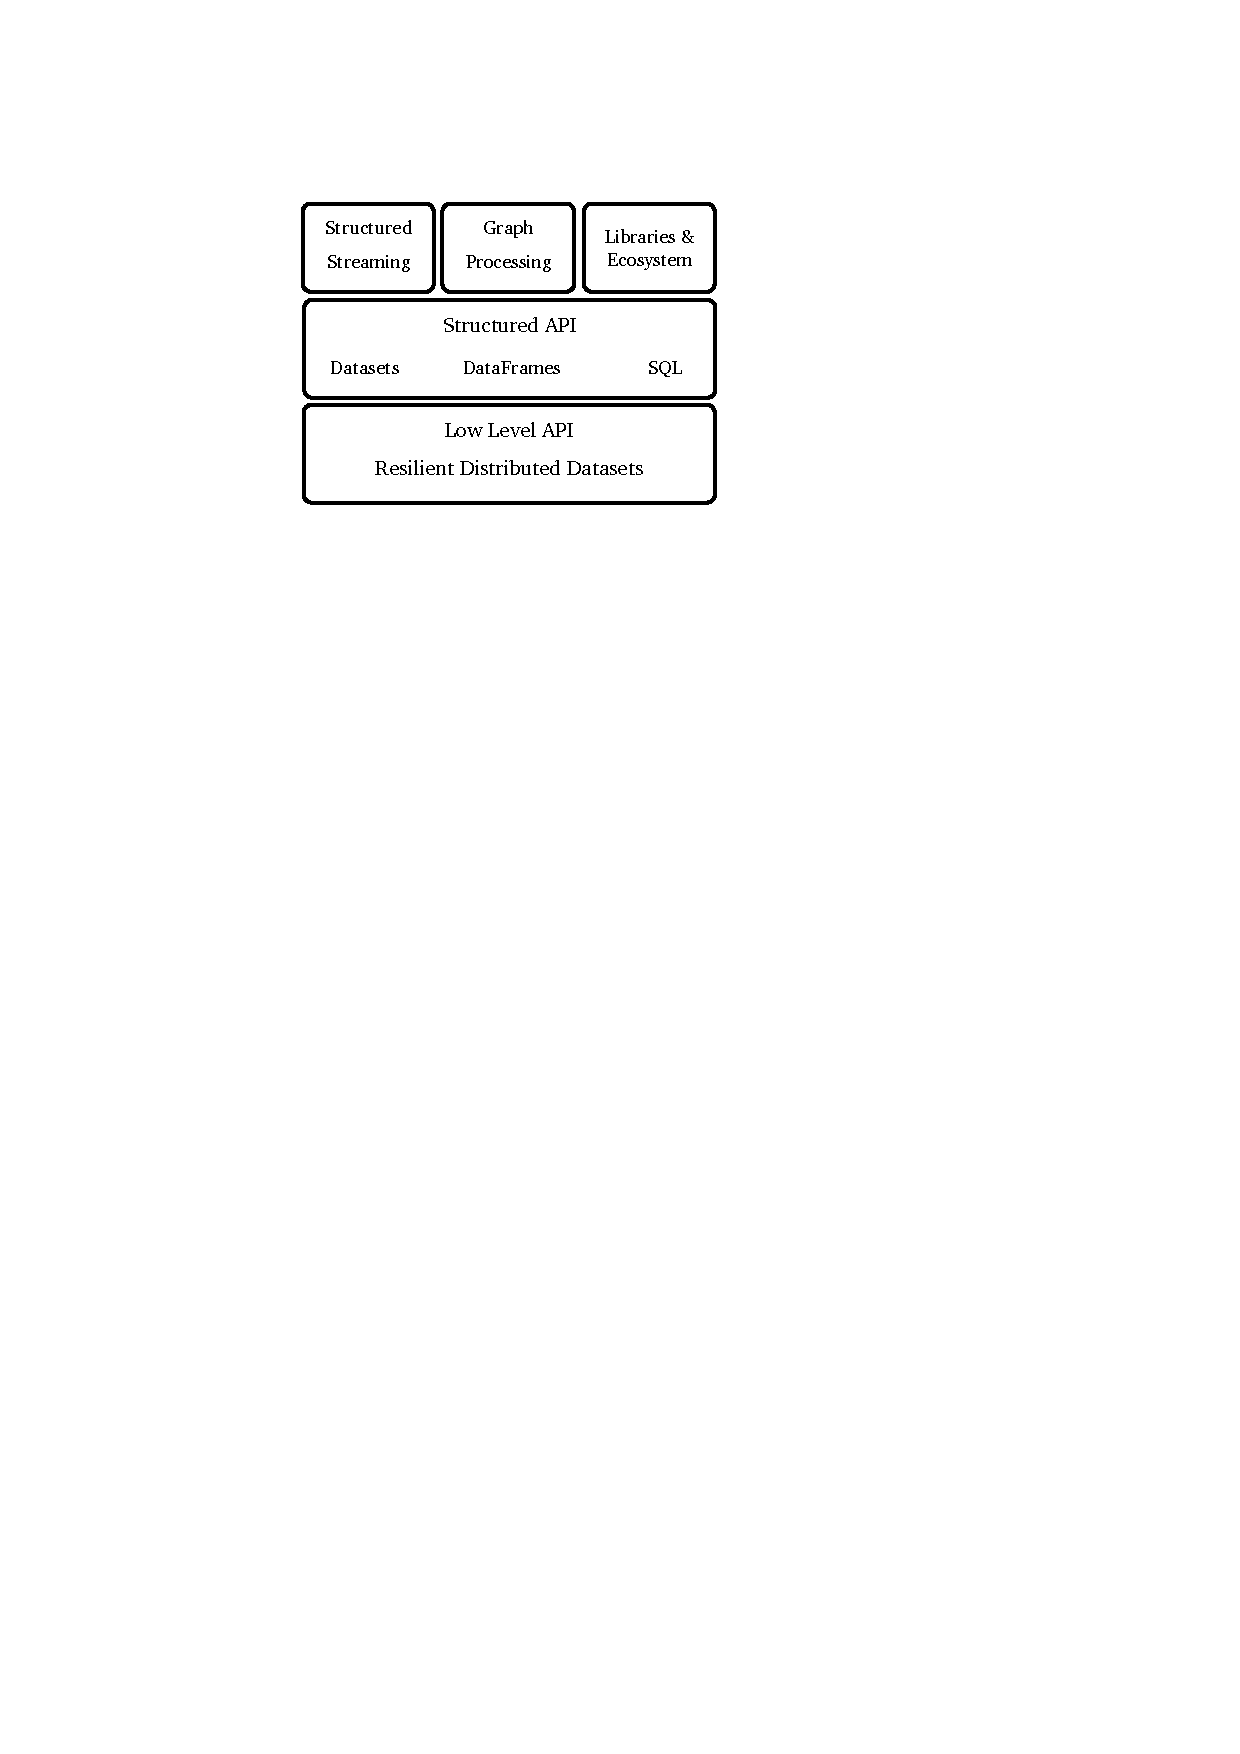
\includegraphics[clip,trim=5cm 21.1cm 8.7cm 3.4cm]{spark-eco.pdf}
    \caption{Apache Spark Stack}
    \label{fig:spark-eco}
\end{figure}

\subsection{Spark Runtime Architecture}
\label{sp:run}

Any Spark application consists of multiple components at runtime. The following lists the relevant components from a high level point of view.
\begin{description}[leftmargin=0pt]
    \item[Driver Process] It is the core component of every Spark application. It is a single process and runs on one of the nodes in the cluster. It maintains all the critical information such as user's program, input files, output files and data flow of the application. The driver process should run during the runtime the of the application. In case driver process fails, the whole application is considered as \emph{dead} and should be restarted by any \emph{fault-tolerance} mechanism available in the cluster.
    \item[Distributed File System] It provides a shared file system accessible by any node in the cluster. There is no limitation on type of the file system but typically \emph{Hadoop Distributed File System} (HDFS)~\cite{hadoop} is used.
    \item[Worker Processes] A collection of worker processes known as \emph{executors} that run on cluster nodes. Executors run user defined code. During the runtime of the application each worker consume any number of input records, processes it based on user defined code and emits any number of output records. Similar to driver process, liveness of the worker processes shall by monitored. However, the role of worker processes are not as critical as driver process, even though they may fail for any reason. Workers have access to load/store data files from/to distributed file system or local memory of the machine. During lifetime of the application, status of the workers will be reported to driver process.
    \item[User Defined Code] Provided by user and caries the main logic of the application.
\end{description}
Figure~\ref{fig:spark-runtime}\footnote{The figure has been partially taken from~\textcite{Zaharia:2012}} depicts coarse grained architecture of a Spark application and table~\ref{tab:spark-runtime} summarizes these components.
\begin{figure}[h]
    \centering
    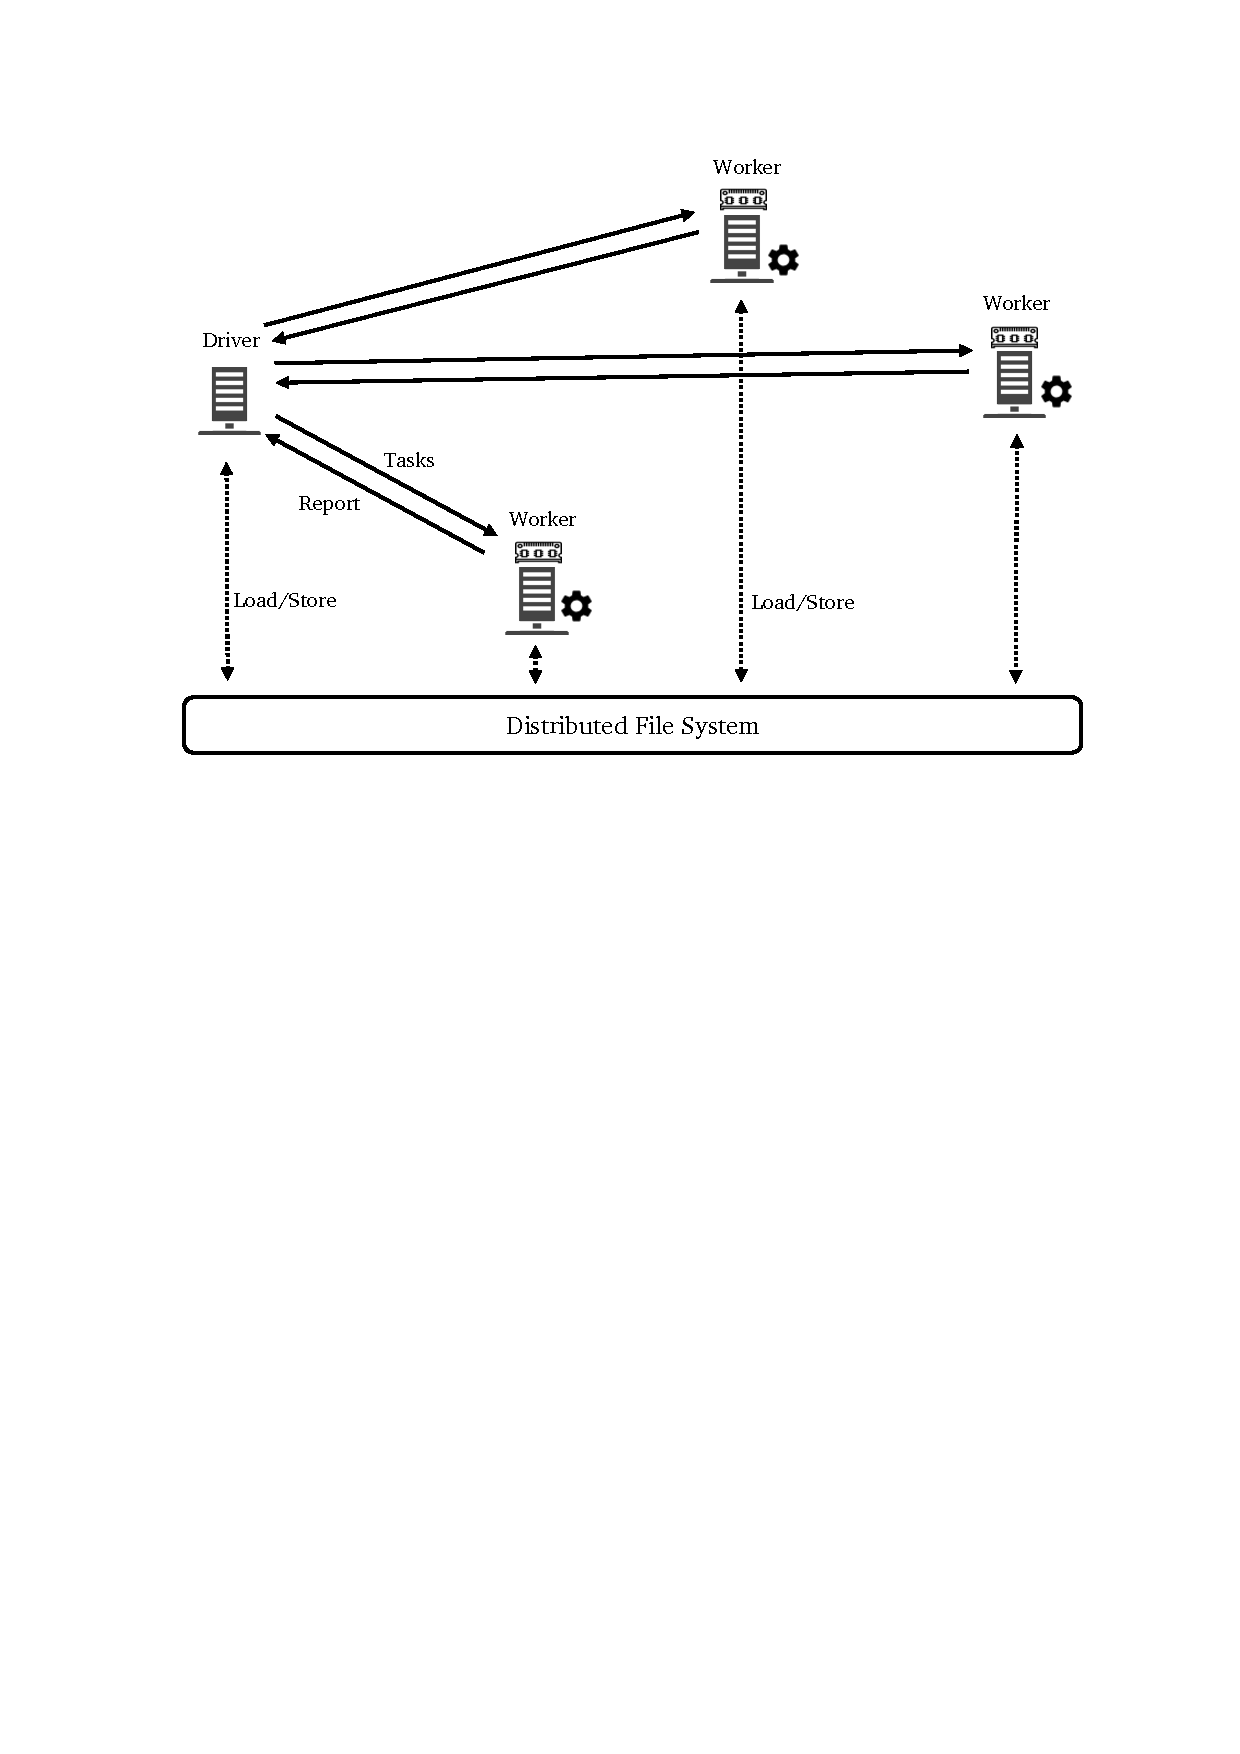
\includegraphics[clip,trim=3cm 16.8cm 2.5cm 2.5cm]{spark-high.pdf}
    \caption{Architecture of Spark Runtime}
    \label{fig:spark-runtime}
\end{figure}
\begin{table*}[ht]
    \begin{tabularx}{\textwidth}{lX}
        \toprule
        \textbf{Component} & \textbf{Description}\\
        \midrule
        Driver & Maintains all relevant information -- including user defined code -- to process input data and produce output.\\
        Distributed File System & Provides shared file system accessible by all nodes in cluster.\\
        Worker Process & Workforce of the cluster. Gets necessary information from driver and executes user defined code.\\
        User Defined Code & Caries the main application logic.\\
        \bottomrule
    \end{tabularx}
    \centering
    \caption{Summary of Spark Runtime Components}
    \label{tab:spark-runtime}
\end{table*}

\subsection{Spark Cluster Manager}
\label{sp:cluster}

Section~\ref{sp:run} described the coarse grained architecture of Spark. However, from a more fine grained point of view, there is missing component known as \emph{Cluster Manager}. Cluster Manager controls the \emph{assignment} of executors to cluster nodes. It monitors liveness of executors during lifetime of the Spark application. \emph{Spark Session} is the entry point for all Spark applications and has the responsibility to communicate with Cluster Manager to distribute tasks and collect task progress reports from executors. It also distributes user defined code on Worker nodes. Figure~\ref{fig:spark-cluster}\footnote{The figure has been partially taken from~\textcite{spark-guide}} illustrates the role of Cluster Manager in Spark.
\begin{figure}[h]
    \centering
    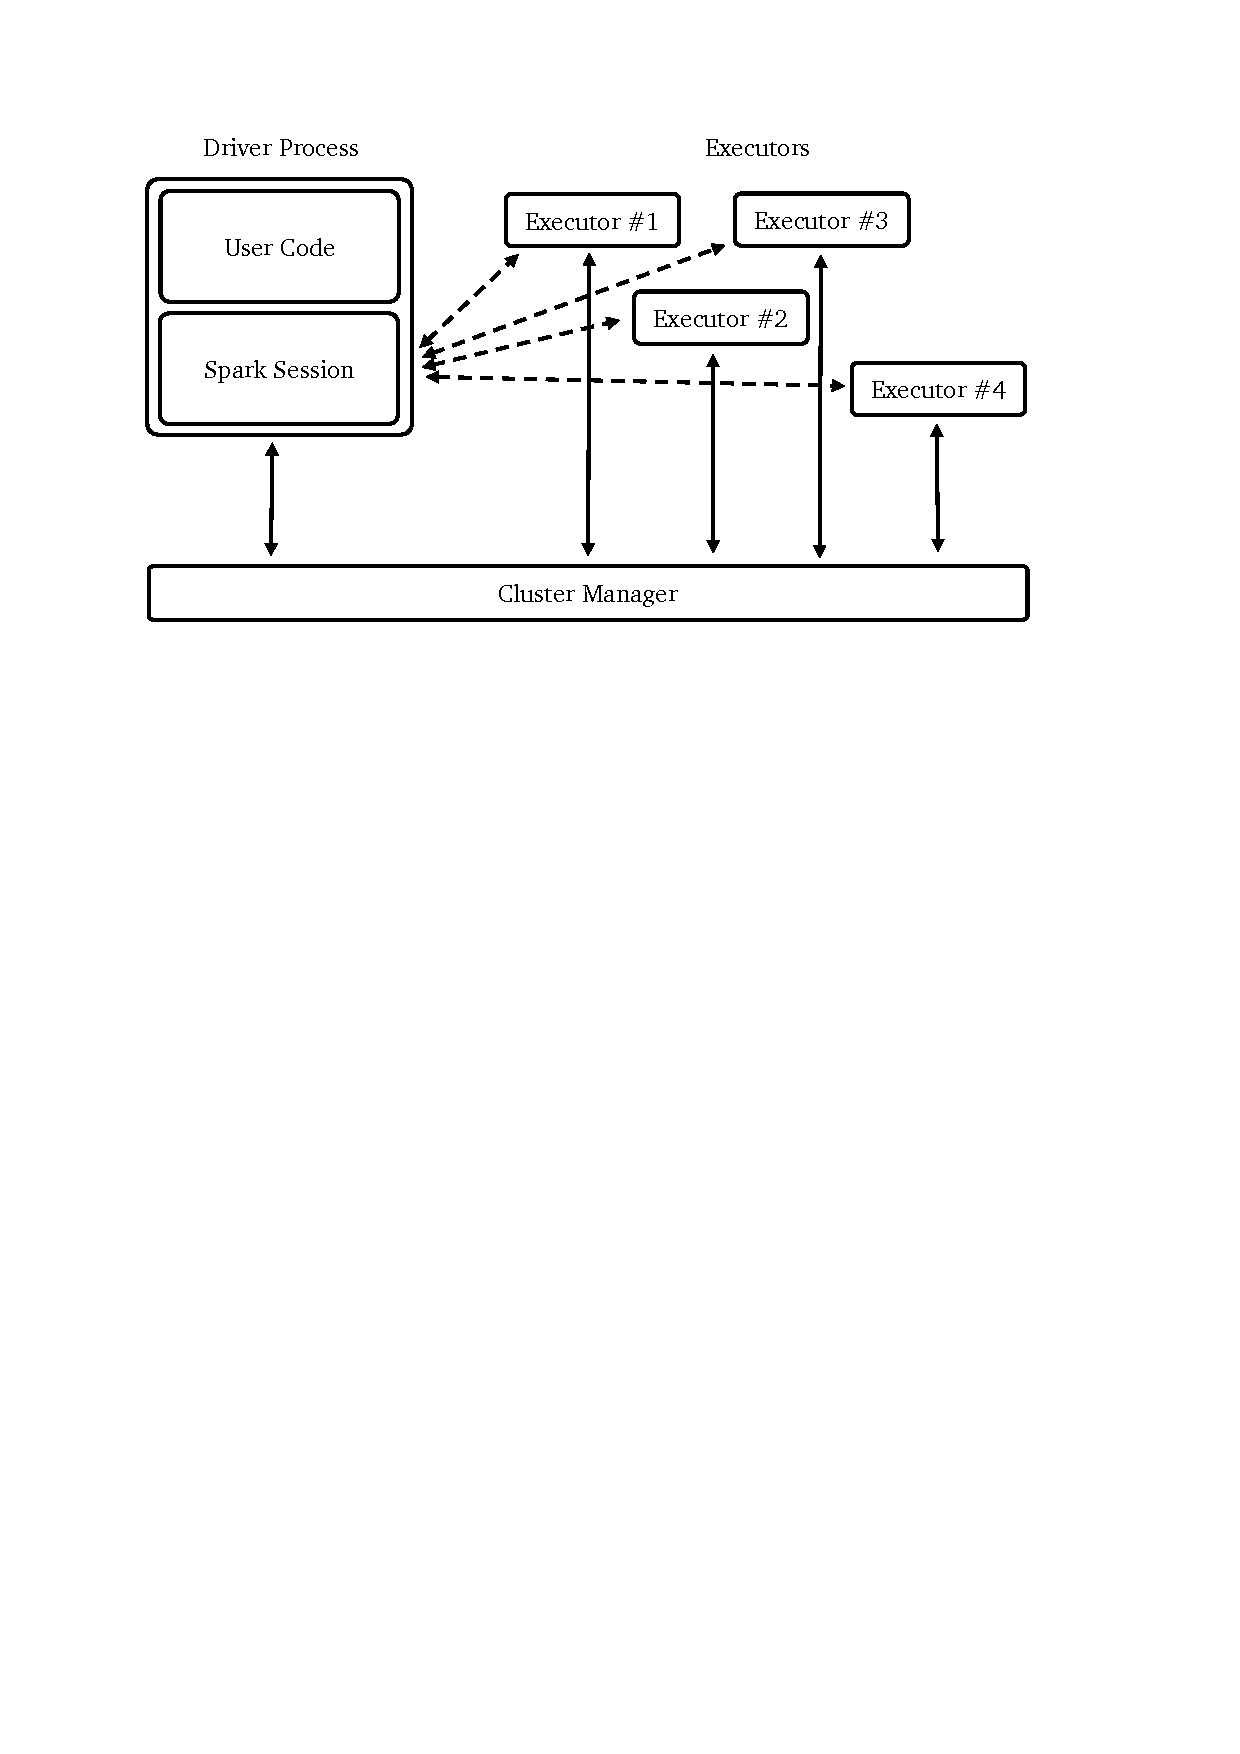
\includegraphics[clip,trim=2.4cm 19cm 3.5cm 2cm]{spark-cluster.pdf}
    \caption[Architecture of Spark Cluster Manager]{Architecture of Spark Cluster Manager}
    \label{fig:spark-cluster}
\end{figure}

Note that, the term \emph{executor} is a conceptual term and implementation details may differ among different resource managers. Spark supports multiple Cluster Manager implementations. The following describes the most prominent implementations. It shall be noted that this list is a growing over time due to Spark's pluggable resource manager architecture. Table~\ref{tab:spark-cluster} summarizes available Cluster Manager architectures.
\begin{table*}[h]
    \begin{tabularx}{\textwidth}{lX}
        \toprule
        \textbf{Cluster Manager} & \textbf{Description}\\
        \midrule
        Apache YARN & Hierarchical failure detection. Global Resource Manager monitors local Node Managers and Application Masters. Backup Resource Managers monitor global Resource Manager. Node Managers monitor local containers.\\
        Apache Mesos & Hierarchical failure detection. Mesos Master monitors Mesos Slaves and Framework Schedulers. Backup masters monitor Mesos Master. Mesos Slaves monitor local workers.\\
        Spark Standalone & Spark Master monitors Driver program and Spark Slaves. Backup master monitor Spark Master. Spark Slaves monitor local executors.\\
        \bottomrule
    \end{tabularx}
    \centering
    \caption{Summary of Spark Cluster Managers}
    \label{tab:spark-cluster}
\end{table*}
\begin{description}[leftmargin=0pt]
    \item [Apache YARN] It is referred as \emph{Yet Another Resource Negotiator}~\cite{Vavilapalli:2013} and is the default resource manager for modern Hadoop workloads. It has a master-slave architecture and consists of a single global \emph{Resource Manager} -- most probably accompanied by a backup as well --  and several \emph{Node Managers} that run on each worker node. The concept of executor is implemented as \emph{containers} in YARN. Each container can hold a specific amount of node's processing power (CPU, RAM, Network, etc.). In YARN, any application is modeled with two components. First, \emph{Application Master} that maintains the necessary information to run the application -- Spark driver process in this case and second, several \emph{Workers} that run the user defined code. Both Application Master and Workers are executed in the context of YARN containers. 
    
    Fault-tolerance is provided at multiple levels. First, several backup nodes monitor the master resource manager via Zookeeper. In case master resource manager fails, one of the backup masters takes over the responsibility. Second, Applications Master reports its status to the global resource manager. In case, application master fails, the global resource manager launches a new Application Master on another node. Third, Workers provide different progress reports to Application Master and Node Managers. In case any Worker container fails, a new container will be allocated and the old one will be killed by the local Node Manager.
    \item [Apache Mesos] It is another dominant cluster scheduler for Spark~\cite{Hindman:2011}. It is a master-slave resource manager. A global resource manager -- known as \emph{Mesos Master} -- has cluster level view. On each node runs a single \emph{Mesos Slave} process. Mesos has a pluggable architecture for different class of application schedulers. That is, a single cluster can run a mixture of Spark, MPI, etc. jobs with different priority for each application type. Each \emph{Framework Scheduler} handles corresponding jobs. For example, Spark scheduler, maintains multiple driver processes or MPI scheduler maintains multiple MPI applications. Free resources on each Mesos Slave are represented as empty \emph{slots} -- very much like containers in YARN -- and are allocated to one of the currently running jobs.
    
    Fault-tolerance is provided by a similar hierarchical approach like YARN. Mesos Master is monitored by several backups through Zookeeper. Mesos Slaves as well as Framework Schedulers are in turn monitored by Mesos Master. Each job is further monitored by corresponding Framework Scheduler. And finally, executors are monitored by Mesos Slaves. 
    \item [Spark Standalone] It is the default resource manager for Spark and will be used throughout this thesis. It also follows the master-slave model. \emph{Spark Master} is the global cluster level resource manager. On each cluster node runs a \emph{Spark Slave} process. Spark Slaves are responsible to run and monitor worker executors. It is possible to set default number of CPU cores and available memory for each executor through configuration, either \emph{statically} which is applied to all jobs or at \emph{submission} time for a specific job.
    
     Fault-tolerance is achieved by several measures. Figure~\ref{fig:spark-full}\footnote{The figure has been partially taken from~\textcite{spark-guide}} depicts fault-tolerance architecture of Spark. Similar to YARN and Mesos, a multi-level failure detection approach is exploited. Multiple backup nodes monitor the Spark Master via Zookeeper~(Case~1). Spark Slaves and Drivers are monitored by Spark Master (Case 2). Progress of each executor -- whether the assigned task is done or not -- is monitored by Driver (Case 3). Initial input and final output of the jobs are stored in a distributed replicated file system like HDFS. In case any executor fails to store its final output in DFS, it will be relaunched by Spark on another node (Case 4). Intermediate results are stored locally without any fault-tolerance in mind. However, \emph{checkpoints} -- stored on DFS -- can be used in this case to recover from executor failures (Case 4). Refer to section~\ref{sp:rdd} for more information on checkpointing process. Liveness of each executor is further monitored by corresponding local Spark Slave process (Case 5)
     \begin{figure}[ht]
         \centering
         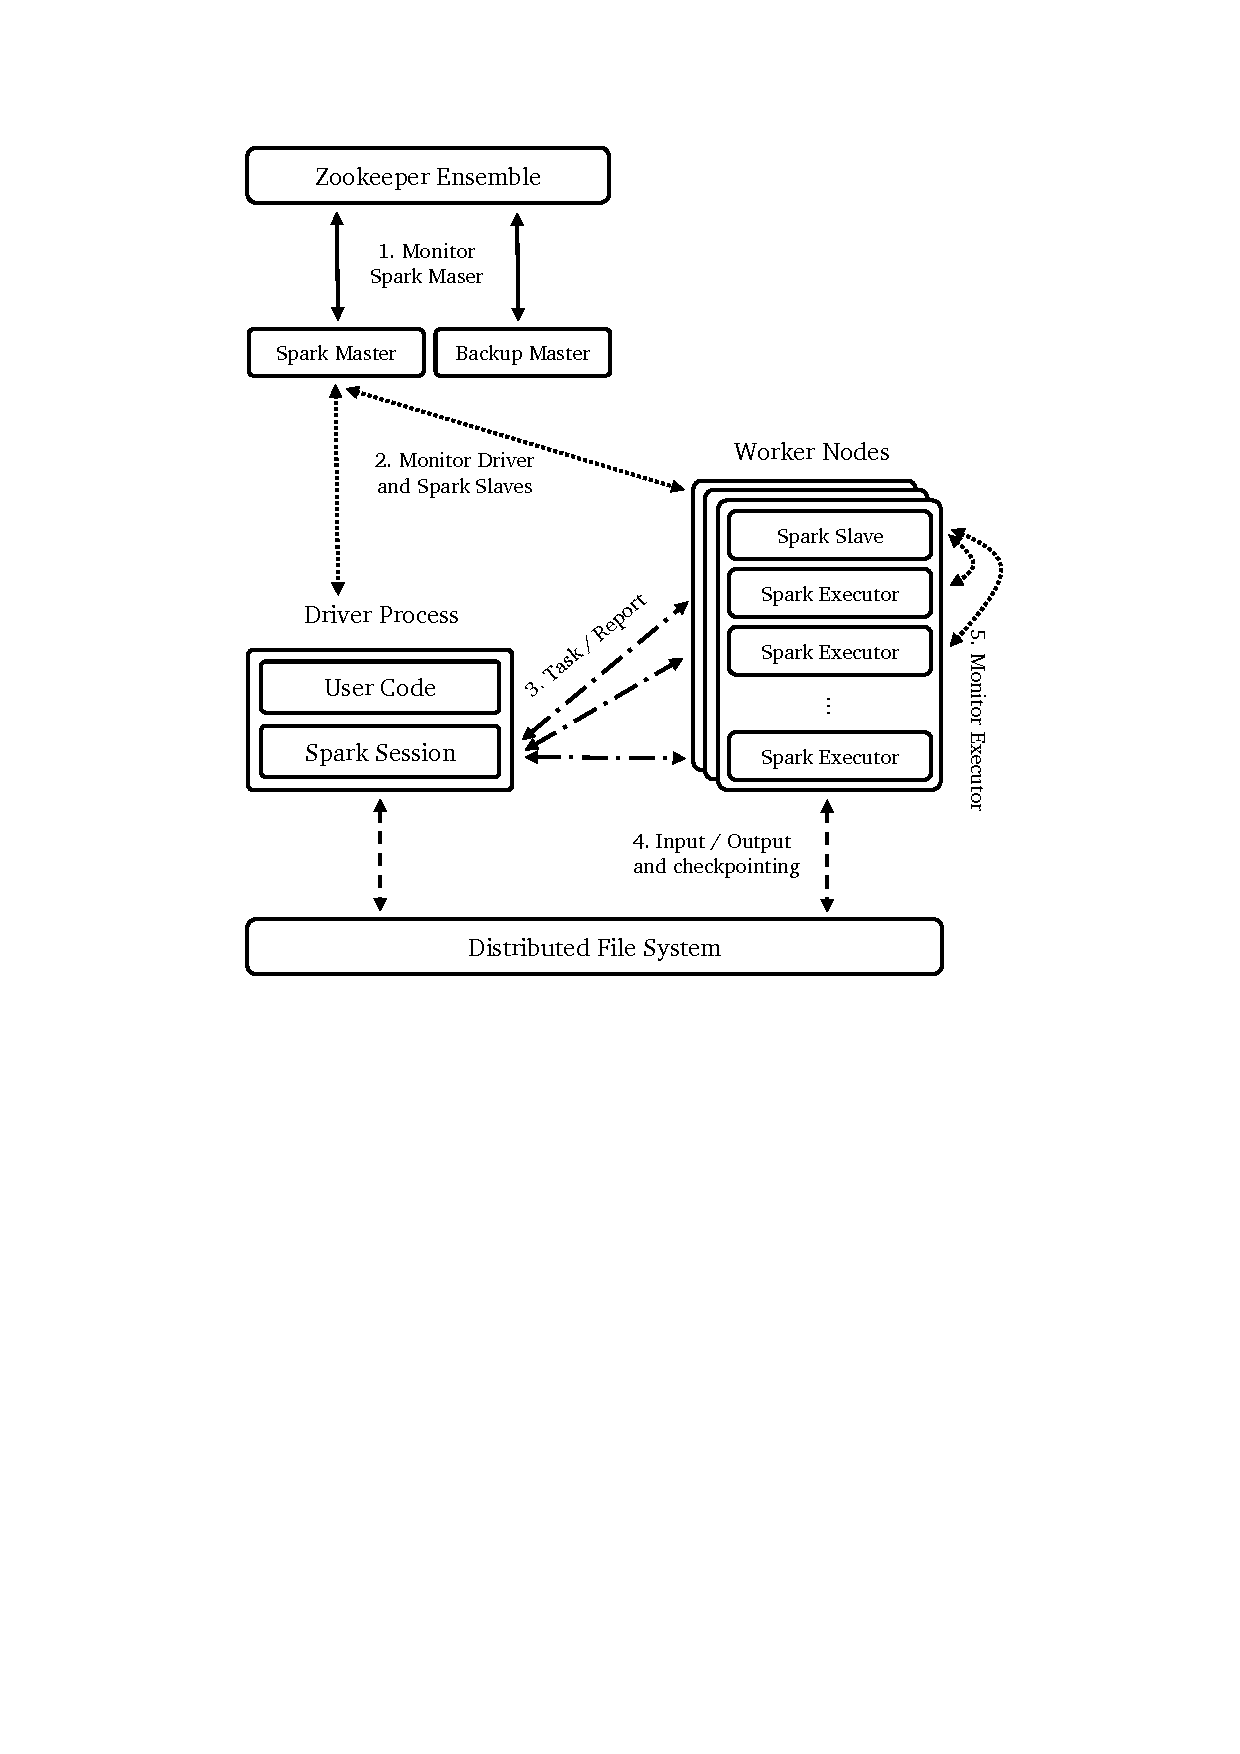
\includegraphics[clip,trim=4cm 13cm 4cm 2.2cm]{spark-full.pdf}
         \caption{Architecture of Spark Fault-Tolerance}
         \label{fig:spark-full}
     \end{figure}
\end{description}

\section{Resilient Distributed Datasets}
\label{sp:rdd}

\emph{Resilient Distributed Dataset} (RDD)~\cite{Zaharia:2012} is the basic building block of Spark's data processing pipeline. It is inspired by the same concepts behind \emph{shared memory} and enables \emph{iterative algorithms} and \emph{interactive analytics} to perform common operations directly on memory. RDDs are fault-tolerant and parallel data structures to let intermediate results of a Spark application to be stored in memory during multiple iterations. Existing distributed shared memory abstractions for cluster computing provide \emph{fine-grained} interface -- typically key/value -- to modify state. Unfortunately, with this approach the only way to provide fault-tolerance is the \emph{log shipping} approach that is already offered by distributed database systems.

Whereas, RDDs offer \emph{coarse-grained} interface based on \emph{immutable transformations}. Each transformation (\lstinline$map$, \lstinline$filter$, \lstinline$foreach$, \lstinline$groupByKey$, etc.) applies same application logic to all records that it contains. A dataset's \emph{lineage graph} is the \emph{chain}~-- \emph{sequence} -- of multiple transformations that produced the aforementioned dataset. With this approach only the transformation itself needs to be logged and shipped to other nodes to provide fault-tolerance. Since RDDs are already immutable, recomputing the lineage on other node is a trivial task. The RDD abstraction is useful in data intensive processing applications, since same operation is applied to many records. Table~\ref{tab:rdd-vs-dsm}\footnote{The table has been taken from~\textcite{Zaharia:2012}} summarizes the differences between RRDs and common distributed shared memory technologies.
\begin{table*}[h]
    \begin{tabular}{lll}
        \toprule
        \textbf{Dimension} & \textbf{RDD} & \textbf{Distributed Shared Memory}\\
        \midrule
        Reads & Per record or per input file & Per key/value \\
        Writes & Coarse grained & Per key/value \\
        Consistency & Easy (Immutable RDDs) & Application dependent \\
        Fault-Tolerance & Lineage recomputation & Application dependent \\
        Straggler Mitigation & Parallel backup tasks & Application dependent \\
        Operator Placement & Based on data locality & Application dependent \\
        Behavior if not enough memory is available & Controlled serialization to disk & OS managed swapping\\
        \bottomrule
    \end{tabular}
    \centering
    \caption{High-Level Comparison of RDDs and Distributed Shared Memory Systems}
    \label{tab:rdd-vs-dsm}
\end{table*}

An RDD is a \emph{read-only}, \emph{partitioned} collection of records~\cite{Zaharia:2012}. RDDs can only be created through deterministic transformations from either \emph{stable stoage} or \emph{other RRDs}.
\begin{itemize}
    \item \textbf{Stable storage}. In this case dataset is typically stored on a shared file system like HDFS and accessible from all nodes of the cluster.
    \item \textbf{Other RDDs}. In this case subsequent RDDs \emph{depend} on each other forming the lineage graph.
\end{itemize}

An RDD has enough information about how it was derived from other RDDs. This means it doesn't have to be materialized in every step of the pipeline. In other words, an RDD cannot reference another RDD that it cannot reconstruct after a failure. Additionally, users are able to control \emph{persistency} and \emph{partitioning} of RDDs.
\begin{itemize}
    \item \textbf{Persistency}. Users can define which RDDs will be reused in next steps of the pipeline. They choose a storage strategy -- in-memory or disk-based -- to persist RDDs.
    \item \textbf{Partitioning}. Some transformations like \lstinline$groupByKey$ or \lstinline$join$ partition the original RDD into multiple secondary partitions. RDDs allow application developers to perform partitioning -- hash, range or any custom partitioning strategy -- such that relevant records are \emph{co-partitioned} on same machine. This is particularly useful for \emph{operator placement} optimizations.
\end{itemize}

In order to simplify the concept of lineage graph, listing~\ref{l:sp:log-error}\footnotemark and figure~\ref{fig:spark-lineage-sample}\footnotemark[\value{footnote}] illustrate a simple log processing pipeline and its corresponding generated lineage graph.
\footnotetext{The figure and sample code has been partially taken from~\textcite{Zaharia:2012}}
\begin{lstlisting}[float=h, caption={Parsing Errors in Log Files From HDFS},label={l:sp:log-error},captionpos=b,morekeywords={val}]
val lines = spark.textFile("hdfs://...")
val errors = lines.filter(_.startsWith("ERROR"))
errors.persist()

// Case 1 -- Count total number of errors
val errorCount = errors.count()

// Case 2 -- MySQL error
val mysqlErrors = errors.filter(_.contains("MySQL"))
val mysqlErrorCount = mysqlErrors.count()

// Case 3 - Return forth field of MySQL logs that contain SLOW QUERY
val slowQueries = mysqlErrors.filter(_.contains("SLOW QUERY"))
                                                         .map(_.split(',')(3))
                                                         .collect()
\end{lstlisting}
\begin{figure}[p]
    \centering
    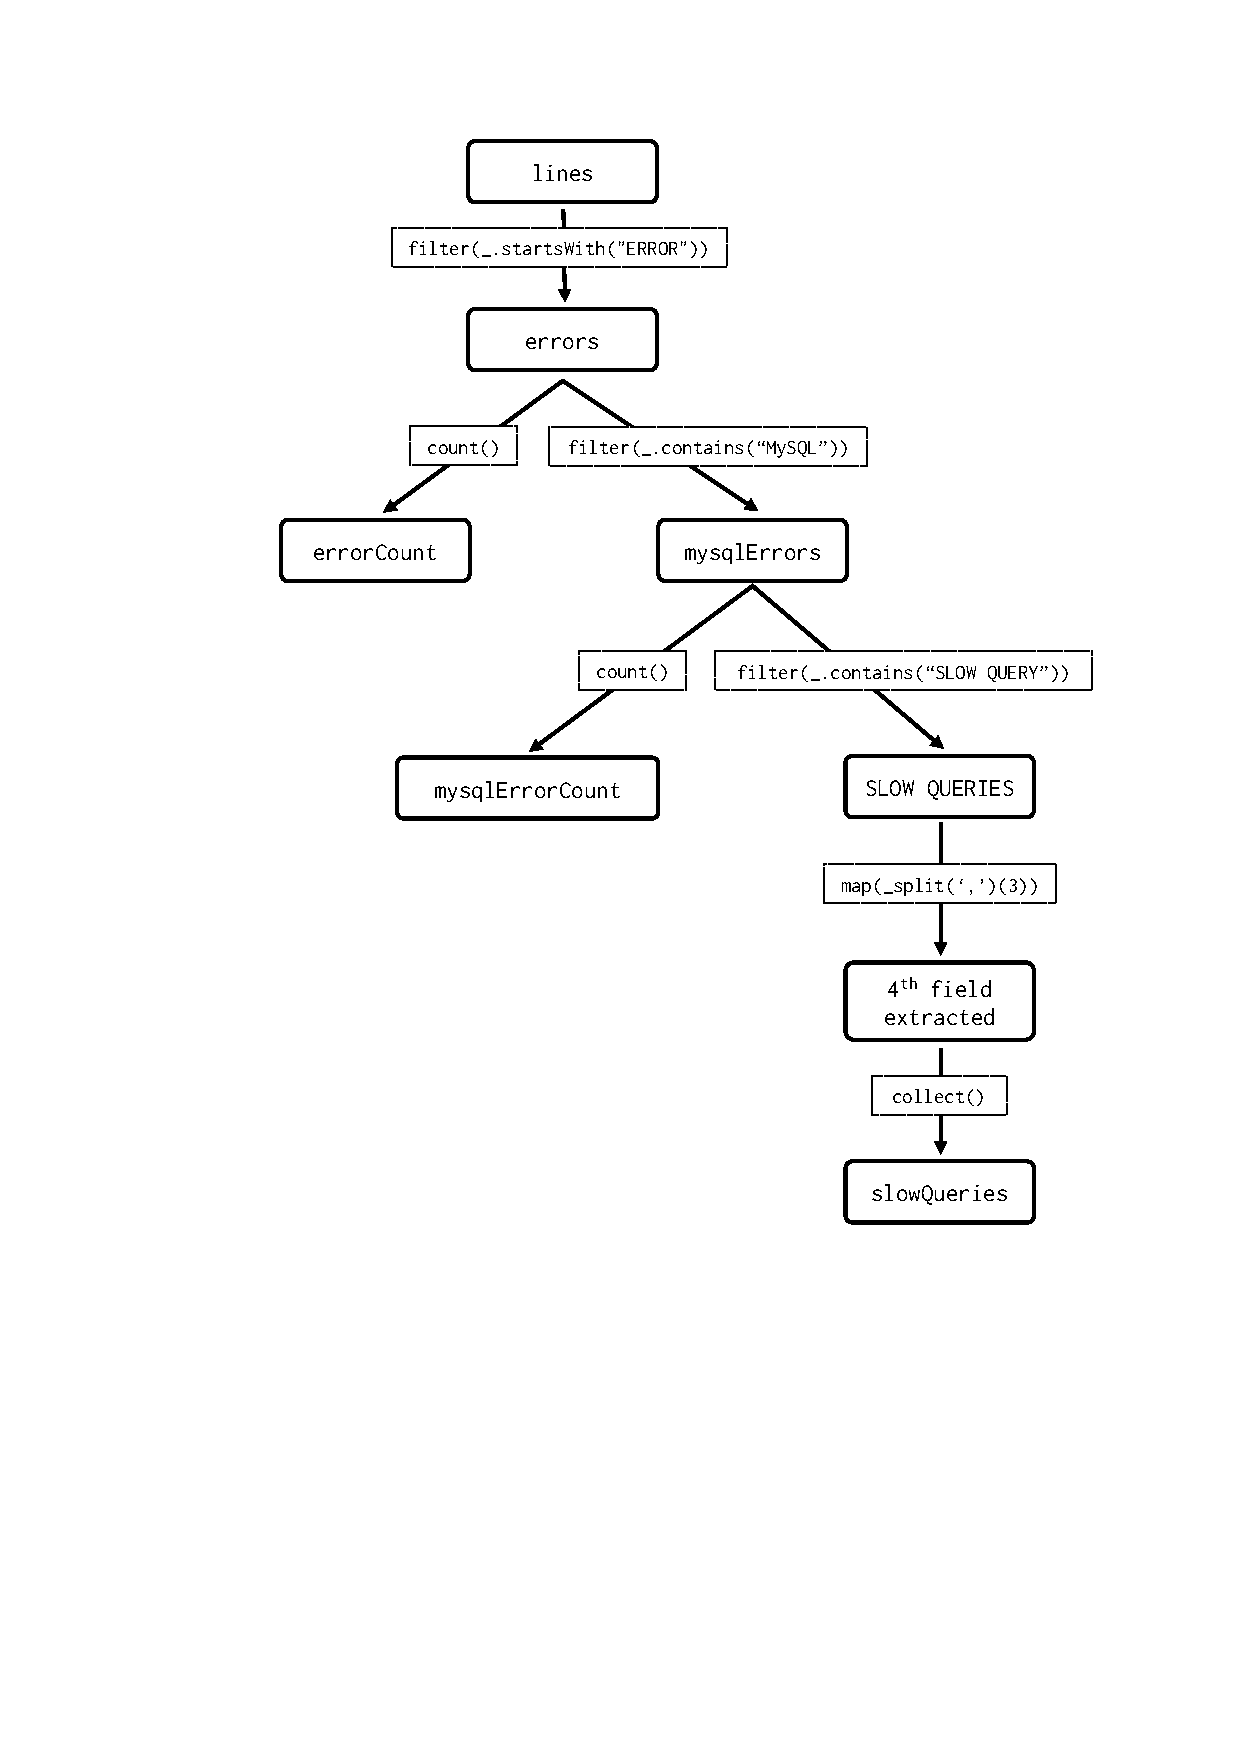
\includegraphics[clip,trim=4.5cm 8.9cm 2.2cm 2.2cm]{spark-lineage-sample.pdf}
    \caption{RDD Transformations and Corresponding Lineage Graph}
    \label{fig:spark-lineage-sample}
\end{figure}

\clearpage
\subsection{RDD Transformations and Dependencies}
\label{sp:depend}

As mentioned, RDDs are the result of \emph{lazy} transformations derived from one another. In other words, RDDs are not materialized unless it is really needed. However, not all transformations are lazy. There are three major types of transformations.
\begin{itemize}
    \item \textbf{Transformations without shuffling}. These are lazy transformations that doesn't cause any sort of shuffling among different nodes. That is, transformed records can still be further processed on the same node. For example, \lstinline$map$ and \lstinline$filter$ are classified in this group.
    \item \textbf{Transformations with shuffling}. These are also lazy transformations but they will trigger shuffling process between nodes. The behavior of the shuffling process is influenced by the implementation of \emph{partitioners}. As an example, \lstinline$groupByKey$, \lstinline$reduceByKey$ and \lstinline$join$ belong to this group.
    \item \textbf{Actions}. These transformations trigger RDD materialization process. That is, the actual computation of RDDs does not realize until this type of transformation is met in lineage graph. For example, \lstinline$count$, \lstinline$collect$ and \lstinline$save$ are classified in this group.
\end{itemize}

In a lineage graph, RDDs are derived from one another. This makes each RDD depend on one or several RDDs. There are two types of dependencies among RDDs.
\begin{itemize}
    \item \textbf{Narrow}. When one partition of the parent RDD is used by at most one partition of the child RDD, then the dependency is considered as narrow. For example \lstinline$map$, \lstinline$filter$, \lstinline$union$ and joins with \emph{co-partitioned} inputs create narrow dependencies. Narrow dependencies allow to process RDDs without triggering shuffling process -- a phenomenon known as \emph{pipelined execution}. Additionally, failure recovery is easier in case of narrow dependencies because only lost parent RDDs need to be recomputed. Figure~\ref{fig:sp:narrow-dep}\footnotemark depicts narrow dependencies.
    \item \textbf{Wide}. When one partition of the parent RDD is used by more than one partition of the child RDD, then the dependency is considered as wide. For example, \lstinline$groupByKey$ and joins with inputs \emph{not co-partitioned} create wide dependencies. Wide dependencies trigger the shuffling process. In contrast to narrow dependencies, recovering from node failures are less efficient since a failed node might cause loss of some partitions from all ancestors which requires full recomputation~\cite{Zaharia:2012}. Figure~\ref{fig:sp:wide-dep}\footnotemark[\value{footnote}] depicts wide dependencies.
    \begin{figure}[p]
        \centering
        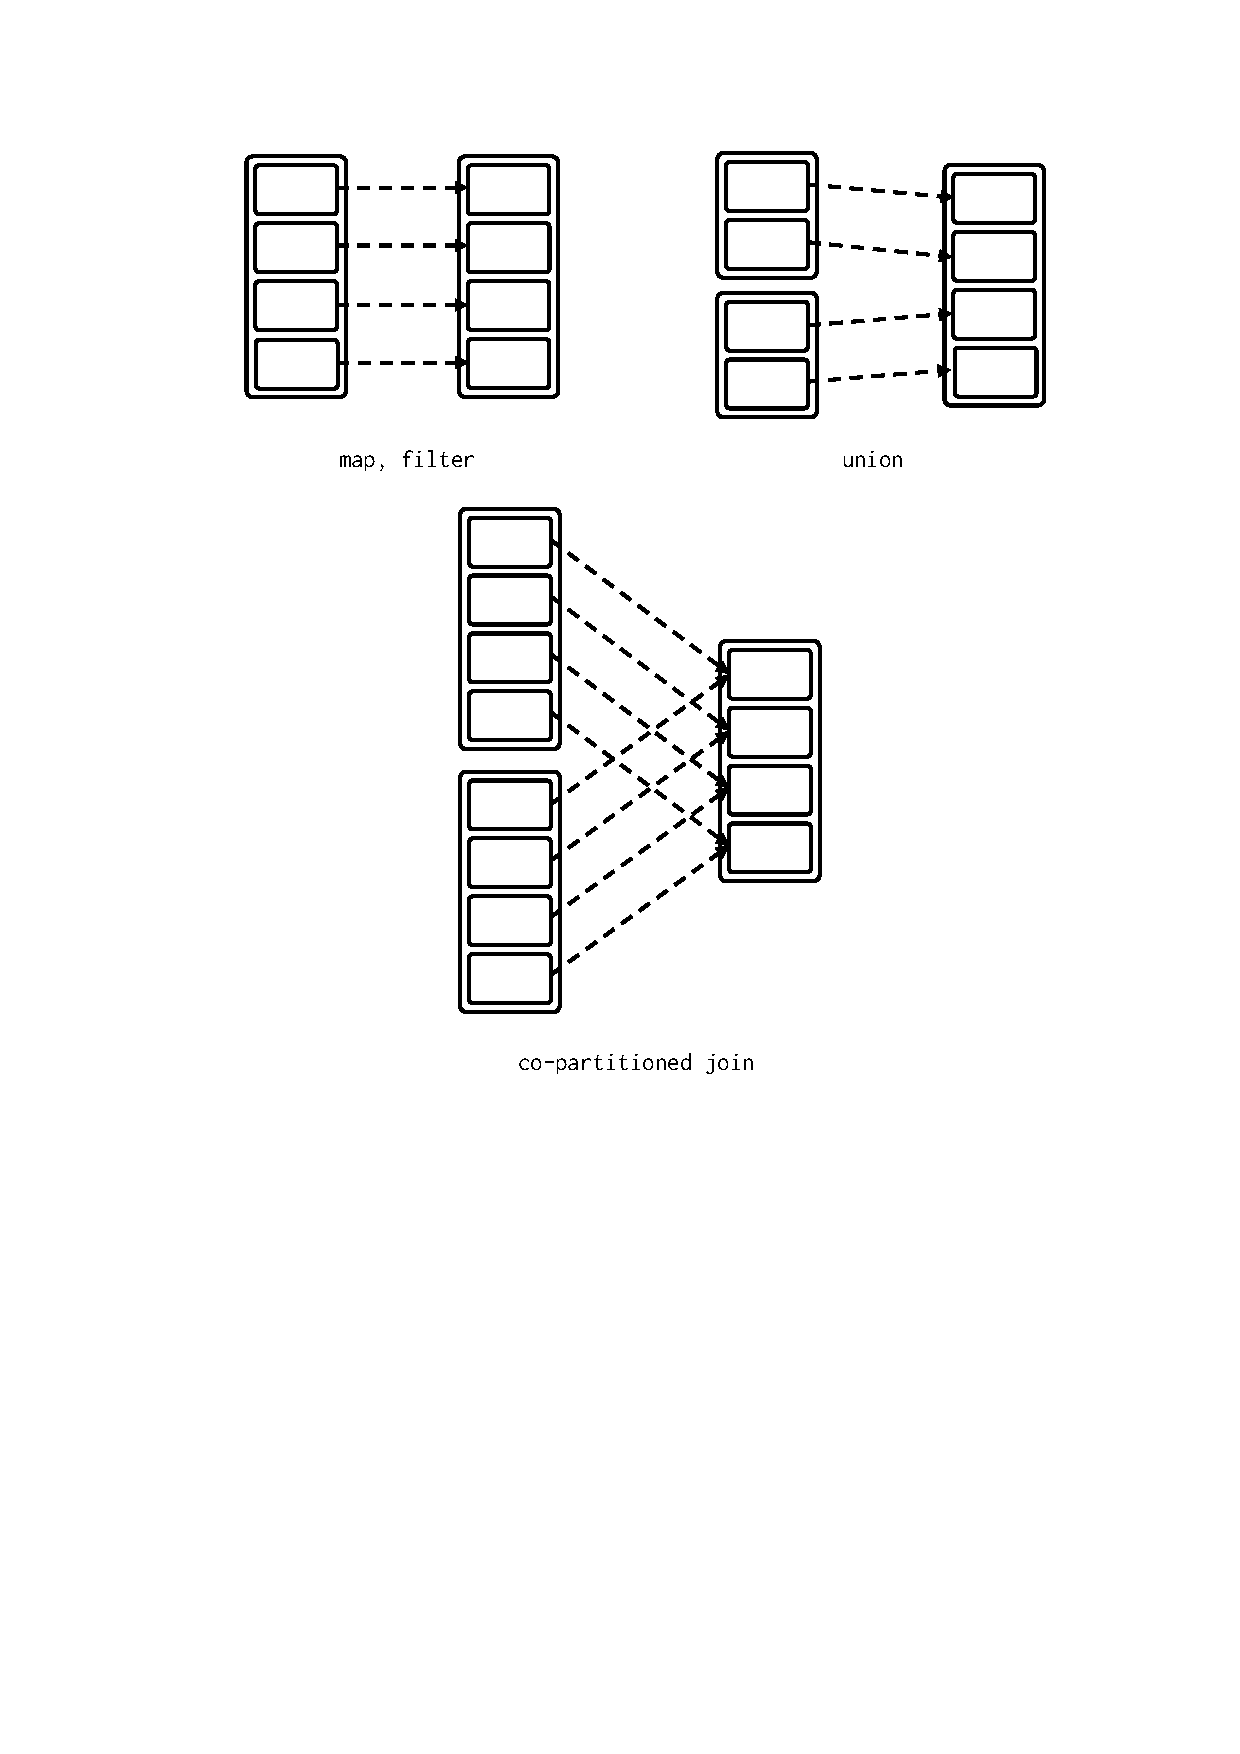
\includegraphics[clip,trim=4cm 11.5cm 3.1cm 2.5cm]{narrow-dep.pdf}
        \caption{RDD Narrow Dependencies}
        \label{fig:sp:narrow-dep}
        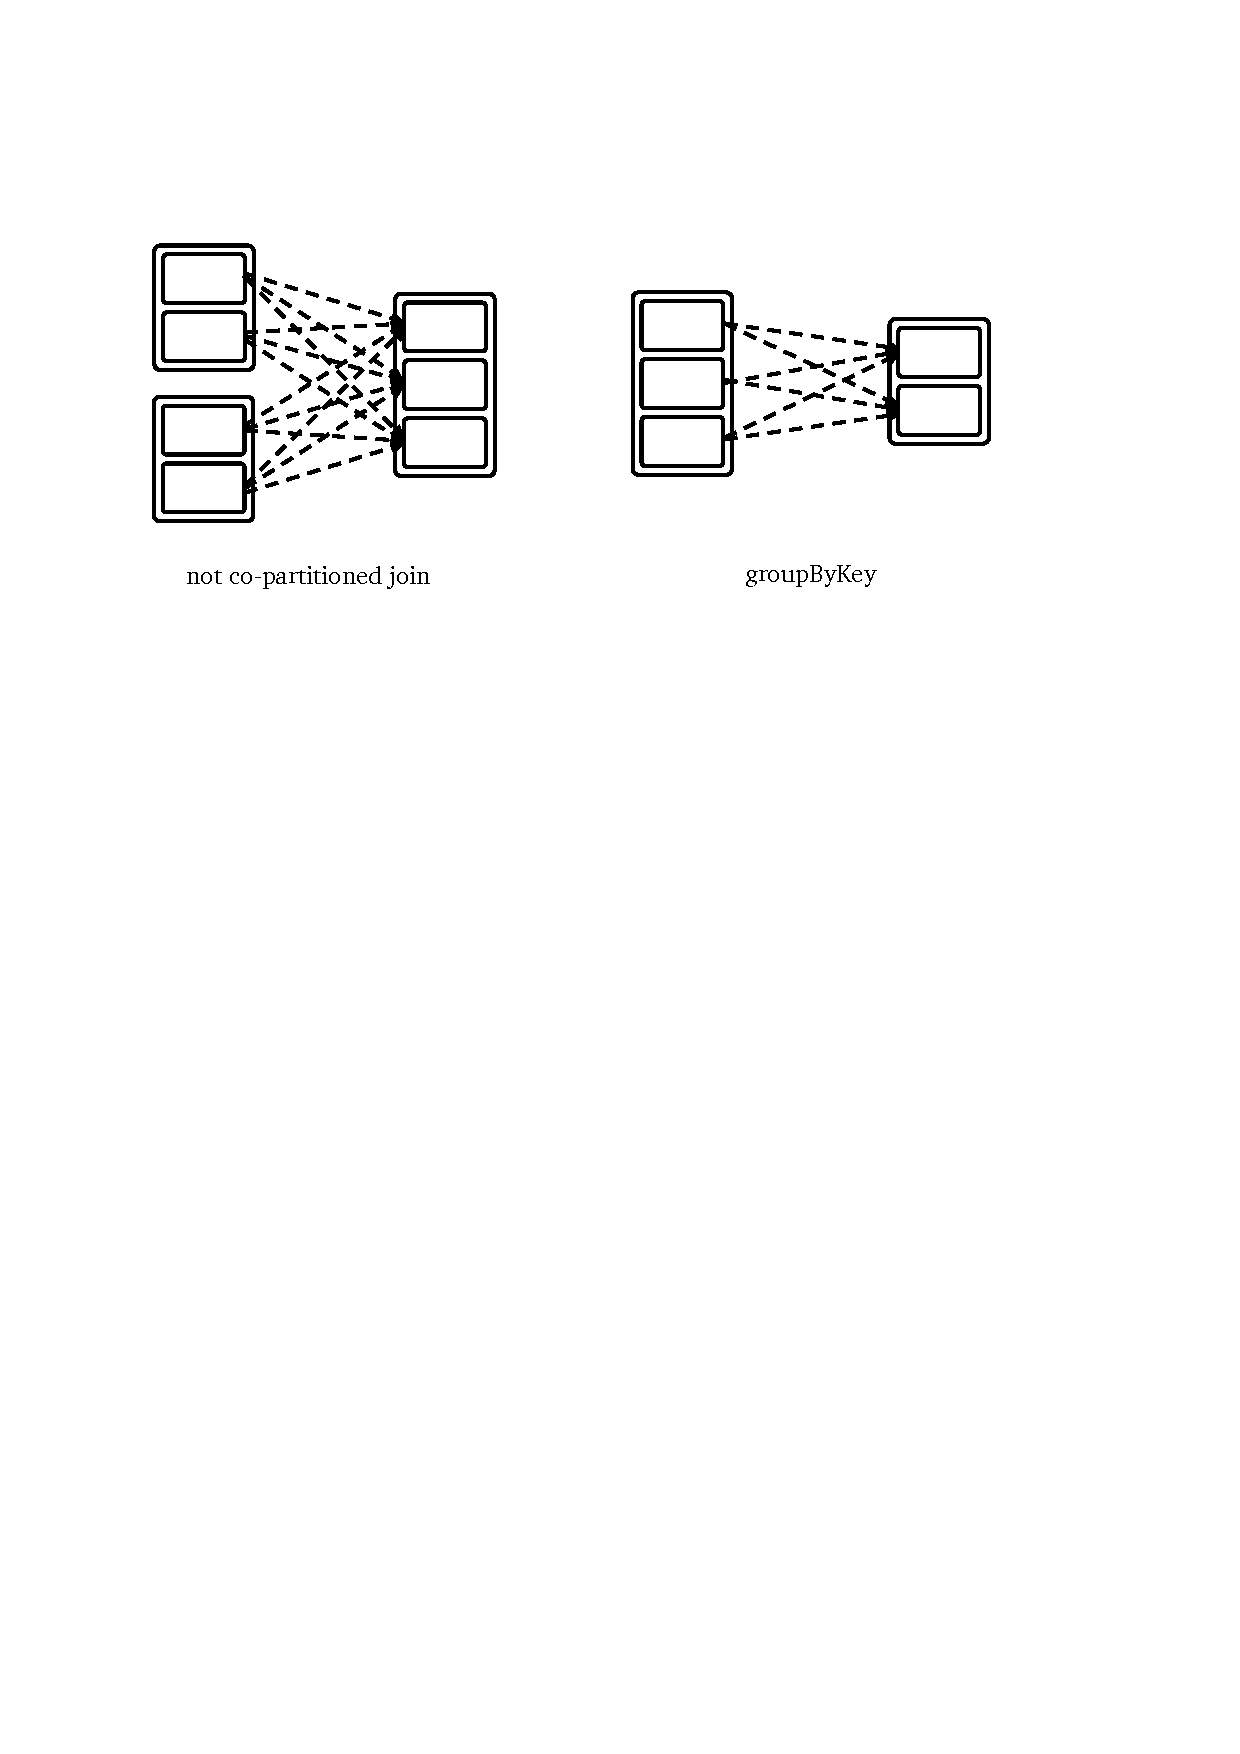
\includegraphics[clip,trim=2cm 19.5cm 3.5cm 4cm]{wide-dep.pdf}
        \caption{RDD Wide Dependencies}
        \label{fig:sp:wide-dep}
    \end{figure}
\end{itemize}
\footnotetext{The figure has been partially taken from~\textcite{Zaharia:2012}}

\subsection{Fault-Tolerance with Checkpointing}
\label{sp:fault}

The idea of the lineage graph and recomputable transformations significantly simplifies fault-recovery. However, in long chains recomputing failed RDDs can be a very time/process intensive operation. Hence, in some cases it is useful to checkpoint some RDDs to stable storage -- like shared file system. In general checkpointing is useful for applications with deep lineage graphs containing wide dependencies, since a node failure in parent RDDs leads to full recomputation in child RDDs. If the lineage graph is small or most dependencies are narrow, checkpointing tends to be less useful. 

In order to provide full control to application developers, Spark exposes checkpointing behavior though its API -- via \lstinline$REPLICATE$ flag in \lstinline$persist()$ function -- and leaves the decision up to developers. There are some scenarios where automatic checkpointing without intervention of developers may seem a feasible choice. Because job scheduler is completely aware of the size all RDDs and naturally it should be able to implement more effective checkpointing strategy compared to developers. However, this feature is not currently available in Spark.

With checkpointing in-place, providing fault-tolerance becomes a fairly straightforward process. Note that, RDDs are immutable set of records. This feature makes it easy to flush them in a background process, since there is no \emph{concurrency} and \emph{consistency} concerns involved. Noteworthy, there is an additional fault-tolerance mechanism known as \emph{WAL-based fault-tolerance} for streaming pipelines. This topic is further discussed in section~\ref{sp:dstream}.

\clearpage
\subsection{RDDs and Spark Job Stages}
\label{sp:stage}

Spark's Job scheduler is similar to Dryad~\cite{Isard:2007}. However, it takes RDD locations into account as well, since some partitions of RDDs are cached into memory or persisted to stable storage. When a job is submitted, Spark's job scheduler does the following.
\begin{itemize}
    \item \textbf{Calculating Lineage Graph}. In this step, Spark calculates the lineage graph of RDDs with corresponding transformations and dependencies.
    \item \textbf{Defining Stages}. In this step Spark defines the stages required to run the job. From developer's point of view a job is a sequence of RDDs. However, at runtime a job is modeled as \emph{Direct Acyclic Graph} (DAG) of stages. A \emph{stage} is basically the longest possible chain of RDD transformations with shuffling operations in the boundaries. Additionally, different partitions of RDDs in their corresponding stages will also be computed. 
    \item \textbf{Launching Tasks}. In this step, Spark launches \emph{tasks} which is going to be run by executors. Each task processes one or multiple partitions of RDDs. Depending on the location of RDDs, tasks will be launched on machines with data-locality awareness to reduce network transmission. In case a task fails, it can be run as long as parent stages are still available. If one or more parent stages become unavailable, missing partitions from parent stages shall be recomputed according to lineage graph.
\end{itemize}
Figure~\ref{fig:sp:logical} shows a sample job with logical operators and Figure~\ref{fig:sp:dag} depicts its corresponding DAG with two stages at runtime.
\begin{figure}[h!]
    \centering
    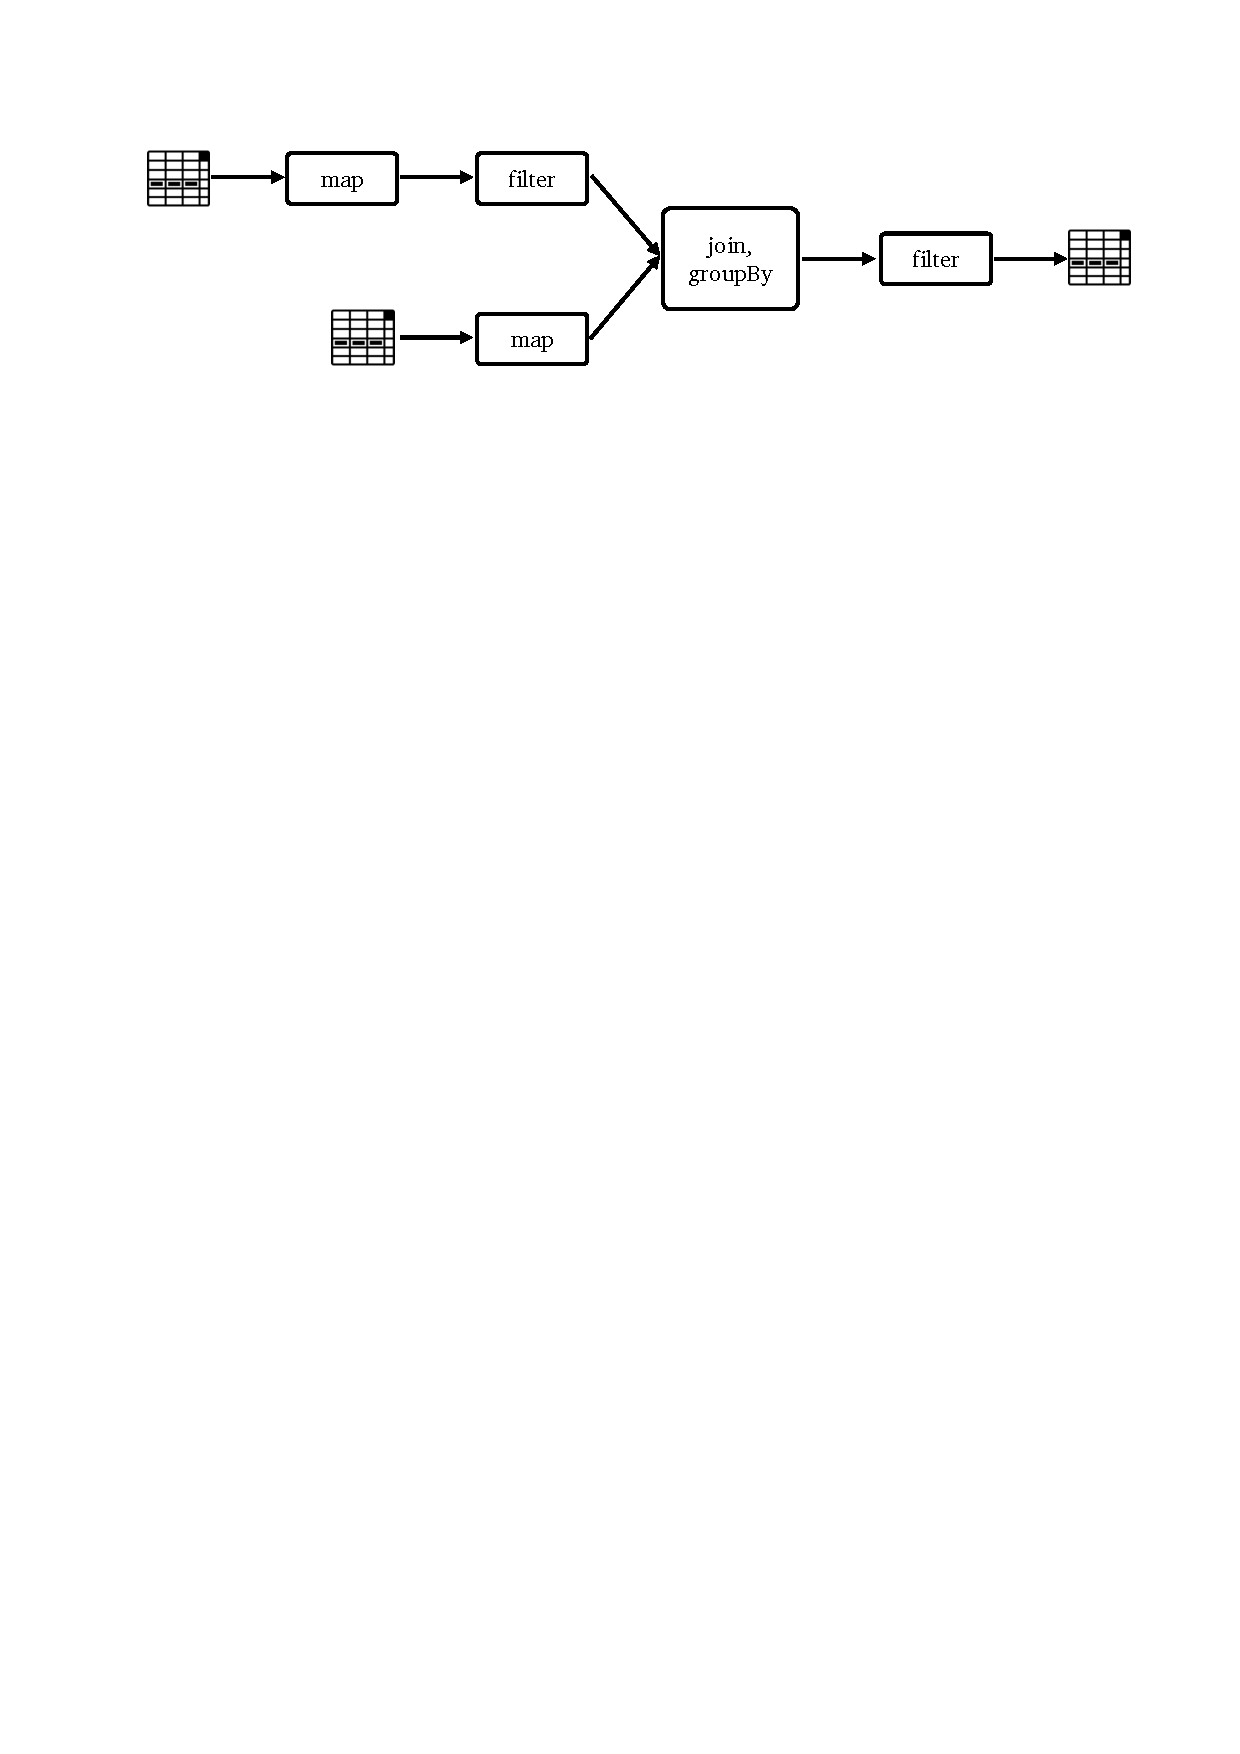
\includegraphics[clip,trim=2.3cm 23.5cm 1.7cm 2.5cm,scale=0.97]{stage-logical.pdf}
    \caption{Spark Job with Logical Operators}
    \label{fig:sp:logical}
    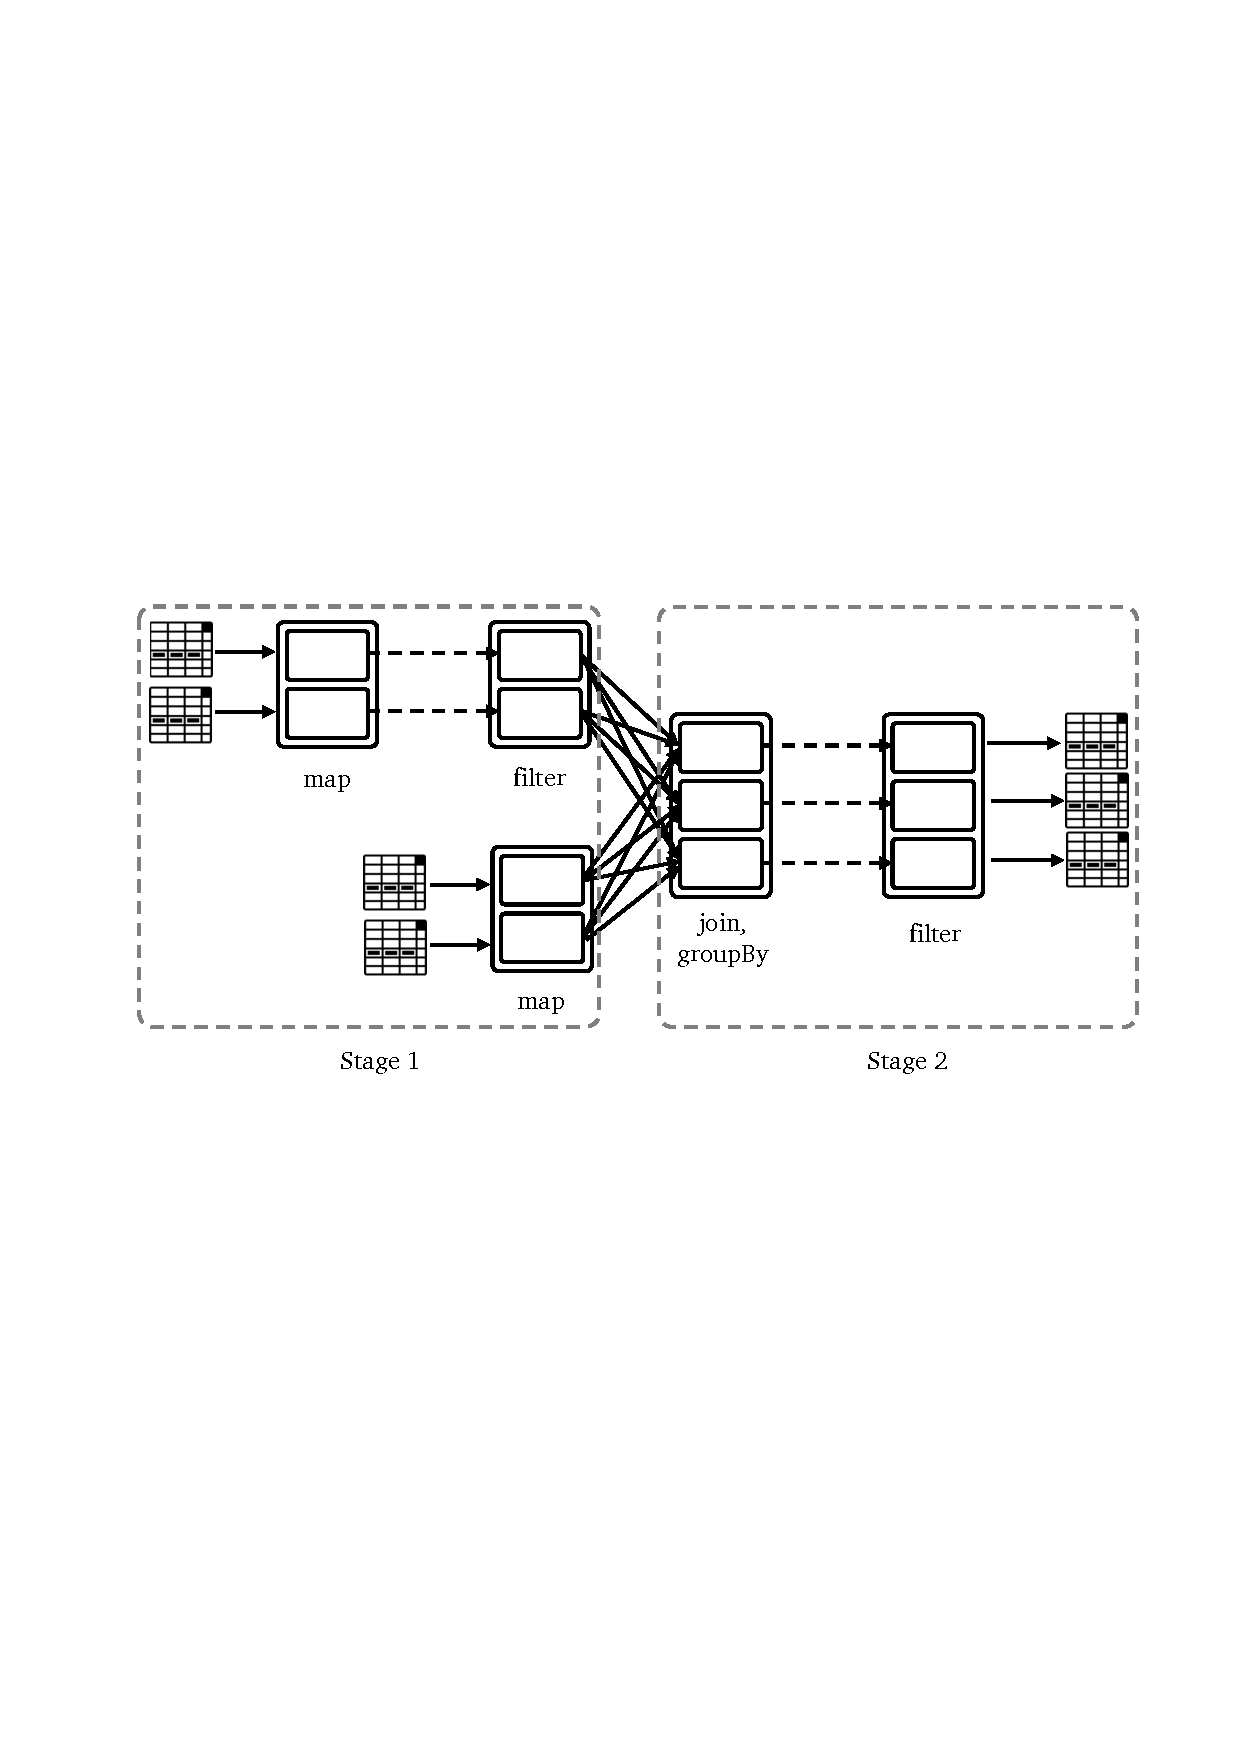
\includegraphics[clip,trim=2.3cm 11.4cm 1.7cm 10cm,scale=0.97]{stage-dag.pdf}
    \caption{Spark Job Stages at Runtime}
    \label{fig:sp:dag}
\end{figure}

\clearpage
\section{Discretized Streams}
\label{sp:dstream}

Many modern big data applications process data in real-time as they enter the processing pipeline. Online machine learning, fraud detection, spam detection, etc. are just few examples of applications that require near real time processing of data. In order to process incoming records in near real-time, new generation of data processing frameworks has been emerged which is known as \emph{stream processing systems}. Apache Storm~\cite{Storm} is an example of stream processing systems. Although these systems provide stream processing pipelines, but they also come with a couple of deficiencies. First, Section~\ref{sp:continues-model} explores the architecture of traditional stream processing systems and its problems. Then, Section~\ref{sp:dstream-model} describes the new stream processing model known as \emph{Discretized Streams} (D-Streams)~\cite{Zaharia:2013} that is built on top of RDDs in order to resolve the problems of traditional model.

\subsection{Continuous Operator Processing Model}
\label{sp:continues-model}

Although the concept of stream processing is nothing new and there has been many proposals and implementations like Apache Storm~\cite{Storm} and Apache Flink~\cite{flink}, but most of these systems are based on a processing model known as \emph{Continuous Operator Processing Model}. In this model streaming computations are divided into a set of \emph{long-lived stateful} operators that process messages in a loop:
\begin{enumerate}
    \item \label{sp:step-1}Get one or more messages from previous operators.
    \item Apply the computation -- business logic -- on newly received messages. Query the internal state if required.
    \item Update internal state if necessary.
    \item Produce any number of messages as the result of computation. These messages will be sent to next operators down the pipeline.
    \item Go back to Step~\ref{sp:step-1}
\end{enumerate}

While continuous processing model minimizes latency, the stateful architecture of operators and nondeterminism that comes from record interleaving on the network, makes it hard to provide fault tolerance efficiently. In particular, recovering from a \emph{failed} or slow node -- \emph{stragglers} -- is challenging. The are usually two standard approaches to overcome these issues.
\begin{description}[leftmargin=0pt]
    \item[Replication] In replication model which is borrowed from database systems, there are two copies of processing graphs. Produced messages are sent as duplicates to down stream operators. However, just replicating messages is not sufficient. A \emph{consensus protocol} should exist in-place to ensure that both operator replicas see incoming messages in the same order that is sent by upstream operators. Even though replication is a costly operation but it recovers from failures very fast, since both replicas are processing message online in synchronized steps.
    \item[Upstream Backup] The basic idea behind this model~\cite{Hwang:2005} is to checkpoint the internal state every once in a while to a stable shared storage. In case an operator -- or node -- fails, a backup operator takes over and reloads the last successfully written checkpoint. Then backup operator rebuilds the state by replying new messages and reproducing lost messages as necessary. Although this model is more efficient in terms of replication costs, but suffers from high fail-over time. Backup node should replay newly published messages from the last checkpoint and apply them to the internal state. Depending on checkpointing interval, this might be a time consuming operation.
\end{description}
Besides the fault-tolerance costs of this model, dealing with straggler nodes are even more challenging. Replication model provides no solution at all, since two replicas are processing messages synchronously. The only way to resolve this issue in Upstream Backup model is to fail -- kill -- the slow operator and let the backup operator takes over the responsibility which will undergo slow recovery process. Figure~\ref{fig:sp:cont-op} depicts these two approaches with additional synchronization and replication messages involved.
\begin{figure}[ht]
    \centering
    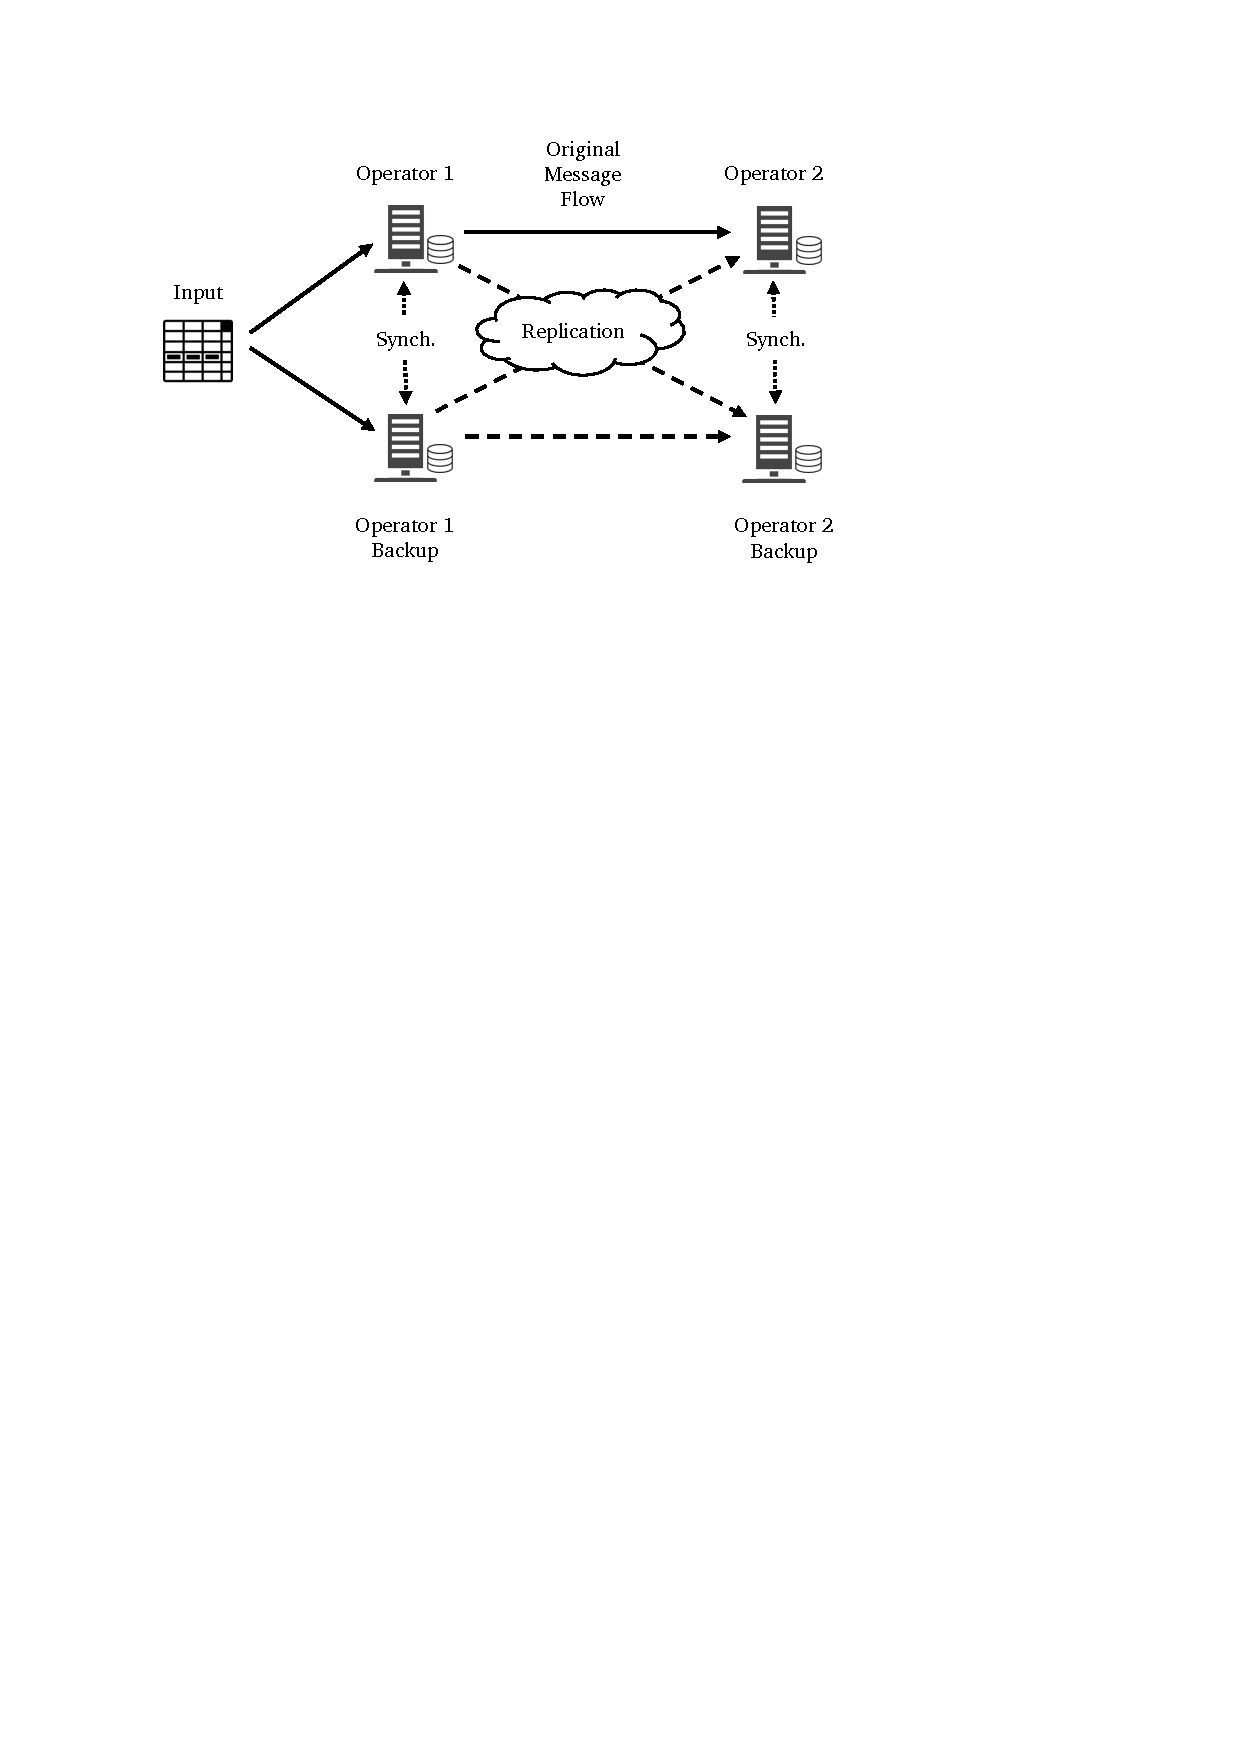
\includegraphics[clip,trim=2.5cm 20cm 6.7cm 2.2cm]{cont-op.pdf}
    \caption{Continuous Operator Processing Model}
    \label{fig:sp:cont-op}
\end{figure}

\subsection{D-Stream Processing Model}
\label{sp:dstream-model}

\emph{Discretized Streams} (D-Streams)~\cite{Zaharia:2013} is a novel technique to overcome the issues the Continuous Operator Processing Model. The basic idea behind D-Streams is to separate the computation from its state and keep the state as RDDs. This separation provides the following benefits.
\begin{itemize}
    \item Computation of messages becomes a set of \emph{stateless} and \emph{deterministic} tasks operating on RDDs.
    \item RDDs already provide resiliency through in-memory replication and lineage recomputation. There is no need for further mechanisms to provide fault-tolerance.
    \item Unified processing model for batch and stream processing.
\end{itemize}

As a consequence of storing operator intermediate state as RDDs, a streaming computation can be modeled as series of \emph{deterministic batch computations} on small intervals -- known as micro-batch. Messages received in each batch interval is stored reliably across the cluster to form an input dataset for that interval. Once the time interval completes, this dataset is processed just like traditional batch processing using \lstinline$map$, \lstinline$filter$, \lstinline$groupByKey$, etc. Formally, a D-Stream is a sequence of \emph{immutable}, \emph{partitioned} datasets (RDDs) that can be acted on by deterministic transformations~\cite{Zaharia:2013}. These  transformations produce new D-Streams, and may create intermediate state represented as RDDs. Figure~\ref{fig:sp:dstream-high} shows high-level D-Stream computation model.
\begin{figure}[hb]
    \centering
    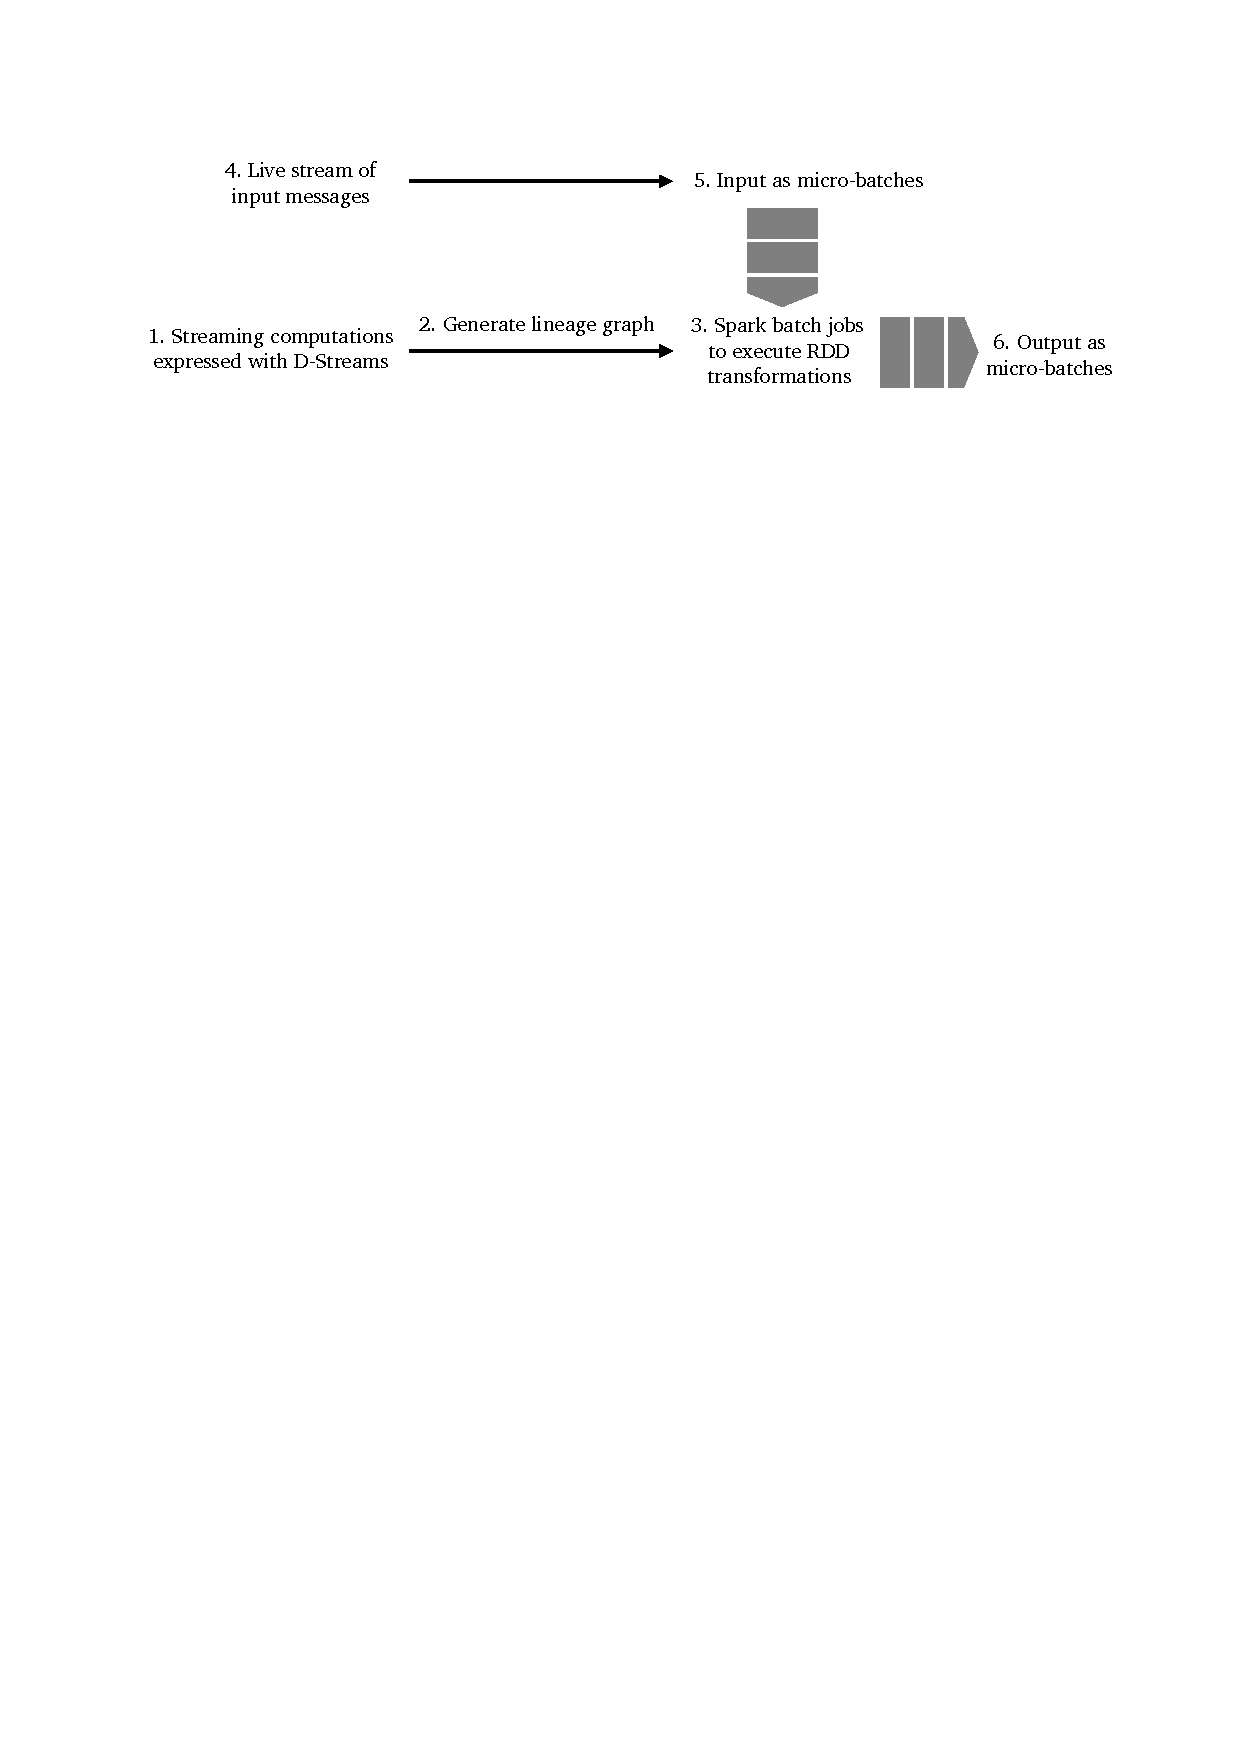
\includegraphics[clip,trim=2.1cm 23cm 2cm 2.6cm]{dstream-high.pdf}
    \caption{D-Stream High Level Processing Model}
    \label{fig:sp:dstream-high}
\end{figure}

In order to clarify D-Stream API, listing~\ref{l:sp:dstream-api}\footnotemark shows a simple streaming word count example. It creates a \lstinline$pageViews$ D-Stream by
reading event stream over TCP, and groups them into 1-second batch intervals. Then, it transforms the event stream to a new D-Stream of \lstinline$(URL,1)$ pairs called
\lstinline$ones$. Finally, it performs a running count with a \emph{stateful} \lstinline$runningReduce$ operator. Figure~\ref{fig:sp:dstream-api}\footnotemark[\value{footnote}] depicts the corresponding lineage graph and how the streams are divided into batch intervals. Note that smaller rectangles illustrates RDD partitions.
\begin{lstlisting}[float=h, caption={Streaming Word Count using D-Stream API},label={l:sp:dstream-api},captionpos=b,morekeywords={val}]
val pageViews = readStream("tcp://...", "1s")
val ones           = pageViews.map(event => (event.url, 1))
val counts       = ones.runningReduce((a, b) => a + b)
\end{lstlisting}
\begin{figure}[h]
    \centering
    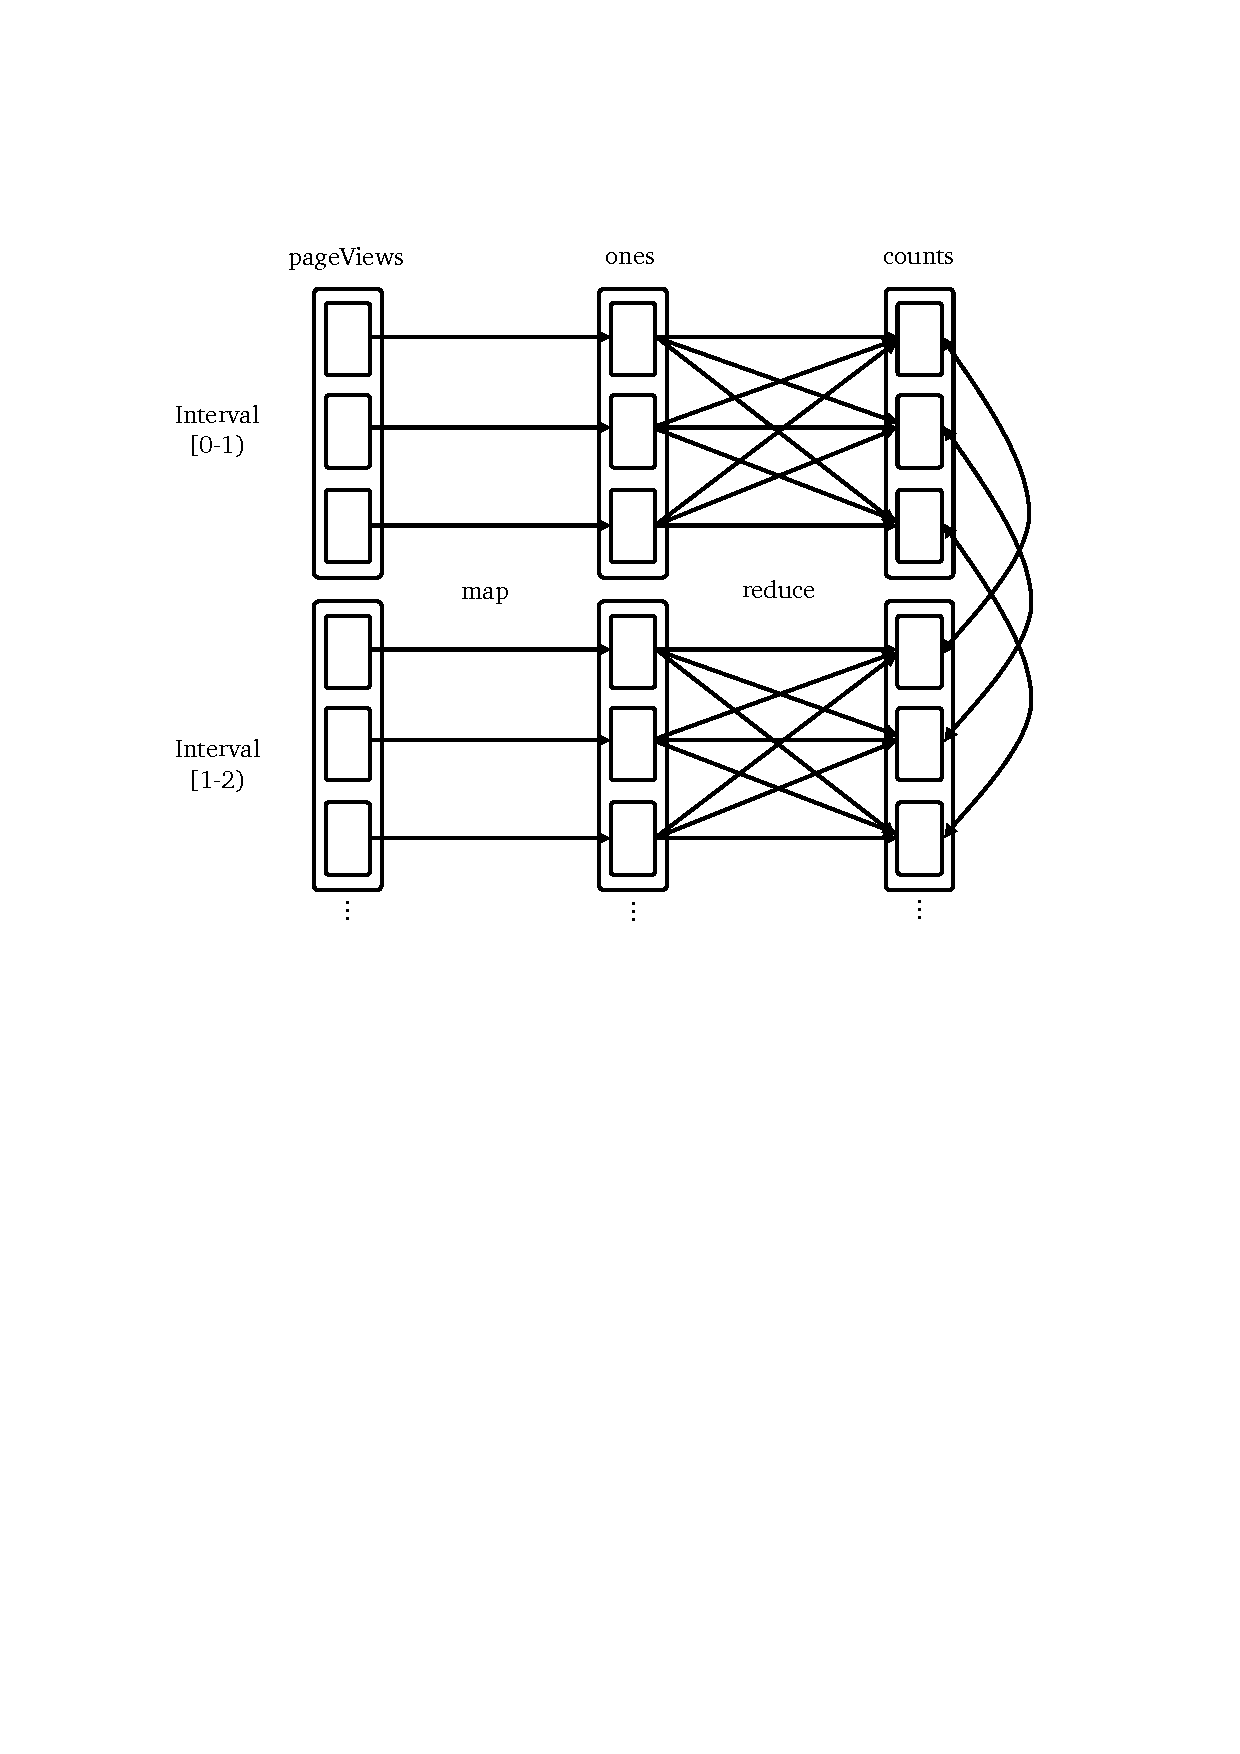
\includegraphics[clip,trim=2.5cm 11cm 3cm 4cm]{dstream-example.pdf}
    \caption{Streaming Word Count Using D-Stream API}
    \label{fig:sp:dstream-api}
\end{figure}
\footnotetext{The code and figure has been partially taken from~\textcite{Zaharia:2013}}

\clearpage
\subsection{Fault-Tolerant Message Consumption}
Since RDDs provide the basic building block of Spark Streaming, achieving fault-tolerance in streaming applications is a straightforward process. In case of any node failure, failed RDD partitions can be reproduced easily by evaluating lineage graph and determining which transformations need to be recomputed. Furthermore, for stateful transformations, Spark already provides checkpointing. However, there is one case that needs more attention.

Naturally, in streaming applications, live stream of records are coming from some data sources. For example, in log processing application it may originate from web servers or in live monitoring applications it comes from sensors. If one of the RDD transformations crashes during message consumption, two questions arise:
\begin{itemize}
    \item Are the messages that were consumed before crashing, be redelivered after relaunching failed transformations?
    \item In case lost messages are redelivered, will they be delivered with the same order as consumed before crashing?
\end{itemize}
The answer to these two questions leads us to \emph{three} types of data sources.
\begin{description}[leftmargin=0pt]
    \item[Reliable Ordered] With this type of data sources, the data source provides ordering and reliable message consumption capabilities. Messages will be kept in data source until its reliably confirmed -- ACKed -- by consumer. In case of consumer crash, messages will be delivered with the same order as before. Many of publish-subscribe message brokers such as Apache Kafka~\cite{kafka} provide this feature.
    \item[Reliable Unordered] With this type of data sources, the data source provides reliable message store but redelivery is not guaranteed to be in the same order as before consumer crash. For cases where ordered message consumption is crucial for business logic of the application, Spark Streaming provides \emph{WAL-based} consumers. With WAL-based consumers, each consumer appends the received message to a log file before starting to consume the message. These log files are stored in a distributed file system like HDFS. In case of consumer failure, another consumer re-opens the log file and re-processes the messages with same order as before.
    \item[Unreliable] This type of data source does not provide any form of reliability, ordering and fault-tolerance. Hence, WAL-based message consumption shall be enabled by application developer.
\end{description}

\section{Conclusion}
\label{sp:conc}

In this chapter different aspects and features of Spark has been explored. Built on top of unique features of Resilient Distributed Datasets (RDDs), Spark offers a unified approach for batch and stream processing. As explained during the chapter, deficiencies and problems of traditional systems have been addressed to some extent by Spark.
\chapter{Design and Implementation Detail}
\label{design}

\section{Introduction}
\label{des:intro}

In this chapter design and project structure of implemented techniques will be introduced and discussed. Two techniques have been selected to be implemented. This chapter is organized as follows. Section~\ref{des:choose} explains selected techniques and the reasoning behind it. In this section, selected techniques are explained at theoretical level. Section~\ref{des:proj} describes the structure of the implementation for Spark Streaming in detail. Section~\ref{des:conf} describes the configuration parameters required to launch the implementation. Finally, Section~\ref{des:conc} concludes this chapter.

\section{Choosing Auto-Scaling Techniques}
\label{des:choose}

As discussed in Section~\ref{ias:alg-fam}, Auto-Scalers can be categorized into 5 groups.
\begin{description}[leftmargin=0pt]
    \item[Threshold-Based] In this approach, one or multiple threshold values are defined~\cite{Hasan2012IntegratedAA} which specifies the behavior of the Auto-Scaler when the system load goes beyond these thresholds. However, manually defining thresholds is a tricky process~\cite{Dutreilh2010}. Spark's default dynamic resource manager~\cite{spark} and Online Parameter Optimization~\cite{Heinze:2015} are partially based on this approach and they will be evaluated in Section~\ref{eval}.
    \item[Time-Series Analysis] In this approach, a history window of workload -- depending on prediction accuracy -- is considered to predict future workload. However, in case the workload is changing in an unpredictable way -- which is not an unusual phenomena in streaming applications -- then this approach becomes less useful. As confirmed by DEBS grand challenges~\cite{debs2014}~\cite{debs2015}~\cite{debs2016}, the general assumption for streaming applications is that the workload is unpredictable. Due to this limited applicability, no time-series technique is implemented.
    \item[Queuing Theory] In this approach, the system is modeled as a queue network. Since queuing parameters -- message inter-arrival and service rates --  are static, they have to be re-calculated in a timely manner. One of the novel implementations is done by~\textcite{Lohrmann:2015}. However, authors made two unconvincing assumptions. First, worker nodes shall be homogeneous in terms of processing power and network bandwidth. Second, there should be an effective partitioning strategy in place in order to load balance outgoing messages between stages. In reality both assumptions rarely occur. Large scale stream processing clusters are built incrementally. Depending on workload, data skew does exist and imperfect hash functions are widely used by software developers. Furthermore, as confirmed by~\textcite{Rajarshi:2005}, queuing models are very complicated to build and less adaptive to changing environments. As a consequence, no queuing theory technique is implemented.
    \item[Reinforcement Learning] Reinforcement Learning has shown its capabilities to adapt ever changing environments. However, some of the proposed solutions are conflicting with the requirement of this thesis as discussed in Section~\ref{prob-def}. The following summarizes the reasoning why each proposal is accepted or rejected by this thesis.
    \begin{itemize}
        \item \textcite{Herbst:2017} proposed a solution based \emph{Bayesian Networks}. There are two major problems with this proposal. First, it needs sampling and offline training which is inapplicable for changing streaming workloads. Second, in case the model is complex, the training phase is long and computationally infeasible for streaming workloads. As mentioned, both issues are conflicting with thesis requirements.
        \item \textcite{Tesauro2006} proposes a hybrid approach to resolve performance issues of online training which consists of two components. First an online component based on queuing theory. Second, Reinforcement Learning component that is trained offline. This proposal models each node as a queue. However, the only way to apply this technique is to modify \lstinline$spark-core$ package. Thus, this solution is not implemented.
        \item \textcite{Rao:2009:VRL} proposed a solution to manage virtual machine resources. However, it is also based on offline training and sampling which is obtained from a separate supervised training phase. Thus, it's not applicable for dynamic streaming workloads. 
        \item \textcite{Enda:2012} proposed a parallel architecture to Reinforcement Learning without any global controller involved. Nodes (RL agents) have two tables. Local table is trained by each node separately. Global table contains values learned by other nodes. When an agent learns anything new, it broadcasts it to other nodes. From theoretical point of view, this solution might seem feasible, since parallel learning speeds up initialization process. However, Spark has a single global controller. Applying this technique to Spark requires heavy modification to \lstinline$spark-core$ package. 
        \item \textcite{Heinze:2014} implemented Reinforcement Learning in the context of FUGU~\cite{Grandl:2014:MPC}. Each node, maintains its own Q-Table and imposes local policy without coordinating with other nodes. Although this architecture is not applicable for Spark, but its core idea -- \emph{Temporal Difference}~\cite{rlIntro} algorithm-- is applicable. Thus, this thesis implemented this proposal by adopting it to Spark architecture. Refer to Section~\ref{des:temp} for theoretical background and Section~\ref{des:proj} for implementation detail.
        \item \textcite{CARDELLINI2018171} proposed a two level hierarchical architecture for resource management in Apache Storm~\cite{Storm}. Local controller applies local policy on each node and coordinates with the global controller for confirmation of its actions. Although, this architecture seems to be a promising approach, however it has been implemented by modifying Storm's internal components. As mentioned above, this is in conflict with thesis's requirements.
        \item \textcite{dutreilh:hal-01122123} proposed a model-based Reinforcement Learning approach for resource management which is based on a global controller. In order to overcome the slow convergence of model-free learning, authors proposed to estimate environment dynamics based on collected samples at runtime. Then it switches to \emph{Value Iteration}~\cite{rlIntro} algorithm instead of \emph{Temporal Difference}. This approach has also been partially adopted by this thesis. Refer to Section~\ref{des:val} for theoretical background and Section~\ref{des:proj} for implementation detail.
    \end{itemize}
    \item[Control Theory] Techniques based on Control Theory are also promising for elastic data streaming. Because it monitors input and output of the application, it can respond to workload changes very fast and adapt the system if necessary. Thus it is perfectly capable of handling dynamic environments. The comparison between Reinforcement Learning and Control Theory techniques is left for future work.
\end{description}
As mentioned, two techniques -- \emph{Temporal Difference} and \emph{Value Iteration} -- will be implemented in this thesis. In next two sections, theoretical foundation of these algorithms will be laid out. Noteworthy to mention, these sections are heavily inspired by~\textcite{rlIntro}. Furthermore, Section~\ref{related} discusses more techniques and the reasoning why they have been rejected by this thesis.
\clearpage
\subsection{Temporal Difference}
\label{des:temp}
Section~\ref{ias:alg-rl} explains the basics of Reinforcement Learning. Temporal Difference (TD) learning is one of the foundational algorithms of Reinforcement Learning. It can learn from applying experience without having prior knowledge about environment's dynamics. This property is potentially useful for data stream processing systems in which the incoming workload is changing without any particular pattern.

Before starting to dig into details, some formal notions shall to be explained. An \emph{episode} is series of experiences that is taken by the agent. At each time step~$t$, the agent moves from one \emph{state}~$S_t$ to another state~$S_{t+1}$. A \emph{policy} $\pi$ defines the action~$A_t$ that should be taken by the agent at each state. Followed by each action, the agent receives a \emph{reward}~$R_{t+1}$ from the environment. Note that, the agent will receive reward for its corresponding action at next state~$S_{t+1}$. Thus, an episode can be viewed as Equation~\ref{des:eq:episode}.
\begin{equation}
\dots\,S_t,\,A_t,\,R_{t+1},\,S_{t+1},\,A_{t+1},\,R_{t+2},\,S_{t+2},\,A_{t+2},\,R_{t+3}\,\dots
\label{des:eq:episode}
\end{equation}

An episode does not necessarily have a \emph{terminal} state. In some environments -- like data stream processing -- an episode is a never ending sequence of experiences. Prior to taking an action, the agent has an estimate of \emph{expected reward}~$V$ which specifies future reward if it follows the same actions returned by policy~$\pi$ from that specific state. Thus, it is referred as $V_\pi$ which translates to expected future reward under policy~$\pi$. During the episode, the agent tries to \emph{maximize} the reward that it received from the environment. Any policy that leads to maximum possible reward is called the \emph{optimal} policy~$\pi^*$ and its corresponding estimate of future reward is referred to as~$V^{*}_{\pi}$.

Unlike Monte Carlo~\cite{rlIntro} methods that requires agent to wait until the end of episode, TD approaches only need to wait until the end of next time step to get a feedback from environment. Then, the agent updates corresponding estimate of previous state. Thus, the most simple TD approach can be formulated as Equation~\ref{des:eq:std}. Equation~\ref{des:eq:std} contains two important parameters of TD.
\begin{equation}
V(S_t) \longleftarrow (1-\alpha)V(S_t) + \alpha\big[R_{t+1} + \gamma\,V(S_{t+1})\big]
\label{des:eq:std}
\end{equation}
\begin{itemize}
	\item $\bm{\alpha}$ denotes \emph{Learning Factor}. It specifies, how much the agent shall learn from new experiences. A higher $\alpha$ means learning with a faster pace. It also leads to forgetting history faster. On the other hand, a lower $\alpha$ leads to slower learning process which means the agent trusts its experience history more -- it gives more weight to history rather than new experiences. $\alpha$ is defined as a number between (0,1].
	\item $\bm{\gamma}$ denotes \emph{Reward Factor} or \emph{Discount Factor}. It specifies, whether the agent shall optimize for \emph{future} or \emph{immediate} reward. A higher $\gamma$ leads to optimizing for future reward, whereas a lower $\gamma$ leads to optimizing for immediate reward. It is defined as a number between (0,1). As defined by Equation~\ref{des:eq:reward}, reward is cumulating at each time step which causes the sum to grow indefinitely. In order to prevent infinite reward problem, it is crucial to define $\gamma$ as a number less than one to force convergence.
	\begin{equation}
	R_t = r_{t+1}+\gamma r_{t+2}+\gamma^2 r_{t+3}+\dots=\sum_{0}^{\infty}\gamma^k r_{t+k+1}
	\label{des:eq:reward}
	\end{equation}
\end{itemize}

Since expected future reward is defined per action, Equation~\ref{des:eq:std} changes slightly and becomes as Equation~\ref{des:eq:qtd}. This update is applied after every transition from a nonterminal state $S_t$. In case $S_{t+1}$ is terminal, then $Q(S_{t+1},\,A_{t+1})$ is set to zero. As a consequence, each experiment can be defined with a quadruple of (State, Action, Reward, State$'$) or $(S_{t},\,A_{t},\,R_{t+1},\,S_{t+1})$. This method is known as \emph{Sarsa} algorithm and named \emph{Q-Learning} because of the Q-Table used in the equation. Algorithm~\ref{des:a:ql}\footnote{The pseudocode has been taken from~\textcite{rlIntro}} describes this procedure.
\begin{equation}
Q(S_t,\,A_t) \longleftarrow (1-\alpha)Q(S_t,\,A_t) + \alpha\big[R_{t+1} + \gamma\,Q(S_{t+1},\,A_{t+1})\big]
\label{des:eq:qtd}
\end{equation}
\begin{algorithm}[t]
	\DontPrintSemicolon
	
	Algorithm parameters: $\alpha \in (0,1]$, $\gamma \in (0,1)$\;
	Initialize $Q(s,\,a)$ for all $s \in \{S - terminal\}$, $a \in A(s)$ arbitrarily and $Q(terminal,a) = 0$\;
	\BlankLine
	\Repeat{\text{End of episode or $S$ is terminal}} {
		Take action $A$ based on policy $\pi$ derived from $Q$ table\;
		Observe reward $R$ and land in state $S'$\;
		Choose $A'$ from $S'$ using the same policy $\pi$\;
		$Q(S,\,A) \gets (1-\alpha)\;Q(S,\,A) + \alpha\;\big[R + \gamma\;Q(S',\,A')\big]$\;
		$S \gets S'$\;
		$A \gets A'$\;
	}
	\caption{Q-Learning Work-Flow}
	\label{des:a:ql}
\end{algorithm}

An agent takes action based on a policy function~$\pi$ which in turn is derived -- partially or completely -- from the Q-Table. However, it shall be noted that in the beginning of episode the Q-Table is initialized to zero. In such situations, it takes very long time for agent to discover new states which is particularly harmful for data stream processing systems. This problem is usually solved by introducing small degree of randomness. The policy function decides randomly with a small probability~$\epsilon$ and in any other case~($1-\epsilon$), it behaves based on Q-Table. Other solutions do exist to solve state discovery problem. For example, Q-Table can be initialized with a random value or based on some \emph{heuristic} function that is partially derived from domain knowledge. 

Furthermore, if two or more actions have equal expected reward, then policy function has to decide on one of them by breaking the tie. There are different strategies to solve this issue. Choosing a random action is one of them. However, in some domains this might be dangerous or harmful. Rather than choosing randomly, a simple heuristic inspired by domain knowledge can be helpful too.
\subsection{Value Iteration}
\label{des:val}

As mentioned in last section, in streaming workloads the common belief is that the workload is not predictable. In other words, reward values of each action and probability of landing in a specific state after taking an action -- environment dynamics -- is unknown. However for the sake of discussion, let us assume environment dynamics is \emph{known}. In such situations, Reinforcement Learning can be solved using \emph{Dynamic Programming} techniques. In this section, the problem will be solved for environments with known dynamics. Then, some of the core ideas will be applied to adopt the solution for environments with unknown dynamics.

Finding an optimal policy function, when environments dynamics is known can be \emph{recursively} solved by applying dynamic programming. As mentioned previously, the agent is trying to maximize expected reward by taking optimal actions. Here expected reward is defined with $\mathbb E$ and $\underset{a}{\text{max}}$ selects maximum value based on specified action.

\begin{equation}
\begin{aligned}[h]
V^*(s) &= \underset{a}{\text{max}} \; \mathbb E\;\big[R_{t+1} + \gamma\:V^*(S_{t+1})\,|\,S_t=s,\,A_t=a\big] \\
&= \underset{a}{\text{max}} \; \sum_{s',r} p(s',r\,|\,s,a)\;\Big[r + \gamma\:V^*(s')\Big]
\end{aligned}
\label{des:eq:dpv}
\end{equation}
\begin{equation}
\begin{aligned}[h]
Q^*(s,a) &= \mathbb E\;\big[R_{t+1} + \gamma\:\underset{a'}{\text{max}}\;Q^*(S_{t+1},a')\,|\,S_t=s,\,A_t=a\big] \\
&= \sum_{s',r} p(s',r\,|\,s,a)\;\Big[r + \gamma\:\underset{a'}{\text{max}}\;Q^*(S_{t+1},a')\Big]
\end{aligned}
\label{des:eq:dpq}
\end{equation}

For scenarios where $p$ and $r$ are unknown -- which is the case for this thesis -- these values can estimated by collecting samples. As the agent runs for some period of time, it collects samples and then estimates $p$ and $r$. Given that $p$ and $r$ are estimated to some degree, it is possible to initialize Q-Table with more useful values -- compared to zero or random values -- and speed up learning process. Whether this estimation is accurate or not -- how many samples shall be collected for a precise estimation -- is another question which will be evaluated in Section~\ref{eval}.

The following procedure is applied for collecting samples which is inspired by \textcite{dutreilh:hal-01122123}. As agent runs and observes a quadruple of ($s,a,r,s'$), the following counters are updated.
\begin{equation}
\begin{aligned}[h]
P[s,a,s'] &= P[s,a,s'] + 1\\
R[s,a] &= R[s,a] + r \\
C[s,a] &= C[s,a] + 1
\end{aligned}
\end{equation}
Given these statistics, estimators $\overline{P}$, $\overline{R}$ are calculated to replace original $p$, $r$ in Equation~\ref{des:eq:dpq} respectively.
\begin{equation}
\begin{aligned}[h]
\overline{P}[s,a,s'] &= \frac{P[s,a,s']}{C[s,a]} \\
\overline{R}[s,a] &= \frac{R[s,a]}{C[s,a]}
\end{aligned}
\end{equation}

After estimating $p$, $r$, Algorithm~\ref{des:a:vi}\footnote{The pseudocode has been taken from~\textcite{rlIntro}} can be used to produce optimal policy. Not the difference between \textbf{max} and \textbf{argmax} functions. The former returns the \emph{maximum value} and the later returns the \emph{action that has the maximum value}. Value Iteration that described in Algorithm~\ref{des:a:vi} can be used independent of Temporal Difference. However, in this thesis it is used to get a useful initialized Q-Table. Thus, when sample collection period is over and Q-Table is initialized, normal Q-Learning approach is used thereafter. The reason is that in Value Iteration, after sampling period, Q-Table is never updated again. However, by combining Value Iteration -- for initializing Q-Table -- and Q-Learning, Q-Table is also updated at runtime which improves decision accuracy.
\begin{algorithm}[h]
	\DontPrintSemicolon
	
	A small threshold $\theta > 0$ determining accuracy of estimation\;
	Initialize $V(s)$ for all $s \in \{S - terminal\}$ arbitrarily and $V(terminal) = 0$\;
	\BlankLine
	\Repeat{$\Delta < \theta$} {
		$\Delta \gets 0$\;
		\ForEach{$s \in S$}{
			$v \gets V(s)$\;
			$V(s) \gets \text{max}_a\;\sum_{s',r} p(s',r\,|\,s,a)\;\Big[r + \gamma\:V(s')\Big]$ \;
			$\Delta \gets \text{max}(\Delta,|v - V(s)|)$
		}
		\BlankLine
		Output policy $\pi \approx \pi^*$, such that\;
		$\pi(s) = \text{argmax}_a\;\sum_{s',r} p(s',r\,|\,s,a)\;\Big[r + \gamma\:V(s')\Big]$
	}
	\caption{Value Iteration for Estimating $\pi \approx \pi^*$}
	\label{des:a:vi}
\end{algorithm}

\clearpage
\section{Design}
\label{des:proj}

In this section technical design and structure of the thesis will be explained and discussed. As mentioned in previous section, two Reinforcement Learning techniques -- namely Q-Learning (Temporal Difference) and Value Iteration -- have been implemented. Both of these methods require defining \emph{state space}, \emph{policy} and \emph{reward} functions. Typically, Reinforcement Learning agents move from one state to another by taking an action which is proposed by policy function, getting feedback -- known as reward -- from environment and landing into destination state. In next sections each of these components will be discussed.

\subsection{State Space}
\label{des:state-space}

State space defines -- models -- the environment where the agent is living. Usually, it is combination of environment's properties. The following is list of sample state spaces that could be defined for different applications.
\begin{description}[leftmargin=0pt]
    \item[Web Applications] For a typical web application, a sample state space could be defined as a tuple of
    \begin{center}
        [Number of web servers, Total workload defined as requests per second, Average round trip delay of requests]
    \end{center}
    \item[Virtualization Server] For a Hypervisor, a sample state space can be defined as a tuple of
    \begin{center}
        [Number of running virtual machines, Total CPU utilization, Total used RAM]
    \end{center}
    \item[Stream Processing] For a data stream processing system, a sample state space can be defined as a tuple of
    \begin{center}
        [Number of worker nodes, Total workload defined as messages per second, Average latency of messages]
    \end{center}
\end{description}
As state space contains more precise information, it gets bigger and bigger. Thus, in most systems it is \emph{discretized} to some degree to reduce its size. State space reduction has a couple of benefits.
\begin{itemize}
    \item \textbf{Change Observation}. For example, in most systems a 1\% increase/decrease in CPU utilization is not considered as a noticeable change but 5\% is.
    \item \textbf{Absorbing Sudden Bursts}. In some applications, there might be a sudden change in one aspect of the system for a slightly short time. For example 20\% increase in CPU utilization for 5 seconds may not be considered as sustained workload increase.
    \item \textbf{Preventing Zig-Zag Decisions}. If state space is discretized to fine-grained states, it might lead to consecutive contradictory decisions -- A phenomena known as \emph{Zig-Zag} decisions. For example, Auto-Scaler may decide to perform a scale-in action in one step and scale-out action in next step. A reasonable way to prevent this never ending loop is to discretize the state space into coarse-grained states.
\end{itemize}
However, it shall be noted that \emph{over discretizing} the state space may have negative impacts on target system. Section~\ref{eval} contains an experiment to evaluate discretization impact.

In this thesis, a combination of latency and direction of workload is incorporated in to state space.
\begin{description}[leftmargin=0pt]
    \item[Latency] Each micro-batch is associated with two latencies. First, \emph{Processing Latency} -- time that takes to process a single micro-batch from start to end. second, \emph{Scheduling Latency} -- time that each micro-batch stays in a queue \emph{waiting} to be processed. In this project, total latency (processing latency + scheduling latency) is stored as an average value calculated over a window of time.
    \item[Workload Direction] It is reasonable to consider average number of messages that are being processed in state space. However, in order to reduce state space only its \emph{direction} is stored. That is, instead of storing a pure number as average number of messages processed per window of time, only a boolean value indicating that incoming messages are increased to decreased -- compared to last window -- is stored.
\end{description}

As mentioned in Section~\ref{intro-auto-scale} each state is associated with three actions -- No-Action, Scale-In and Scale-Out. Each action has corresponding reward -- Q-Value-- attached to it. Figure~\ref{des:l:state-space} depicts this relationship.
\begin{figure}[h]
    \centering
    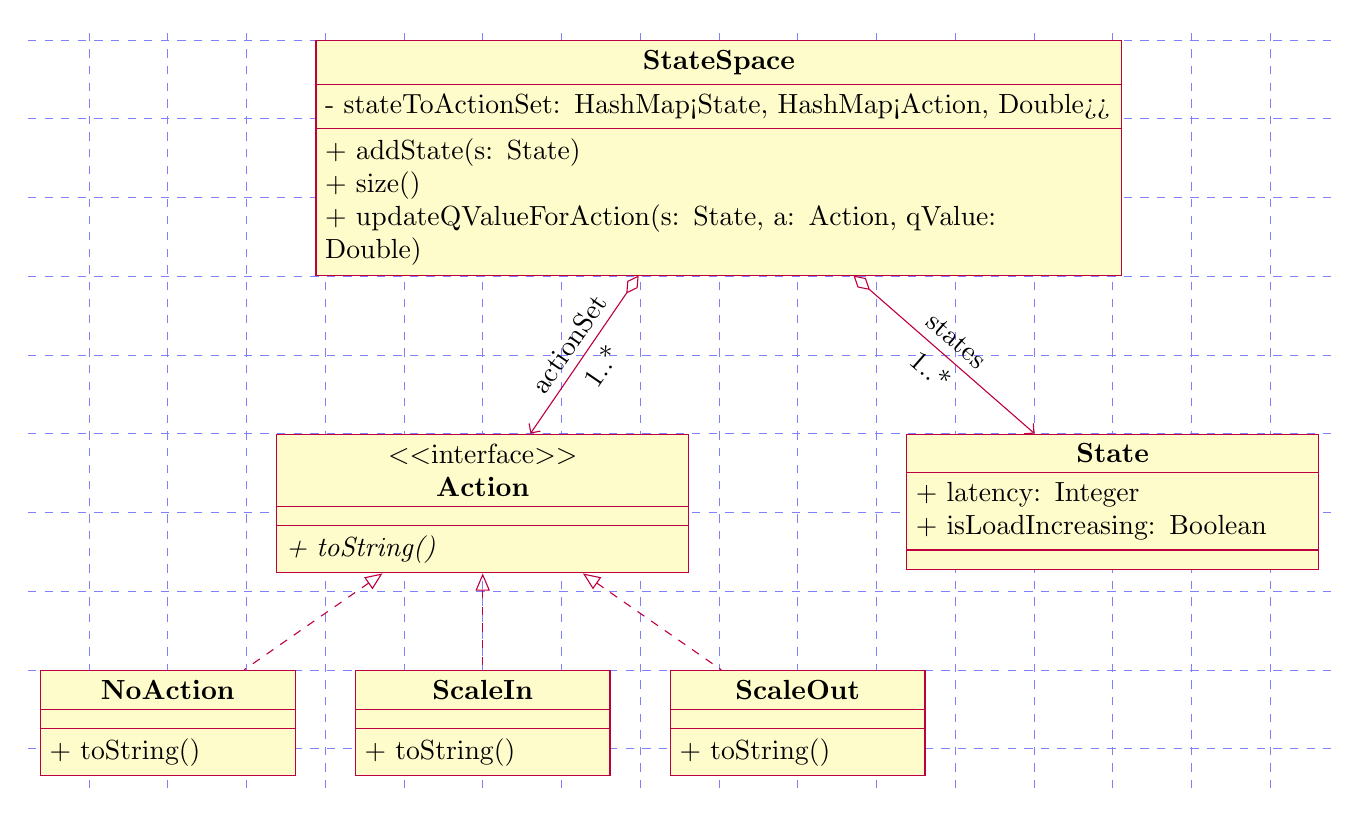
\begin{tikzpicture}[show background grid]
    \begin{class}[text width=10cm]{StateSpace}{7,0}
        \attribute{- stateToActionSet: HashMap<State, HashMap<Action, Double>{}>}
        \operation{+ addState(s: State)}
        \operation{+ size()}
        \operation{+ updateQValueForAction(s: State, a: Action, qValue: Double)}
    \end{class}
    \begin{class}{State}{12,-5}
        \attribute{+ latency: Integer}
        \attribute{+ isLoadIncreasing: Boolean}
    \end{class}
    \begin{interface}{Action}{4,-5}
        \operation[0]{+ toString()}
    \end{interface}
    \begin{class}[text width=3cm]{NoAction}{0,-8}
        \implement{Action}
        \operation{+ toString()}
    \end{class}
    \begin{class}[text width=3cm]{ScaleIn}{4,-8}
        \implement{Action}
        \operation{+ toString()}
    \end{class}
    \begin{class}[text width=3cm]{ScaleOut}{8,-8}
        \implement{Action}
        \operation{+ toString()}
    \end{class}
    
    \aggregation{StateSpace}{}{}{State}
    \aggregation{StateSpace}{}{}{Action}
    
    \path (StateSpace) -- (State) node[midway,sloped,above]{states}
    node[midway,sloped,below] {1..*};
    \path (StateSpace) -- (Action) node[midway,sloped,above]{actionSet}
    node[midway,sloped,below] {1..*};
    \end{tikzpicture}
    \caption{State Space Class Diagram}
    \label{des:l:state-space}
\end{figure}

\subsection{State Space Initialization}

\clearpage
\section{Configuration}
\label{des:conf}

\section{Conclusion}
\label{des:conc}
\chapter{Evaluation}
\label{eval}
In this chapter the two implemented techniques will be evaluated under three read world workloads. In order to show the effect of each configuration parameter, multiple experiments have been designed and deployed. Table~\ref{des:tab:config} defines the configuration space. First, characteristics of workload will be discussed in Section~\ref{eval:workload}. Thereafter, there is separate section for each experiment.

\section{Workload Characteristic}
\label{eval:workload}

DEBS 2014~\cite{debs2014} has been chosen as a real world workload to test the implementation. Each workload contains data from a random location of the original workload and replayed to feed Spark cluster. All experiments were run for one hour. Figure~\ref{eval:fig:workload} shows distribution of messages in two workloads which have been captured from Spark UI.
\begin{figure}[!htbp]
    \centering
      \begin{subfigure}[h]{\linewidth}
        \centering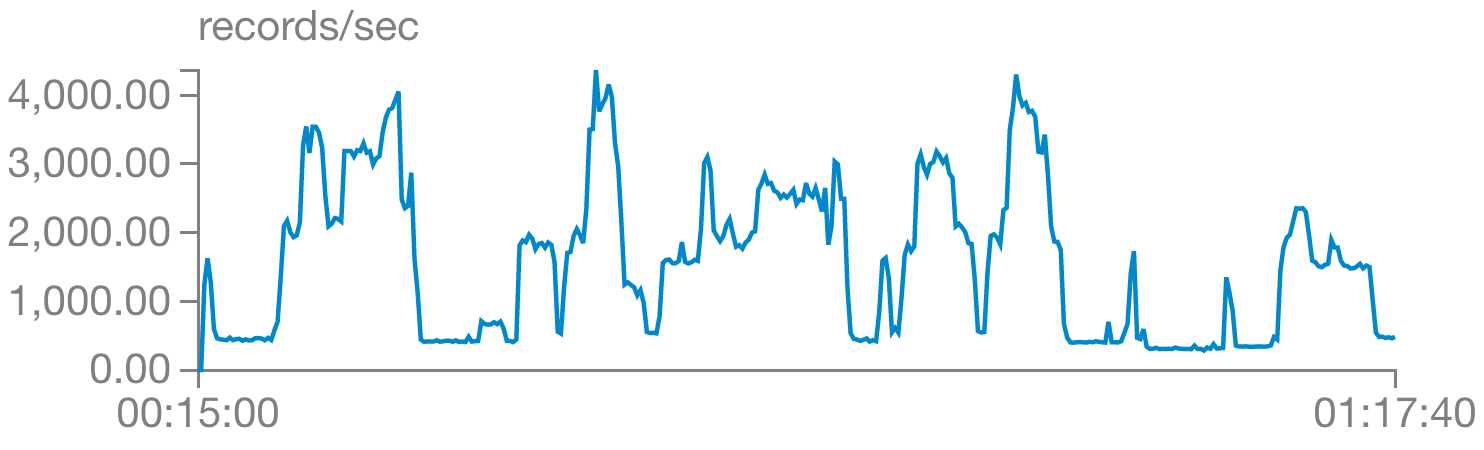
\includegraphics[scale=0.6]{workload1.png}
        \caption{Workload 1}
    \end{subfigure}
    \begin{subfigure}[h]{\linewidth}
        \centering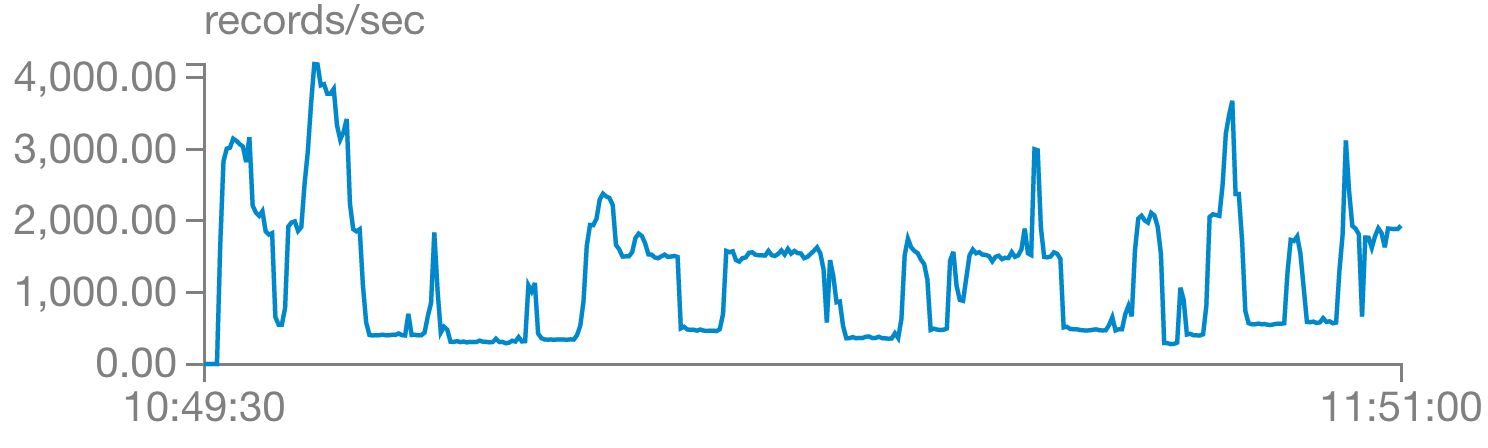
\includegraphics[scale=0.6]{workload2.png}
        \caption{Workload 2}
    \end{subfigure}
    \caption{Two Workloads of DEBS 2014}
    \label{eval:fig:workload}
\end{figure}

The workload involves sensors that measure energy consumption of devices. Each device is connected to one household which in turn is located in one house. This creates a hierarchy from house as parent of households and household as parent of devices. The workload asks to predict energy consumption per device, per household, and per house  for next window of time. The prediction runs over a sliding window of historical measurements which contains $n$ elements. Assuming $window$ variable contains $n$ elements of the history, Equation~\ref{eval:l:pred} defines how the predicted value is calculated.
\begin{equation}
\text{predicted value} = \frac{\text{average(window)} + \text{median(window)}}{2}
\label{eval:l:pred}
\end{equation}

Note that intensity of the workload does not solely depend on number of incoming messages. It also depends on uniqueness of device IDs. A unique device ID inside a micro batch leads to recalculation of Equation~\ref{eval:l:pred} which on its own depends on sort operation to calculate median value. That is, the following cases might occur in one micro batch:
\begin{itemize}
    \item Number of incoming messages is high and uniqueness of devices is also high.
    \item Number if incoming messages is high but uniqueness of devices is low.
    \item Number of incoming messages is low but uniqueness of devices is high.
    \item Number of incoming messages is low and uniqueness of devices is also low.
\end{itemize}
As an example, consider these two batches:
\begin{enumerate}
    \item \label{eval:wl-ex1} A batch of 500 records belonging to 500 hundred devices -- one record for each device -- which leads to 500 sort operations. Bare in mind that, it is \emph{not} 500 hundred sort operation on a 1-element list. Each record is accumulated with previous records of the sliding window and then sorted.
    \item \label{eval:wl-ex2} A batch of 2000 records belonging to 5 devices -- 400 hundred records for each device -- which leads to 5 sort operations.
\end{enumerate}
Case~\ref{eval:wl-ex1} is much more CPU intensive than case~\ref{eval:wl-ex2}. In order to make each workload CPU intensive enough, window size is changed for each workload. Table~\ref{eval:tab:history} defines the history window size for each workload.
\begin{table}[h]
    \begin{tabular}{lc}
        \toprule
        \textbf{Workload} & \textbf{Window Size = $n$ }\\
        \midrule
        Workload 1 & 1650\\
        Workload 2 & 1900\\
        \bottomrule
    \end{tabular}
    \centering
    \caption{Workload Window Size}
    \label{eval:tab:history}
\end{table}

In all experiments \emph{batch size} is set to 10 seconds. The cluster uses 24 executors with minimum of 4 executors that should be respected by Auto-Scaler. All experiments start with minimum number of executors -- 4 in this case -- and run for \emph{one} hour. In case any training is required to run the experiment, training data set is separated from the original workload dataset. In all experiments -- except the last one -- four charts are illustrated. Two charts for latency and two charts for number of executors. Candlestick charts depicts minimum, 10 percentile, average, 90 percentile and maximum values. Furthermore, all experiments were run \emph{two} times and the average of them is included in charts.

\clearpage
\section{Experiment 1: Executor Strategy}
This experiment has been designed to illustrate the strategy of adding/removing executors when taking Scale-In or Scale-Out actions. Table~\ref{eval:tab:ex1} shows the configuration of this experiment.
\begin{table}[h]
    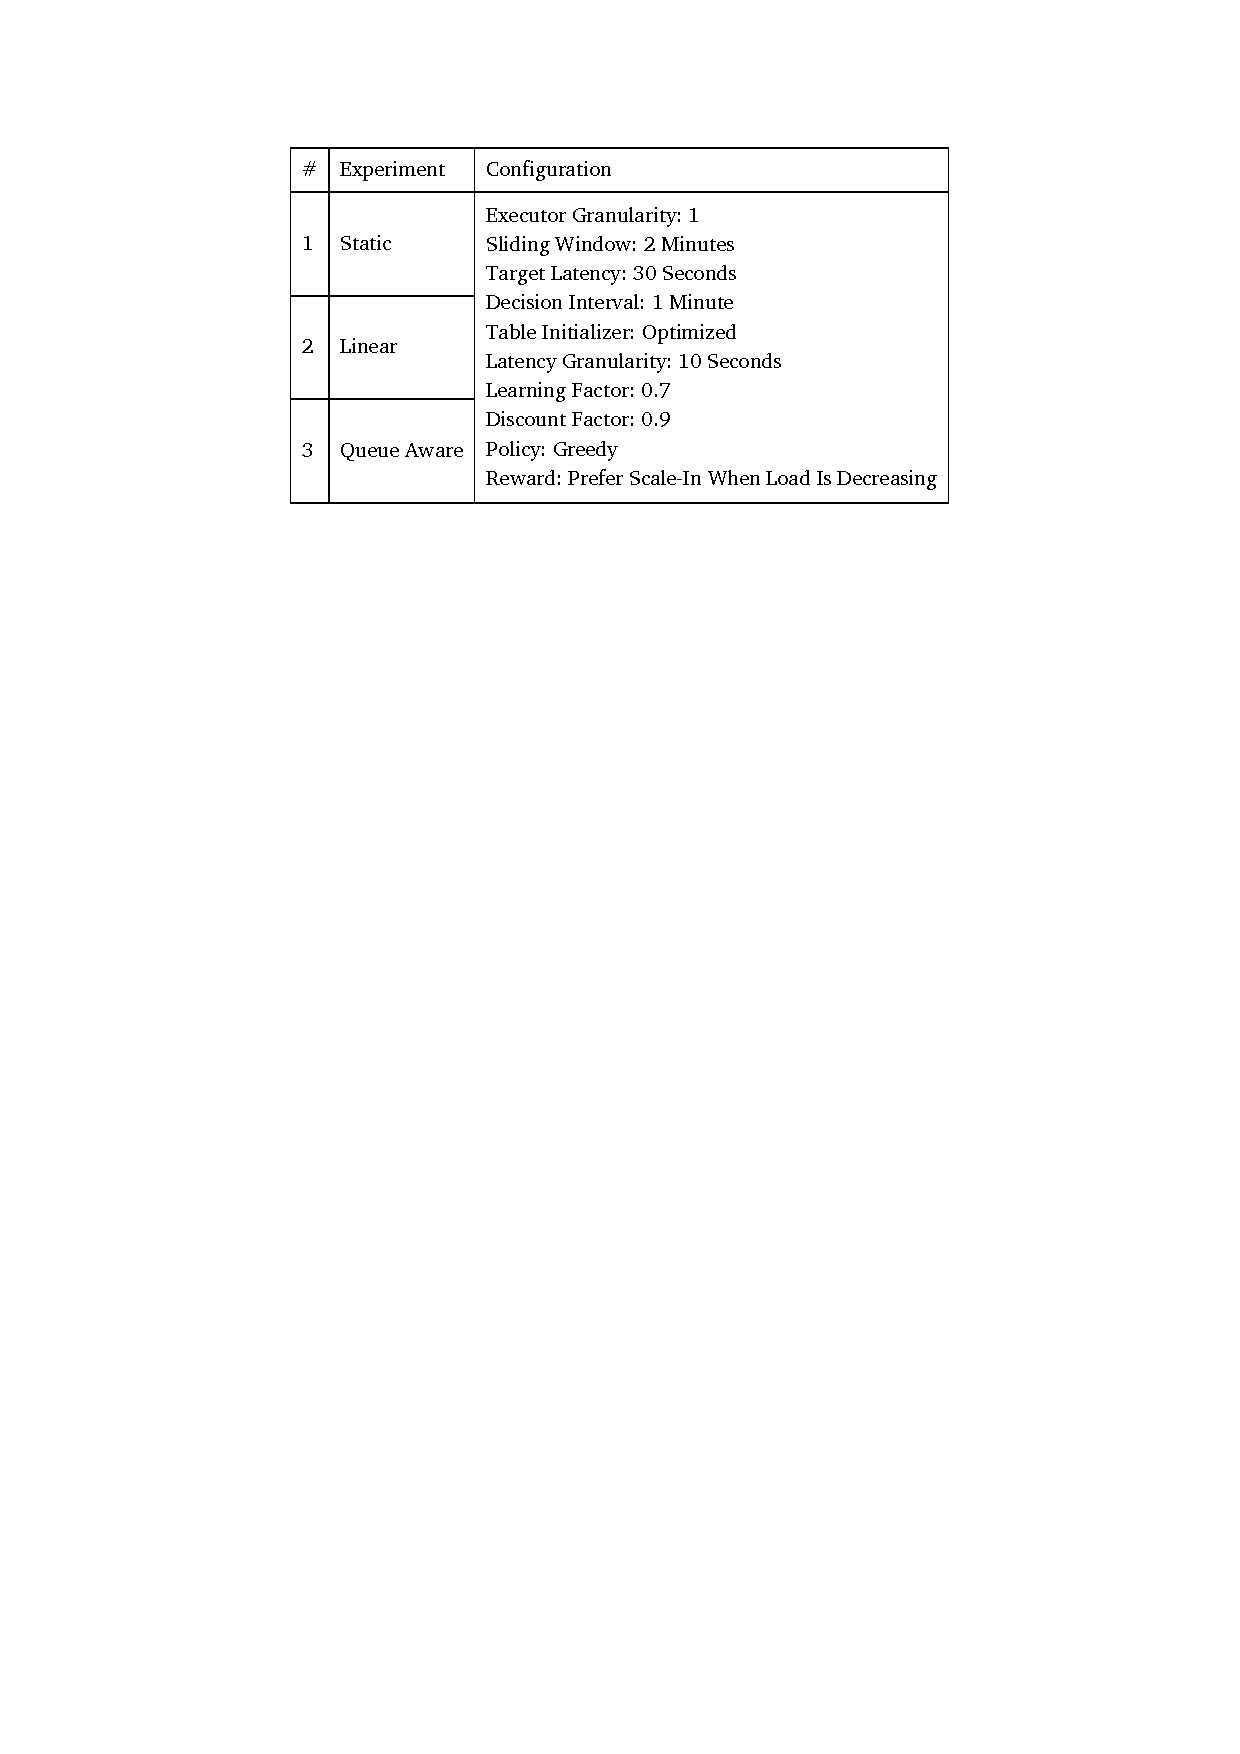
\includegraphics[clip,trim=3.6cm 21.18cm 2.75cm 2.5cm]{tables/ex1.pdf}
    \centering
    \caption{Executor Strategy Configuration Parameters}
    \label{eval:tab:ex1}
\end{table}

Figure~\ref{eval:f:e1:w1:lat},~\ref{eval:f:e1:w1:lat-c} depicts latency charts for first workload. Furthermore, Figure~\ref{eval:f:e1:w1:exec},~\ref{eval:f:e1:w1:exec-c} depicts the behavior of strategies regarding number of executors. Similarity, Figure~\ref{eval:f:e1:w2:lat},~\ref{eval:f:e1:w2:lat-c},~\ref{eval:f:e1:w2:exec} and~\ref{eval:f:e1:w2:exec-c} illustrates latency and executor charts for second workload.

\begin{figure}[!htbp]
\centering
\begin{gnuplot}[terminal=epslatex, terminaloptions=color colortext]
set terminal epslatex size 16cm,7.5cm
set key outside center top horizontal
set datafile separator ';'
set xdata time
set timefmt '%H:%M:%S'
set xr ['0:00:00':'1:00:00']
set yr [0:150]
set xtics '00:00:00',600 nomirror
set ytics 0,30 nomirror
set y2r [0:150]
set y2tics 0,30
set samples 50000 
unset mxtics
unset mytics
set grid ytics lc rgb "#bbbbbb" lw 1 lt 0
set grid xtics lc rgb "#bbbbbb" lw 1 lt 0
unset xl
set yl 'Latency (Seconds)'
plot 'ex/e1/w1/latency.csv' using 1:2 w l lc 'red' lw 4 smooth csplines t 'Static',\
'' using 1:3 w l lc 'blue' lw 4 smooth csplines t 'Linear',\
'' using 1:4 w l lc 'black' lw 4 smooth csplines t 'Q-Aware'
\end{gnuplot}
\caption{Executor Strategy -- Workload 1 -- Latency}
\label{eval:f:e1:w1:lat}
\end{figure}
\begin{figure}[!htbp]
	\centering
	\begin{minipage}[h]{\linewidth}
		\centering
		\begin{gnuplot}[terminal=epslatex, terminaloptions=color colortext]
			set terminal epslatex size 16cm,7.5cm
			set key outside center top horizontal
			set datafile separator ';'
            set key width -12
			set xr [0.5:3.5]
			set yr [0:150]
			set ytics 0,30 nomirror
			set y2r [0:150]
			set y2tics 0,30 nomirror
			set boxwidth 0.3 absolute
			set style fill empty
			unset xl
            set grid ytics lc rgb "#bbbbbb" lw 1 lt 0
            set grid xtics lc rgb "#bbbbbb" lw 1 lt 0
			set yl 'Latency (Seconds)'
			plot 'ex/e1/w1/latency-c.csv' using 1:2:3:4:5:xticlabels(7) with candlesticks lc 'black' lw 4 t 'Min/Max/Percentiles',\
			'' using 1:6:6:6:6 with linespoints pt 5 lc 'black' lw 4 t 'Average',\
            30 dashtype 2 lc 'black' lw 4 t 'Target'
		\end{gnuplot}
		\caption{Executor Strategy -- Workload 1 -- Latency}
		\label{eval:f:e1:w1:lat-c}
	\end{minipage}\hfil
	\begin{minipage}[h]{\linewidth}
		\centering
		\begin{gnuplot}[terminal=epslatex, terminaloptions=color colortext]
			set terminal epslatex size 16cm,7.5cm
			set key outside center top horizontal
			set datafile separator ';'
			set xdata time
			set timefmt '%H:%M:%S'
			set xr ['0:00:00':'1:00:00']
			set yr [2:26]
			set y2r [2:26]
			set ytics 0,4 nomirror
			set xtics '00:00:00',600 nomirror
			set y2tics 0,4
			unset mxtics
			unset mytics
			unset xl
            set grid ytics lc rgb "#bbbbbb" lw 1 lt 0
            set grid xtics lc rgb "#bbbbbb" lw 1 lt 0
			set yl 'Number of Executors'
			plot 'ex/e1/w1/exec.csv' using 1:2 w l lc 'red' lw 4 t 'Static',\
			'' using 1:3 w l lc 'blue' lw 4 t 'Linear',\
			'' using 1:4 w l lc 'black' lw 4 t 'Q-Aware'
		\end{gnuplot}
		\caption{Executor Strategy -- Workload 1 -- Number of Executors}
		\label{eval:f:e1:w1:exec}
	\end{minipage}\hfil
	\begin{minipage}[h]{\linewidth}
		\centering
		\begin{gnuplot}[terminal=epslatex, terminaloptions=color colortext]
			set terminal epslatex size 16cm,7.5cm
			set key outside center top horizontal
			set datafile separator ';'
			set xr [0.5:3.5]
			set yr [2:26]
			set y2r [2:26]
			set ytics 0,4 nomirror
			set y2tics 0,4 nomirror
			set boxwidth 0.3 absolute
			set style fill empty
			unset xl
            set grid ytics lc rgb "#bbbbbb" lw 1 lt 0
            set grid xtics lc rgb "#bbbbbb" lw 1 lt 0
			set yl 'Number of Executors'
			plot 'ex/e1/w1/exec-c.csv' using 1:2:3:4:5:xticlabels(7) with candlesticks lc 'black' lw 4 t 'Min/Max/Percentiles',\
			'' using 1:6:6:6:6 with linespoints pt 5 lc 'black' lw 4 t 'Average' 
		\end{gnuplot}
		\caption{Executor Strategy -- Workload 1 -- Number of Executors}
		\label{eval:f:e1:w1:exec-c}
	\end{minipage}
\end{figure}
\begin{figure}[!htbp]
	\centering
	\begin{minipage}[h]{\linewidth}
		\centering
		\begin{gnuplot}[terminal=epslatex, terminaloptions=color colortext]
			set terminal epslatex size 16cm,7.5cm
			set key outside center top horizontal
			set datafile separator ';'
			set xdata time
			set timefmt '%H:%M:%S'
			set xr ['0:00:00':'1:00:00']
			set yr [0:170]
			set y2r [0:170]
			set xtics '00:00:00',600 nomirror
			set ytics 0,30 nomirror
			set y2tics 0,30
			unset mxtics
			unset mytics
			set samples 50000 
			unset xl
            set grid ytics lc rgb "#bbbbbb" lw 1 lt 0
            set grid xtics lc rgb "#bbbbbb" lw 1 lt 0
			set yl 'Latency (Seconds)'
			plot 'ex/e1/w2/latency.csv' using 1:2 w l lc 'red' lw 4 smooth csplines t 'Static',\
			'' using 1:3 w l lc 'blue' lw 4 smooth csplines t 'Linear',\
			'' using 1:4 w l lc 'black' lw 4 smooth csplines t 'Q-Aware'
		\end{gnuplot}
		\caption{Executor Strategy -- Workload 2 -- Latency}
		\label{eval:f:e1:w2:lat}
	\end{minipage}\hfil
	\begin{minipage}[h]{\linewidth}
		\centering
		\begin{gnuplot}[terminal=epslatex, terminaloptions=color colortext]
			set terminal epslatex size 16cm,7.5cm
			set key outside center top horizontal
			set datafile separator ';'
            set key width -12
			set xr [0.5:3.5]
			set yr [0:170]
			set y2r [0:170]
			set ytics 0,30 nomirror
			set y2tics 0,30 nomirror
			set boxwidth 0.3 absolute
			set style fill empty
			unset xl
            set grid ytics lc rgb "#bbbbbb" lw 1 lt 0
            set grid xtics lc rgb "#bbbbbb" lw 1 lt 0
			set yl 'Latency (Seconds)'
			plot 'ex/e1/w2/latency-c.csv' using 1:2:3:4:5:xticlabels(7) with candlesticks lc 'black' lw 4 t 'Min/Max/Percentiles',\
			'' using 1:6:6:6:6 with linespoints pt 5 lc 'black' lw 4 t 'Average',\
            30 dashtype 2 lc 'black' lw 4 t 'Target'
		\end{gnuplot}
		\caption{Executor Strategy -- Workload 2 -- Latency}
		\label{eval:f:e1:w2:lat-c}
	\end{minipage}\hfil
	\begin{minipage}[h]{\linewidth}
		\centering
		\begin{gnuplot}[terminal=epslatex, terminaloptions=color colortext]
			set terminal epslatex size 16cm,7.5cm
			set key outside center top horizontal
			set datafile separator ';'
			set xdata time
			set timefmt '%H:%M:%S'
			set xr ['0:00:00':'1:00:00']
			set yr [2:26]
			set y2r [2:26]
			set xtics '00:00:00',600 nomirror
			set ytics 0,4 nomirror
			set y2tics 0,4
			unset mxtics
			unset mytics
			unset xl
            set grid ytics lc rgb "#bbbbbb" lw 1 lt 0
            set grid xtics lc rgb "#bbbbbb" lw 1 lt 0
			set yl 'Number of Executors'
			plot 'ex/e1/w2/exec.csv' using 1:2 w l lc 'red' lw 4 t 'Static',\
			'' using 1:3 w l lc 'blue' lw 4 t 'Linear',\
			'' using 1:4 w l lc 'black' lw 4 t 'Q-Aware'
		\end{gnuplot}
		\caption{Executor Strategy -- Workload 2 -- Number of Executors}
		\label{eval:f:e1:w2:exec}
	\end{minipage}
\end{figure}
\begin{figure}[!htbp]
\centering
\begin{gnuplot}[terminal=epslatex, terminaloptions=color colortext]
set terminal epslatex size 16cm,7.5cm
set key outside center top horizontal
set datafile separator ';'
set xr [0.5:3.5]
set yr [2:26]
set ytics 0,4 nomirror
set y2r [2:26]
set y2tics 0,4 nomirror
set boxwidth 0.3 absolute
set style fill empty
unset xl
set grid ytics lc rgb "#bbbbbb" lw 1 lt 0
set grid xtics lc rgb "#bbbbbb" lw 1 lt 0
set yl 'Number of Executors'
plot 'ex/e1/w2/exec-c.csv' using 1:2:3:4:5:xticlabels(7) with candlesticks lc 'black' lw 4 t 'Min/Max/Percentiles','' using 1:6:6:6:6 with linespoints pt 5 lc 'black' lw 4 t 'Average' 
\end{gnuplot}
\caption{Executor Strategy -- Workload 2 -- Number of Executors}
\label{eval:f:e1:w2:exec-c}
\end{figure}
\FloatBarrier
\subsection{Conclusion}
As depicted in last section, for Workload 1, Static strategy performs slightly better than Queue Aware strategy. Both of them were able reach target latency to some degree, though they are still above target latency. However, for Workload 2 Queue Aware strategy outperforms all other strategies, since Static and Linear strategies violate target latency.

It can be speculated that Queue Aware strategy is the best strategy amongst three strategies. However, it can't be proven now. More experiments shall be done. Thus, for next set of experiments Queue Aware strategy is chosen to be evaluated extensively. Furthermore, the conclusion is only based on two workloads and it can't be generalized.
\clearpage
\section{Experiment 2: History Window}
This experiment has been designed to illustrate the effect of history window on quality of decision made by Auto-Scaler. Table~\ref{eval:tab:ex2} shows the configuration of this experiment.
\begin{table}[h]
    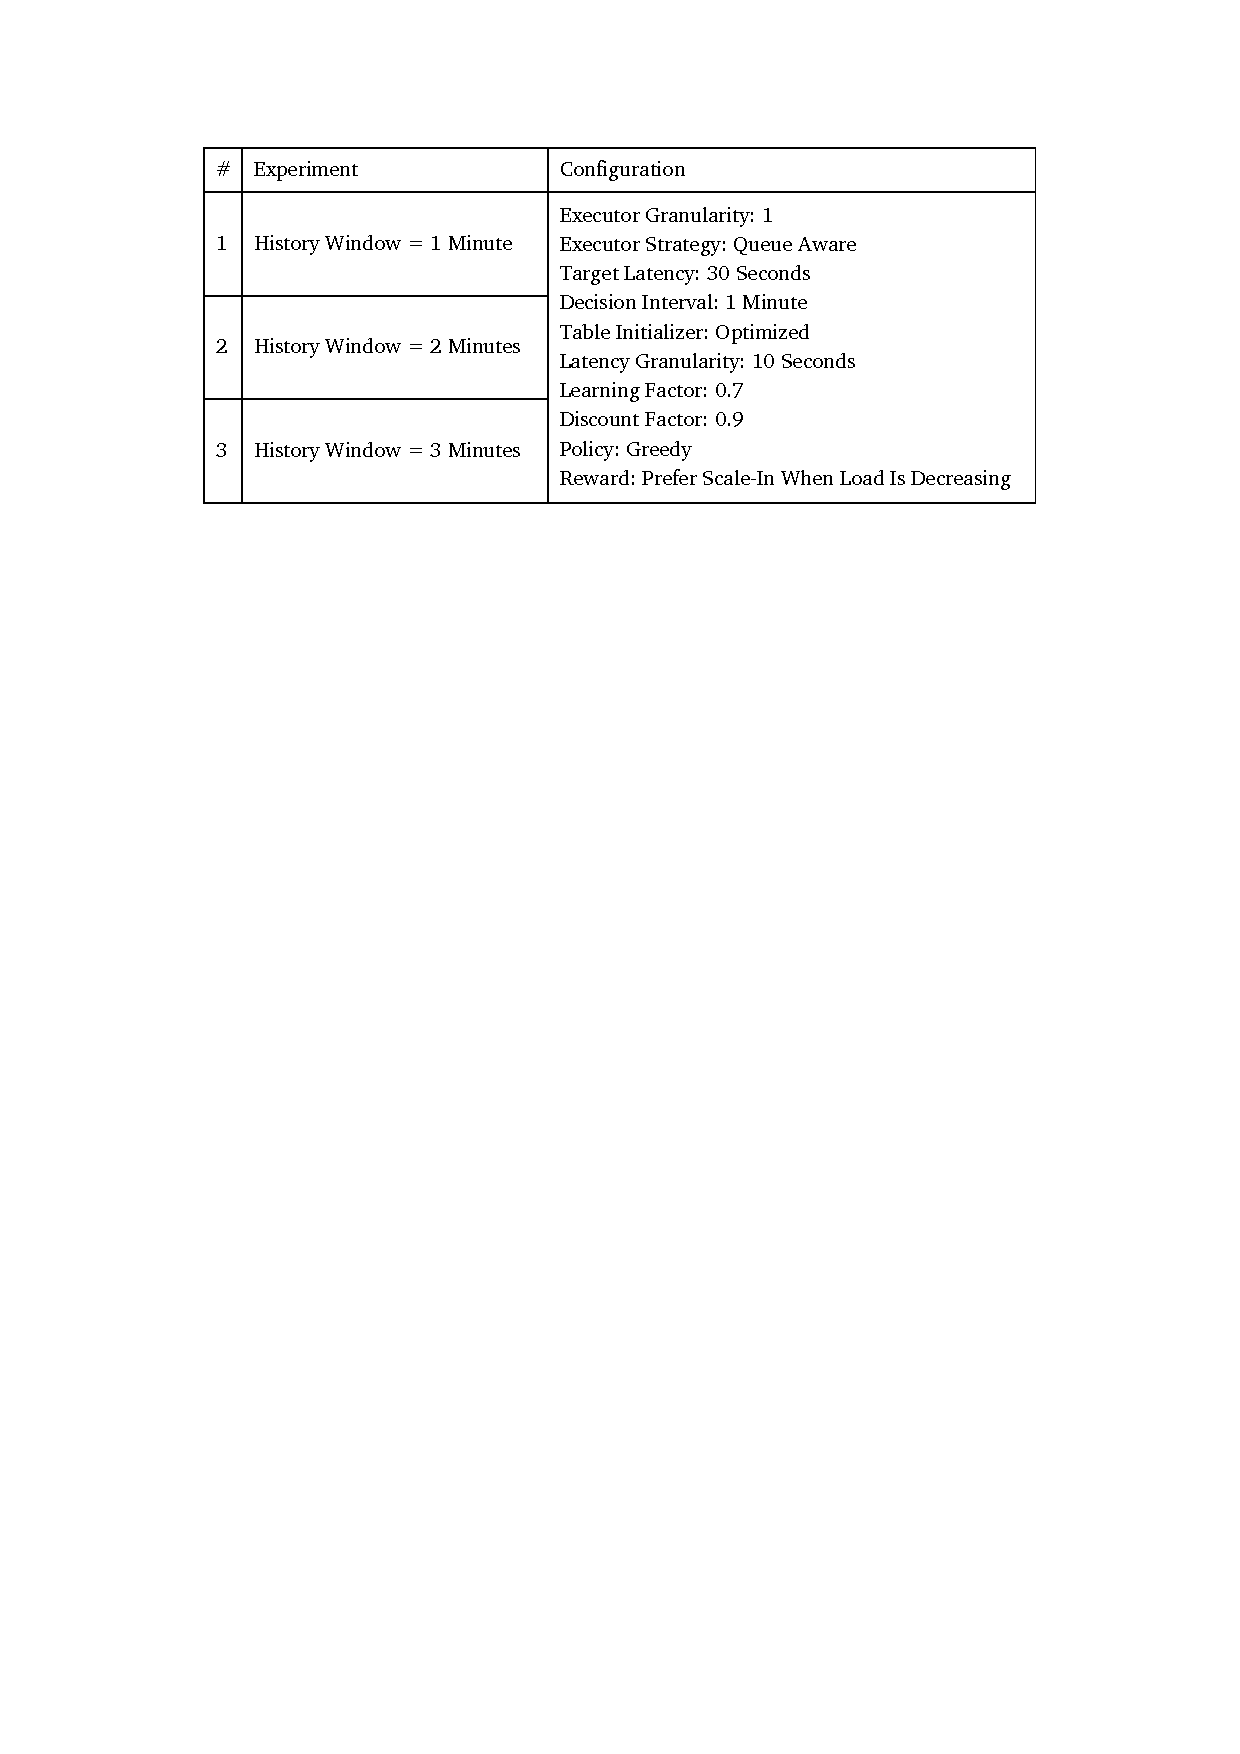
\includegraphics[clip,trim=3.3cm 21.18cm 3.25cm 2.5cm]{tables/ex2.pdf}
    \centering
    \caption{History Window Configuration Parameters}
    \label{eval:tab:ex2}
\end{table}

Figures~\ref{eval:f:e2:w1:lat},~\ref{eval:f:e2:w1:lat-c},~\ref{eval:f:e2:w1:exec} and ~\ref{eval:f:e2:w1:exec-c} illustrates latency and executor charts for Workload 1. Figures~\ref{eval:f:e2:w2:lat},~\ref{eval:f:e2:w2:lat-c},~\ref{eval:f:e2:w2:exec} and~\ref{eval:f:e2:w2:exec-c} illustrates latency and executor charts for Workload 2.

\begin{figure}[!htbp]
    \centering
    \begin{gnuplot}[terminal=epslatex, terminaloptions=color colortext]
        set terminal epslatex size 16cm,7.5cm
        set key outside center top horizontal
        set datafile separator ';'
        set xdata time
        set timefmt '%H:%M:%S'
        set xr ['0:00:00':'1:00:00']
        set yr [0:120]
        set xtics '00:00:00',600 nomirror
        set ytics 0,30 nomirror
        set y2r [0:120]
        set y2tics 0,30 nomirror
        set samples 50000 
        unset mxtics
        unset mytics
        unset xl
        set grid ytics lc rgb "#bbbbbb" lw 1 lt 0
        set grid xtics lc rgb "#bbbbbb" lw 1 lt 0
        set yl 'Latency (Seconds)'
        plot 'ex/e2/w1/latency.csv' using 1:2 w l lc 'red' lw 4 smooth csplines t '1 Min',\
        '' using 1:3 w l lc 'blue' lw 4 smooth csplines t '2 Min',\
        '' using 1:4 w l lc 'black' lw 4 smooth csplines t '3 Min'
    \end{gnuplot}
    \caption{History Window -- Workload 1 -- Latency}
    \label{eval:f:e2:w1:lat}
\end{figure}
\begin{figure}[!htbp]
    \centering
    \begin{minipage}[h]{\linewidth}
        \centering
        \begin{gnuplot}[terminal=epslatex, terminaloptions=color colortext]
            set terminal epslatex size 16cm,7.5cm
            set key outside center top horizontal
            set datafile separator ';'
            set key width -12
            set xr [0.5:3.5]
            set yr [0:120]
            set ytics 0,30 nomirror
            set y2r [0:120]
            set y2tics 0,30 nomirror
            set boxwidth 0.3 absolute
            set style fill empty
            unset xl
            set grid ytics lc rgb "#bbbbbb" lw 1 lt 0
            set grid xtics lc rgb "#bbbbbb" lw 1 lt 0
            set yl 'Latency (Seconds)'
            plot 'ex/e2/w1/latency-c.csv' using 1:2:3:4:5:xticlabels(7) with candlesticks lc 'black' lw 4 t 'Min/Max/Percentiles',\
            '' using 1:6:6:6:6 with linespoints pt 5 lc 'black' lw 4 t 'Average',\
            30 dashtype 2 lc 'black' lw 4 t 'Target'
        \end{gnuplot}
        \caption{History Window -- Workload 1 -- Latency}
        \label{eval:f:e2:w1:lat-c}
    \end{minipage}\hfil
    \begin{minipage}[h]{\linewidth}
        \centering
        \begin{gnuplot}[terminal=epslatex, terminaloptions=color colortext]
            set terminal epslatex size 16cm,7.5cm
            set key outside center top horizontal
            set datafile separator ';'
            set xdata time
            set timefmt '%H:%M:%S'
            set xr ['0:00:00':'1:00:00']
            set yr [2:26]
            set y2r [2:26]
            set ytics 0,4 nomirror
            set xtics '00:00:00',600 nomirror
            set y2tics 0,4 nomirror
            unset mxtics
            unset mytics
            unset xl
            set grid ytics lc rgb "#bbbbbb" lw 1 lt 0
            set grid xtics lc rgb "#bbbbbb" lw 1 lt 0
            set yl 'Number of Executors'
            plot 'ex/e2/w1/exec.csv' using 1:2 w l lc 'red' lw 4 t '1 Min',\
            '' using 1:3 w l lc 'blue' lw 4 t '2 Min',\
            '' using 1:4 w l lc 'black' lw 4 t '3 Min'
        \end{gnuplot}
        \caption{History Window -- Workload 1 -- Number of Executors}
        \label{eval:f:e2:w1:exec}
    \end{minipage}\hfil
    \begin{minipage}[h]{\linewidth}
        \centering
        \begin{gnuplot}[terminal=epslatex, terminaloptions=color colortext]
            set terminal epslatex size 16cm,7.5cm
            set key outside center top horizontal
            set datafile separator ';'
            set xr [0.5:3.5]
            set yr [2:26]
            set y2r [2:26]
            set ytics 0,4 nomirror
            set y2tics 0,4 nomirror
            set boxwidth 0.3 absolute
            set style fill empty
            unset xl
            set grid ytics lc rgb "#bbbbbb" lw 1 lt 0
            set grid xtics lc rgb "#bbbbbb" lw 1 lt 0
            set yl 'Number of Executors'
            plot 'ex/e2/w1/exec-c.csv' using 1:2:3:4:5:xticlabels(7) with candlesticks lc 'black' lw 4 t 'Min/Max/Percentiles',\
            '' using 1:6:6:6:6 with linespoints pt 5 lc 'black' lw 4 t 'Average' 
        \end{gnuplot}
        \caption{History Window -- Workload 1 -- Number of Executors}
        \label{eval:f:e2:w1:exec-c}
    \end{minipage}
\end{figure}
\begin{figure}[!htbp]
    \centering
    \begin{minipage}[h]{\linewidth}
        \centering
        \begin{gnuplot}[terminal=epslatex, terminaloptions=color colortext]
            set terminal epslatex size 16cm,7.5cm
            set key outside center top horizontal
            set datafile separator ';'
            set xdata time
            set timefmt '%H:%M:%S'
            set xr ['0:00:00':'1:00:00']
            set yr [0:130]
            set y2r [0:130]
            set xtics '00:00:00',600 nomirror
            set ytics 0,30 nomirror
            set y2tics 0,30 nomirror
            unset mxtics
            unset mytics
            set samples 50000 
            unset xl
            set grid ytics lc rgb "#bbbbbb" lw 1 lt 0
            set grid xtics lc rgb "#bbbbbb" lw 1 lt 0
            set yl 'Latency (Seconds)'
            plot 'ex/e2/w2/latency.csv' using 1:2 w l lc 'red' lw 4 smooth csplines t '1 Min',\
            '' using 1:3 w l lc 'blue' lw 4 smooth csplines t '2 Min',\
            '' using 1:4 w l lc 'black' lw 4 smooth csplines t '3 Min'
        \end{gnuplot}
        \caption{History Window -- Workload 2 -- Latency}
        \label{eval:f:e2:w2:lat}
    \end{minipage}\hfil
    \begin{minipage}[h]{\linewidth}
        \centering
        \begin{gnuplot}[terminal=epslatex, terminaloptions=color colortext]
            set terminal epslatex size 16cm,7.5cm
            set key outside center top horizontal
            set datafile separator ';'
            set key width -12
            set xr [0.5:3.5]
            set yr [0:130]
            set y2r [0:130]
            set ytics 0,30 nomirror
            set y2tics 0,30 nomirror
            set boxwidth 0.3 absolute
            set style fill empty
            unset xl
            set grid ytics lc rgb "#bbbbbb" lw 1 lt 0
            set grid xtics lc rgb "#bbbbbb" lw 1 lt 0
            set yl 'Latency (Seconds)'
            plot 'ex/e2/w2/latency-c.csv' using 1:2:3:4:5:xticlabels(7) with candlesticks lc 'black' lw 4 t 'Min/Max/Percentiles',\
            '' using 1:6:6:6:6 with linespoints pt 5 lc 'black' lw 4 t 'Average',\
            30 dashtype 2 lc 'black' lw 4 t 'Target'
        \end{gnuplot}
        \caption{History Window -- Workload 2 -- Latency}
        \label{eval:f:e2:w2:lat-c}
    \end{minipage}\hfil
    \begin{minipage}[h]{\linewidth}
        \centering
        \begin{gnuplot}[terminal=epslatex, terminaloptions=color colortext]
            set terminal epslatex size 16cm,7.5cm
            set key outside center top horizontal
            set datafile separator ';'
            set xdata time
            set timefmt '%H:%M:%S'
            set xr ['0:00:00':'1:00:00']
            set yr [2:26]
            set y2r [2:26]
            set xtics '00:00:00',600 nomirror
            set ytics 0,4 nomirror
            set y2tics 0,4 nomirror
            unset mxtics
            unset mytics
            unset xl
            set grid ytics lc rgb "#bbbbbb" lw 1 lt 0
            set grid xtics lc rgb "#bbbbbb" lw 1 lt 0
            set yl 'Number of Executors'
            plot 'ex/e2/w2/exec.csv' using 1:2 w l lc 'red' lw 4 t '1 Min',\
            '' using 1:3 w l lc 'blue' lw 4 t '2 Min',\
            '' using 1:4 w l lc 'black' lw 4 t '3 Min'
        \end{gnuplot}
        \caption{History Window -- Workload 2 -- Number of Executors}
        \label{eval:f:e2:w2:exec}
    \end{minipage}
\end{figure}
\begin{figure}[!htbp]
    \centering
    \begin{gnuplot}[terminal=epslatex, terminaloptions=color colortext]
        set terminal epslatex size 16cm,7.5cm
        set key outside center top horizontal
        set datafile separator ';'
        set xr [0.5:3.5]
        set yr [2:26]
        set ytics 0,4 nomirror
        set y2r [2:26]
        set y2tics 0,4 nomirror
        set boxwidth 0.3 absolute
        set style fill empty
        unset xl
        set grid ytics lc rgb "#bbbbbb" lw 1 lt 0
        set grid xtics lc rgb "#bbbbbb" lw 1 lt 0
        set yl 'Number of Executors'
        plot 'ex/e2/w2/exec-c.csv' using 1:2:3:4:5:xticlabels(7) with candlesticks lc 'black' lw 4 t 'Min/Max/Percentiles','' using 1:6:6:6:6 with linespoints pt 5 lc 'black' lw 4 t 'Average' 
    \end{gnuplot}
    \caption{History Window -- Workload 2 -- Number of Executors}
    \label{eval:f:e2:w2:exec-c}
\end{figure}
\FloatBarrier
\subsection{Conclusion}
For Workload 1, three-minute history window leads to better latency albeit with slightly more executors. However, for second workload two-minute window outperforms both one and three minute windows.

Also note that, short history window (like one-minute) makes Auto-Scaler too sensitive to noisy workloads. This can be confirmed by Figure~\ref{eval:f:e2:w2:exec}. As depicted, one-minute history window suffers from zig-zag decisions when it reaches 24 executors. Two-minute window to some degree suffers from this issue as well. However, three-minute window is resistant to this issue.

In general, history window of two minutes shows better results than the others. Thus, for rest of the experiments this window size will be used.
\clearpage
\section{Experiment 3: Decision Interval}
The Auto-Scaler implemented in thesis makes decisions in intervals defined by \lstinline|decisionInterval| parameter. This experiment has been designed to illustrate the effect of this parameter on behvaior of the Auto-Scaler. Table~\ref{eval:tab:ex3} shows the configuration of this experiment.
\begin{table}[h]
    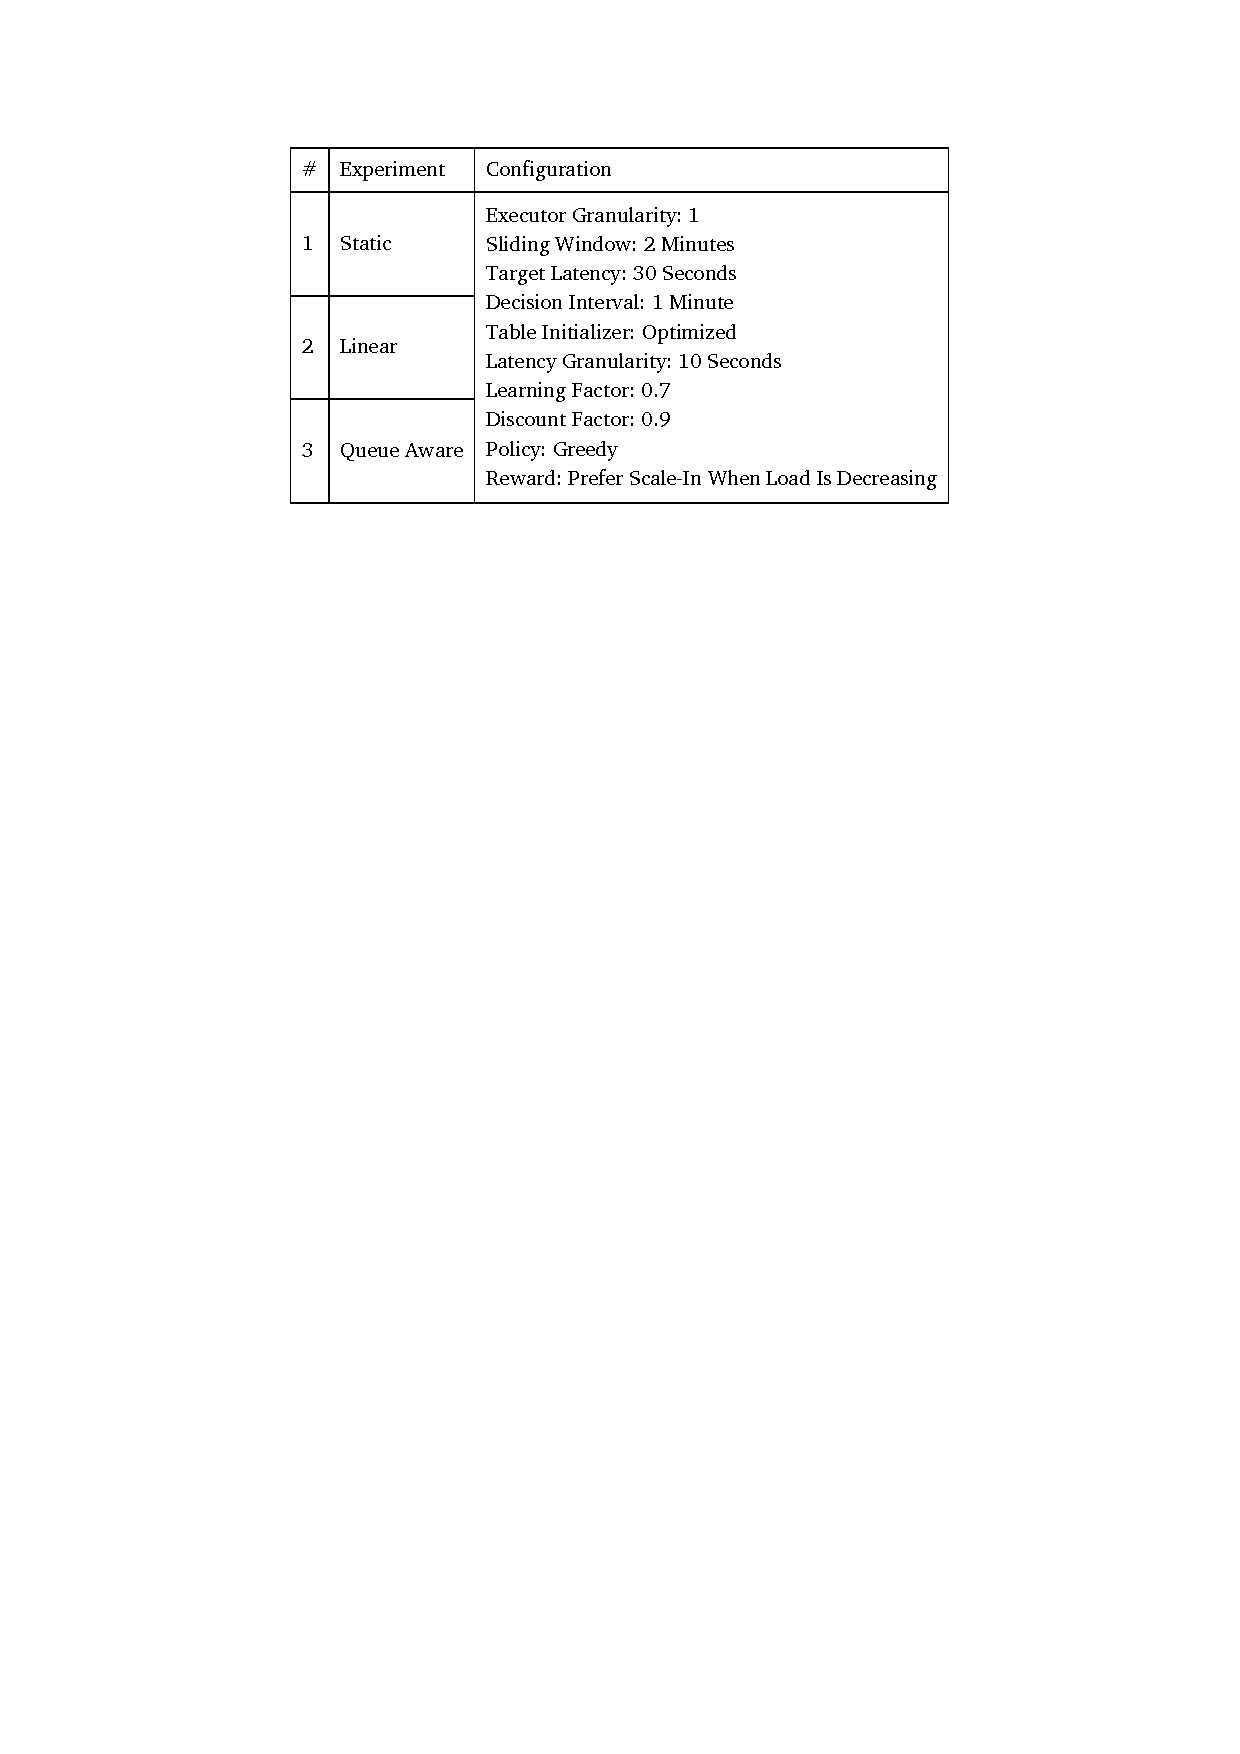
\includegraphics[clip,trim=3.3cm 21.18cm 3.25cm 2.5cm]{tables/ex3.pdf}
    \centering
    \caption{Decision Interval Configuration Parameters}
    \label{eval:tab:ex3}
\end{table}

Figures~\ref{eval:f:e3:w1:lat},~\ref{eval:f:e3:w1:lat-c},~\ref{eval:f:e3:w1:exec} and ~\ref{eval:f:e3:w1:exec-c} illustrates latency and executor charts for Workload 1. Figures~\ref{eval:f:e3:w2:lat},~\ref{eval:f:e3:w2:lat-c},~\ref{eval:f:e3:w2:exec} and~\ref{eval:f:e3:w2:exec-c} illustrates latency and executor charts for Workload 2.

\begin{figure}[!htbp]
    \centering
    \begin{gnuplot}[terminal=epslatex, terminaloptions=color colortext]
        set terminal epslatex size 16cm,7.5cm
        set key outside center top horizontal
        set datafile separator ';'
        set xdata time
        set timefmt '%H:%M:%S'
        set xr ['0:00:00':'1:00:00']
        set yr [0:120]
        set xtics '00:00:00',600 nomirror
        set ytics 0,30 nomirror
        set y2r [0:120]
        set y2tics 0,30 nomirror
        set samples 50000 
        unset mxtics
        unset mytics
        unset xl
        set grid ytics lc rgb "#bbbbbb" lw 1 lt 0
        set grid xtics lc rgb "#bbbbbb" lw 1 lt 0
        set yl 'Latency (Seconds)'
        plot 'ex/e3/w1/latency.csv' using 1:2 w l lc 'red' lw 4 smooth csplines t '1 Min',\
        '' using 1:3 w l lc 'blue' lw 4 smooth csplines t '2 Min',\
        '' using 1:4 w l lc 'black' lw 4 smooth csplines t '3 Min'
    \end{gnuplot}
    \caption{Decision Interval -- Workload 1 -- Latency}
    \label{eval:f:e3:w1:lat}
\end{figure}
\begin{figure}[!htbp]
    \centering
    \begin{minipage}[h]{\linewidth}
        \centering
        \begin{gnuplot}[terminal=epslatex, terminaloptions=color colortext]
            set terminal epslatex size 16cm,7.5cm
            set key outside center top horizontal
            set datafile separator ';'
            set key width -12
            set xr [0.5:3.5]
            set yr [0:120]
            set ytics 0,30 nomirror
            set y2r [0:120]
            set y2tics 0,30 nomirror
            set boxwidth 0.3 absolute
            set style fill empty
            unset xl
            set grid ytics lc rgb "#bbbbbb" lw 1 lt 0
            set grid xtics lc rgb "#bbbbbb" lw 1 lt 0
            set yl 'Latency (Seconds)'
            plot 'ex/e3/w1/latency-c.csv' using 1:2:3:4:5:xticlabels(7) with candlesticks lc 'black' lw 4 t 'Min/Max/Percentiles',\
            '' using 1:6:6:6:6 with linespoints pt 5 lc 'black' lw 4 t 'Average',\
            30 dashtype 2 lc 'black' lw 4 t 'Target'
        \end{gnuplot}
        \caption{Decision Interval -- Workload 1 -- Latency}
        \label{eval:f:e3:w1:lat-c}
    \end{minipage}\hfil
    \begin{minipage}[h]{\linewidth}
        \centering
        \begin{gnuplot}[terminal=epslatex, terminaloptions=color colortext]
            set terminal epslatex size 16cm,7.5cm
            set key outside center top horizontal
            set datafile separator ';'
            set xdata time
            set timefmt '%H:%M:%S'
            set xr ['0:00:00':'1:00:00']
            set yr [2:26]
            set y2r [2:26]
            set ytics 0,4 nomirror
            set xtics '00:00:00',600 nomirror
            set y2tics 0,4 nomirror
            unset mxtics
            unset mytics
            unset xl
            set grid ytics lc rgb "#bbbbbb" lw 1 lt 0
            set grid xtics lc rgb "#bbbbbb" lw 1 lt 0
            set yl 'Number of Executors'
            plot 'ex/e3/w1/exec.csv' using 1:2 w l lc 'red' lw 4 t '1 Min',\
            '' using 1:3 w l lc 'blue' lw 4 t '2 Min',\
            '' using 1:4 w l lc 'black' lw 4 t '3 Min'
        \end{gnuplot}
        \caption{Decision Interval -- Workload 1 -- Number of Executors}
        \label{eval:f:e3:w1:exec}
    \end{minipage}\hfil
    \begin{minipage}[h]{\linewidth}
        \centering
        \begin{gnuplot}[terminal=epslatex, terminaloptions=color colortext]
            set terminal epslatex size 16cm,7.5cm
            set key outside center top horizontal
            set datafile separator ';'
            set xr [0.5:3.5]
            set yr [2:26]
            set y2r [2:26]
            set ytics 0,4 nomirror
            set y2tics 0,4 nomirror
            set boxwidth 0.3 absolute
            set style fill empty
            unset xl
            set grid ytics lc rgb "#bbbbbb" lw 1 lt 0
            set grid xtics lc rgb "#bbbbbb" lw 1 lt 0
            set yl 'Number of Executors'
            plot 'ex/e3/w1/exec-c.csv' using 1:2:3:4:5:xticlabels(7) with candlesticks lc 'black' lw 4 t 'Min/Max/Percentiles',\
            '' using 1:6:6:6:6 with linespoints pt 5 lc 'black' lw 4 t 'Average' 
        \end{gnuplot}
        \caption{Decision Interval -- Workload 1 -- Number of Executors}
        \label{eval:f:e3:w1:exec-c}
    \end{minipage}
\end{figure}
\begin{figure}[!htbp]
    \centering
    \begin{minipage}[h]{\linewidth}
        \centering
        \begin{gnuplot}[terminal=epslatex, terminaloptions=color colortext]
            set terminal epslatex size 16cm,7.5cm
            set key outside center top horizontal
            set datafile separator ';'
            set xdata time
            set timefmt '%H:%M:%S'
            set xr ['0:00:00':'1:00:00']
            set yr [0:120]
            set y2r [0:120]
            set xtics '00:00:00',600 nomirror
            set ytics 0,30 nomirror
            set y2tics 0,30 nomirror
            unset mxtics
            unset mytics
            set samples 50000 
            unset xl
            set grid ytics lc rgb "#bbbbbb" lw 1 lt 0
            set grid xtics lc rgb "#bbbbbb" lw 1 lt 0
            set yl 'Latency (Seconds)'
            plot 'ex/e3/w2/latency.csv' using 1:2 w l lc 'red' lw 4 smooth csplines t '1 Min',\
            '' using 1:3 w l lc 'blue' lw 4 smooth csplines t '2 Min',\
            '' using 1:4 w l lc 'black' lw 4 smooth csplines t '3 Min'
        \end{gnuplot}
        \caption{Decision Interval -- Workload 2 -- Latency}
        \label{eval:f:e3:w2:lat}
    \end{minipage}\hfil
    \begin{minipage}[h]{\linewidth}
        \centering
        \begin{gnuplot}[terminal=epslatex, terminaloptions=color colortext]
            set terminal epslatex size 16cm,7.5cm
            set key outside center top horizontal
            set datafile separator ';'
            set key width -12
            set xr [0.5:3.5]
            set yr [0:120]
            set y2r [0:120]
            set ytics 0,30 nomirror
            set y2tics 0,30 nomirror
            set boxwidth 0.3 absolute
            set style fill empty
            unset xl
            set grid ytics lc rgb "#bbbbbb" lw 1 lt 0
            set grid xtics lc rgb "#bbbbbb" lw 1 lt 0
            set yl 'Latency (Seconds)'
            plot 'ex/e3/w2/latency-c.csv' using 1:2:3:4:5:xticlabels(7) with candlesticks lc 'black' lw 4 t 'Min/Max/Percentiles',\
            '' using 1:6:6:6:6 with linespoints pt 5 lc 'black' lw 4 t 'Average',\
            30 dashtype 2 lc 'black' lw 4 t 'Target'
        \end{gnuplot}
        \caption{Decision Interval -- Workload 2 -- Latency}
        \label{eval:f:e3:w2:lat-c}
    \end{minipage}\hfil
    \begin{minipage}[h]{\linewidth}
        \centering
        \begin{gnuplot}[terminal=epslatex, terminaloptions=color colortext]
            set terminal epslatex size 16cm,7.5cm
            set key outside center top horizontal
            set datafile separator ';'
            set xdata time
            set timefmt '%H:%M:%S'
            set xr ['0:00:00':'1:00:00']
            set yr [2:26]
            set y2r [2:26]
            set xtics '00:00:00',600 nomirror
            set ytics 0,4 nomirror
            set y2tics 0,4 nomirror
            unset mxtics
            unset mytics
            unset xl
            set grid ytics lc rgb "#bbbbbb" lw 1 lt 0
            set grid xtics lc rgb "#bbbbbb" lw 1 lt 0
            set yl 'Number of Executors'
            plot 'ex/e3/w2/exec.csv' using 1:2 w l lc 'red' lw 4 t '1 Min',\
            '' using 1:3 w l lc 'blue' lw 4 t '2 Min',\
            '' using 1:4 w l lc 'black' lw 4 t '3 Min'
        \end{gnuplot}
        \caption{Decision Interval -- Workload 2 -- Number of Executors}
        \label{eval:f:e3:w2:exec}
    \end{minipage}
\end{figure}
 \begin{figure}[!htbp]
    \centering
    \begin{gnuplot}[terminal=epslatex, terminaloptions=color colortext]
        set terminal epslatex size 16cm,7.5cm
        set key outside center top horizontal
        set datafile separator ';'
        set xr [0.5:3.5]
        set yr [2:26]
        set ytics 0,4 nomirror
        set y2r [2:26]
        set y2tics 0,4 nomirror
        set boxwidth 0.3 absolute
        set style fill empty
        unset xl
        set grid ytics lc rgb "#bbbbbb" lw 1 lt 0
        set grid xtics lc rgb "#bbbbbb" lw 1 lt 0
        set yl 'Number of Executors'
        plot 'ex/e3/w2/exec-c.csv' using 1:2:3:4:5:xticlabels(7) with candlesticks lc 'black' lw 4 t 'Min/Max/Percentiles','' using 1:6:6:6:6 with linespoints pt 5 lc 'black' lw 4 t 'Average' 
    \end{gnuplot}
    \caption{Decision Interval -- Workload 2 -- Number of Executors}
    \label{eval:f:e3:w2:exec-c}
 \end{figure}
\FloatBarrier
\subsection{Conclusion}
For Workload 1, two and three-minute decision interval leads to better latency with much fewer executors (around half of one-minute decision interval) and they lead to even better latency than defined target latency. However, for second workload two and three-minute decision intervals have worse characteristics than one-minute window as they violate target latency more.

At this point selecting the best configuration becomes more difficult. Note that two and three-minute decision intervals perform extremely well for Workload 1 and poor for Workload 2. On the other hand one-minute decision interval performs reasonable in both workloads. Thus, this configuration is still preferred.

\clearpage
\section{Experiment 4: State Space Initializer}
As mentioned in Section~\ref{design}, in order to speedup learning process, state space can be initialized using different techniques. This experiment has been designed to illustrate the effect of different state space initializers. In particular, it evaluates effectiveness of optimized initializer in comparison to random and zero initializers. Table~\ref{eval:tab:ex4} shows the configuration of this experiment. Note that, Queue Aware executor strategy is optimized to complement Auto-Scaler's decisions. In order to eliminate positive effect of Queue Aware strategy, Static strategy is used instead to better illustrate the negative effects of random actions.
\begin{table}[h]
    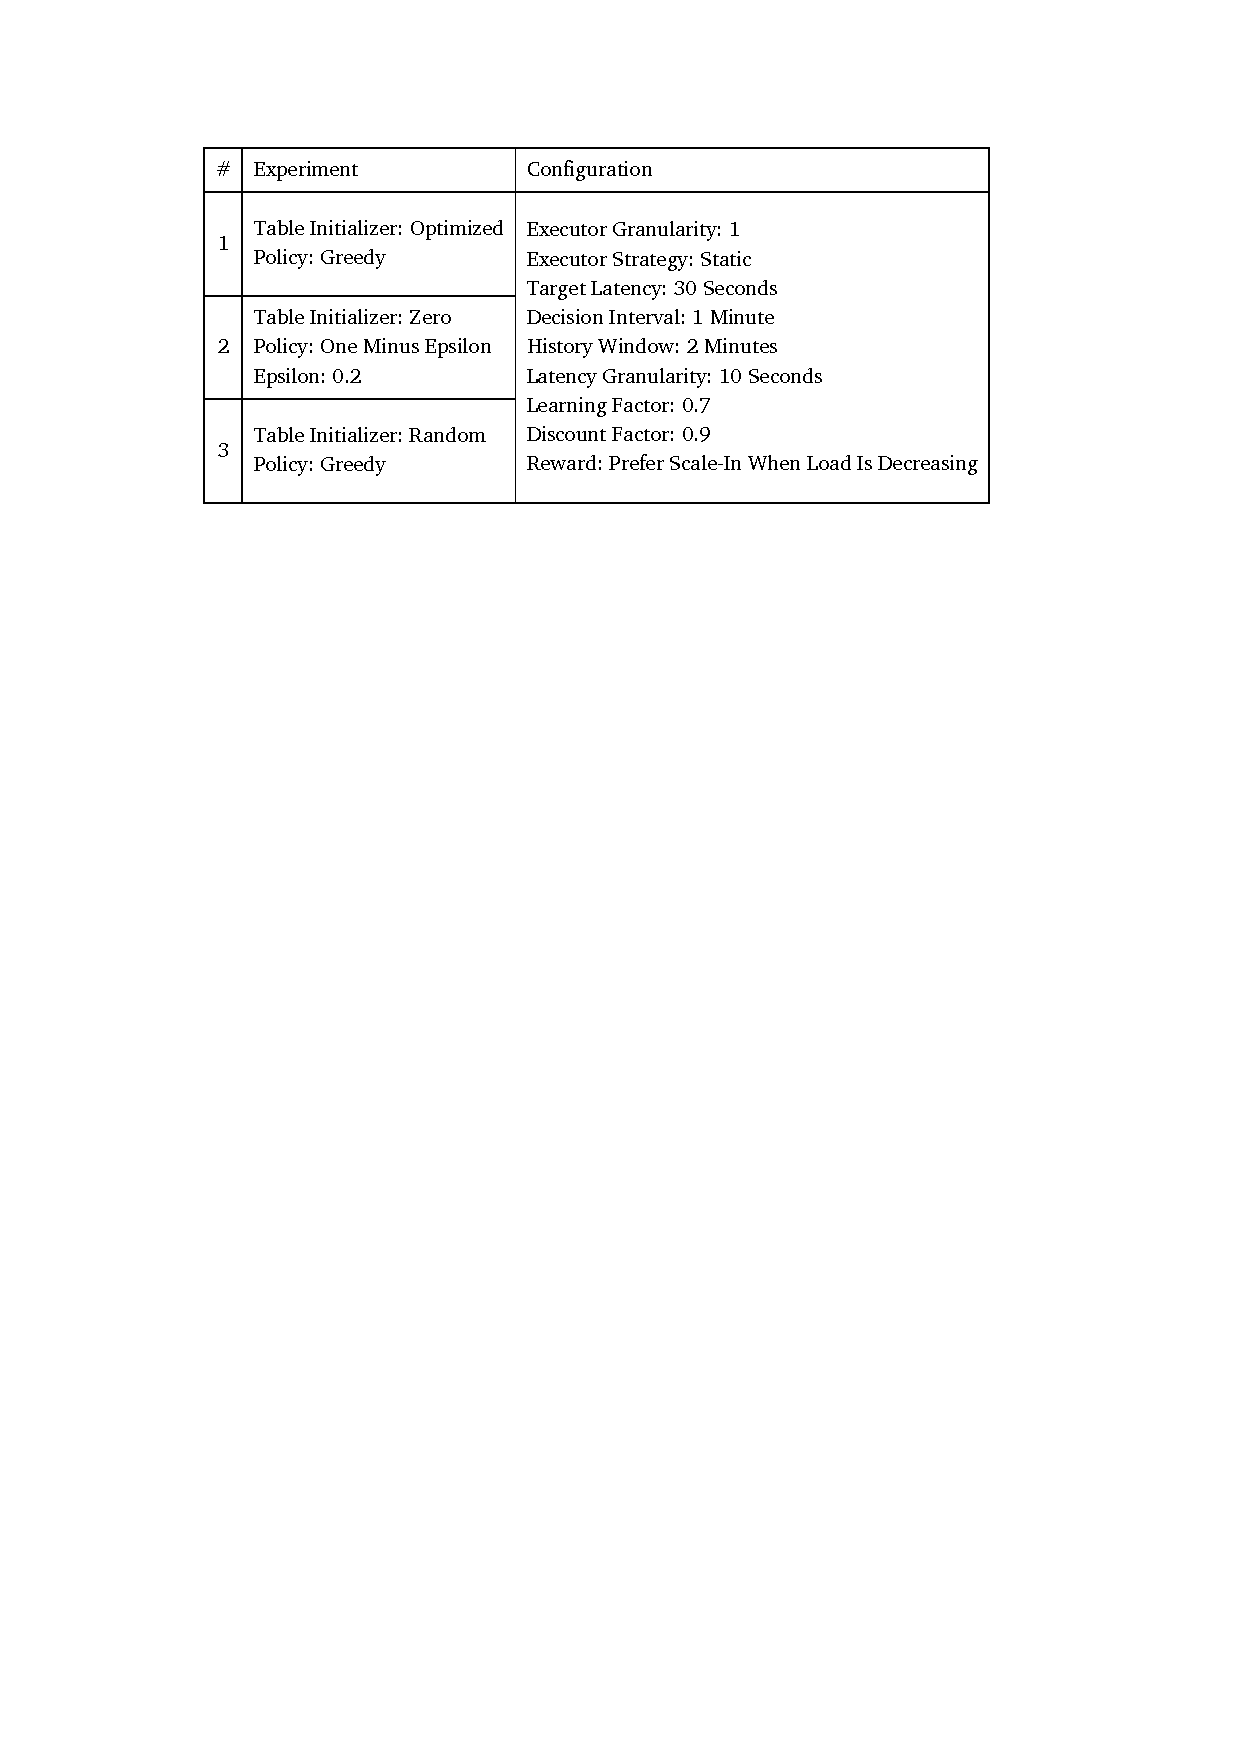
\includegraphics[clip,trim=3.3cm 21.18cm 4.1cm 2.5cm]{tables/ex4.pdf}
    \centering
    \caption{State Space Initializer Configuration Parameters}
    \label{eval:tab:ex4}
\end{table}

Figures~\ref{eval:f:e4:w1:lat},~\ref{eval:f:e4:w1:lat-c},~\ref{eval:f:e4:w1:exec} and ~\ref{eval:f:e4:w1:exec-c} illustrates latency and executor charts for Workload 1. Figures~\ref{eval:f:e4:w2:lat},~\ref{eval:f:e4:w2:lat-c},~\ref{eval:f:e4:w2:exec} and~\ref{eval:f:e4:w2:exec-c} illustrates latency and executor charts for Workload 2.

\begin{figure}[!htbp]
    \centering
    \begin{gnuplot}[terminal=epslatex, terminaloptions=color colortext]
        set terminal epslatex size 16cm,7.5cm
        set key outside center top horizontal
        set datafile separator ';'
        set xdata time
        set timefmt '%H:%M:%S'
        set xr ['0:00:00':'1:00:00']
        set yr [0:240]
        set xtics '00:00:00',600 nomirror
        set ytics 0,30 nomirror
        set y2r [0:240]
        set y2tics 0,30 nomirror
        set samples 50000 
        unset mxtics
        unset mytics
        set grid ytics lc rgb "#bbbbbb" lw 1 lt 0
        set grid xtics lc rgb "#bbbbbb" lw 1 lt 0
        unset xl
        set yl 'Latency (Seconds)'
        plot 'ex/e4/w1/latency.csv' using 1:2 w l lc 'red' lw 4 smooth csplines t 'Optimized',\
        '' using 1:3 w l lc 'blue' lw 4 smooth csplines t 'Zero',\
        '' using 1:4 w l lc 'black' lw 4 smooth csplines t 'Random'
    \end{gnuplot}
    \caption{State Space Initializer -- Workload 1 -- Latency}
    \label{eval:f:e4:w1:lat}
\end{figure}
\begin{figure}[!htbp]
    \centering
    \begin{minipage}[h]{\linewidth}
        \centering
        \begin{gnuplot}[terminal=epslatex, terminaloptions=color colortext]
            set terminal epslatex size 16cm,7.5cm
            set key outside center top horizontal
            set datafile separator ';'
            set key width -12
            set xr [0.5:3.5]
            set yr [0:240]
            set ytics 0,30 nomirror
            set y2r [0:240]
            set y2tics 0,30 nomirror
            set boxwidth 0.3 absolute
            set style fill empty
            set grid ytics lc rgb "#bbbbbb" lw 1 lt 0
            set grid xtics lc rgb "#bbbbbb" lw 1 lt 0
            unset xl
            set yl 'Latency (Seconds)'
            plot 'ex/e4/w1/latency-c.csv' using 1:2:3:4:5:xticlabels(7) with candlesticks lc 'black' lw 4 t 'Min/Max/Percentiles',\
            '' using 1:6:6:6:6 with linespoints pt 5 lc 'black' lw 4 t 'Average',\
            30 dashtype 2 lc 'black' lw 4 t 'Target'
        \end{gnuplot}
        \caption{State Space Initializer -- Workload 1 -- Latency}
        \label{eval:f:e4:w1:lat-c}
    \end{minipage}\hfil
    \begin{minipage}[h]{\linewidth}
        \centering
        \begin{gnuplot}[terminal=epslatex, terminaloptions=color colortext]
            set terminal epslatex size 16cm,7.5cm
            set key outside center top horizontal
            set datafile separator ';'
            set xdata time
            set timefmt '%H:%M:%S'
            set xr ['0:00:00':'1:00:00']
            set yr [2:26]
            set y2r [2:26]
            set ytics 0,4 nomirror
            set xtics '00:00:00',600 nomirror
            set y2tics 0,4 nomirror
            unset mxtics
            unset mytics
            set grid ytics lc rgb "#bbbbbb" lw 1 lt 0
            set grid xtics lc rgb "#bbbbbb" lw 1 lt 0
            unset xl
            set yl 'Number of Executors'
            plot 'ex/e4/w1/exec.csv' using 1:2 w l lc 'red' lw 4 t 'Optimized',\
            '' using 1:3 w l lc 'blue' lw 4 t 'Zero',\
            '' using 1:4 w l lc 'black' lw 4 t 'Random'
        \end{gnuplot}
        \caption{State Space Initializer -- Workload 1 -- Number of Executors}
        \label{eval:f:e4:w1:exec}
    \end{minipage}\hfil
    \begin{minipage}[h]{\linewidth}
        \centering
        \begin{gnuplot}[terminal=epslatex, terminaloptions=color colortext]
            set terminal epslatex size 16cm,7.5cm
            set key outside center top horizontal
            set datafile separator ';'
            set xr [0.5:3.5]
            set yr [2:26]
            set y2r [2:26]
            set ytics 0,4 nomirror
            set y2tics 0,4 nomirror
            set boxwidth 0.3 absolute
            set style fill empty
            unset xl
            set grid ytics lc rgb "#bbbbbb" lw 1 lt 0
            set grid xtics lc rgb "#bbbbbb" lw 1 lt 0
            set yl 'Number of Executors'
            plot 'ex/e4/w1/exec-c.csv' using 1:2:3:4:5:xticlabels(7) with candlesticks lc 'black' lw 4 t 'Min/Max/Percentiles',\
            '' using 1:6:6:6:6 with linespoints pt 5 lc 'black' lw 4 t 'Average' 
        \end{gnuplot}
        \caption{State Space Initializer -- Workload 1 -- Number of Executors}
        \label{eval:f:e4:w1:exec-c}
    \end{minipage}
\end{figure}
\begin{figure}[!htbp]
    \centering
    \begin{minipage}[h]{\linewidth}
        \centering
        \begin{gnuplot}[terminal=epslatex, terminaloptions=color colortext]
            set terminal epslatex size 16cm,7.5cm
            set key outside center top horizontal
            set datafile separator ';'
            set xdata time
            set timefmt '%H:%M:%S'
            set xr ['0:00:00':'1:00:00']
            set yr [0:410]
            set y2r [0:410]
            set xtics '00:00:00',600 nomirror
            set ytics 0,50 nomirror
            set y2tics 0,50 nomirror
            unset mxtics
            unset mytics
            set samples 50000 
            unset xl
            set grid ytics lc rgb "#bbbbbb" lw 1 lt 0
            set grid xtics lc rgb "#bbbbbb" lw 1 lt 0
            set yl 'Latency (Seconds)'
            plot 'ex/e4/w2/latency.csv' using 1:2 w l lc 'red' lw 4 smooth csplines t 'Optimized',\
            '' using 1:3 w l lc 'blue' lw 4 smooth csplines t 'Zero',\
            '' using 1:4 w l lc 'black' lw 4 smooth csplines t 'Random'
        \end{gnuplot}
        \caption{State Space Initializer -- Workload 2 -- Latency}
        \label{eval:f:e4:w2:lat}
    \end{minipage}\hfil
    \begin{minipage}[h]{\linewidth}
        \centering
        \begin{gnuplot}[terminal=epslatex, terminaloptions=color colortext]
            set terminal epslatex size 16cm,7.5cm
            set key outside center top horizontal
            set datafile separator ';'
            set key width -12
            set xr [0.5:3.5]
            set yr [0:410]
            set y2r [0:410]
            set ytics 0,50 nomirror
            set y2tics 0,50 nomirror
            set boxwidth 0.3 absolute
            set style fill empty
            unset xl
            set grid ytics lc rgb "#bbbbbb" lw 1 lt 0
            set grid xtics lc rgb "#bbbbbb" lw 1 lt 0            
            set yl 'Latency (Seconds)'
            plot 'ex/e4/w2/latency-c.csv' using 1:2:3:4:5:xticlabels(7) with candlesticks lc 'black' lw 4 t 'Min/Max/Percentiles',\
            '' using 1:6:6:6:6 with linespoints pt 5 lc 'black' lw 4 t 'Average',\
            30 dashtype 2 lc 'black' lw 4 t 'Target'
        \end{gnuplot}
        \caption{State Space Initializer -- Workload 2 -- Latency}
        \label{eval:f:e4:w2:lat-c}
    \end{minipage}\hfil
    \begin{minipage}[h]{\linewidth}
        \centering
        \begin{gnuplot}[terminal=epslatex, terminaloptions=color colortext]
            set terminal epslatex size 16cm,7.5cm
            set key outside center top horizontal
            set datafile separator ';'
            set xdata time
            set timefmt '%H:%M:%S'
            set xr ['0:00:00':'1:00:00']
            set yr [2:26]
            set y2r [2:26]
            set xtics '00:00:00',600 nomirror
            set ytics 0,4 nomirror
            set y2tics 0,4 nomirror
            unset mxtics
            unset mytics
            unset xl
            set grid ytics lc rgb "#bbbbbb" lw 1 lt 0
            set grid xtics lc rgb "#bbbbbb" lw 1 lt 0     
            set yl 'Number of Executors'
            plot 'ex/e4/w2/exec.csv' using 1:2 w l lc 'red' lw 4 t 'Optimized',\
            '' using 1:3 w l lc 'blue' lw 4 t 'Zero',\
            '' using 1:4 w l lc 'black' lw 4 t 'Random'
        \end{gnuplot}
        \caption{State Space Initializer -- Workload 2 -- Number of Executors}
        \label{eval:f:e4:w2:exec}
    \end{minipage}
\end{figure}
\begin{figure}[!htbp]
    \centering
    \begin{gnuplot}[terminal=epslatex, terminaloptions=color colortext]
        set terminal epslatex size 16cm,7.5cm
        set key outside center top horizontal
        set datafile separator ';'
        set xr [0.5:3.5]
        set yr [2:26]
        set ytics 0,4 nomirror
        set y2r [2:26]
        set y2tics 0,4 nomirror
        set boxwidth 0.3 absolute
        set style fill empty
        unset xl
        set grid ytics lc rgb "#bbbbbb" lw 1 lt 0
        set grid xtics lc rgb "#bbbbbb" lw 1 lt 0  
        set yl 'Number of Executors'
        plot 'ex/e4/w2/exec-c.csv' using 1:2:3:4:5:xticlabels(7) with candlesticks lc 'black' lw 4 t 'Min/Max/Percentiles','' using 1:6:6:6:6 with linespoints pt 5 lc 'black' lw 4 t 'Average' 
    \end{gnuplot}
    \caption{State Space Initializer -- Workload 2 -- Number of Executors}
    \label{eval:f:e4:w2:exec-c}
\end{figure}
\FloatBarrier
\subsection{Conclusion}

For Workload 1 as depicted, optimized initializer beats zero and random initializers and to a large degree it is able to respect target latency. For Workload 2, random initializer performs similar to optimized initializer. But this is only achieved by chance. Looking at Figure~\ref{eval:f:e4:w2:exec} reveals two pieces of information.
\begin{itemize}
    \item Since the first part of Workload 2 is not intensive and Auto-Scaler is running with minimum executors, random initializer performs early Scale-Out -- there is no other option with minimum executors. Since this action helps to improve the latency, Auto-Scaler learns this bit of information and performs another Scale-Out which in turn improves latency further. Up until the workload reaches critical point -- in terms of latency -- Auto-Scaler has already performed consecutive Scale-Out actions which helps to diverge faster. Note that if the workload begins with a peak -- just like Workload 1, there is little chance that random initializer could win the game.
    \item Considering final stage of workload, where Auto-Scaler has removed so many executors that the latency started to increase fast -- Figure~\ref{eval:f:e4:w2:lat} -- which indicates state space still contains wrong information. Note that optimized initializer removes executors at a slower rate.
\end{itemize}

Looking at behavior of zero initializer reveals an interesting point. Since Auto-Scaler has started with minimum executors, it wasn't able to process the workload. On the other hand all states are initialized to zero. Thus, Auto-Scaler will stick to No-Action -- with a probability of $\epsilon$ will perform random action. Staying with No-Action leads to even higher latency which is a new state initialized with zero. Again, Auto-Scaler will stick to No-Action which in turn increases latency and causes Auto-Scaler to land in another new state. This process keeps going -- latency increases leading Auto-Scaler to land in a new state. This means, Auto-Scaler never sees the previous states to utilize learned information. This is the point where Queue-Aware executor strategy could potentially help to complement Auto-Scaler's actions. In case Auto-Scaler is behind schedule and by any chance takes a random Scale-Out action, Queue-Aware strategy adds a batch of executors at once which would considerably improve latency.

In general, if an Auto-Scaler starts with zero or random initializer, it is better to start with maximum -- or at least reasonable -- number of executors such that initial random actions don't cause serious SLO violations.

\clearpage
\section{Experiment 5: Learning Factor}
As mentioned in previous chapters, A Q-Learning agent learns new information and merges it with its own knowledge. The speed of learning is controlled by learning factor which defined by \lstinline|learningFactor| in this thesis. This experiment has been designed to show the effect of different learning factor values. Note that learning factor affects Auto-Scaler's behavior in long run. Thus, for a 1-Hour experiment extreme values should be chosen to make difference observable. Furthermore, since there is no random action involved in this experiment, Queue Aware executor strategy can be used again. Table~\ref{eval:tab:ex5} describes the configuration parameters of this experiment. 
\begin{table}[h]
    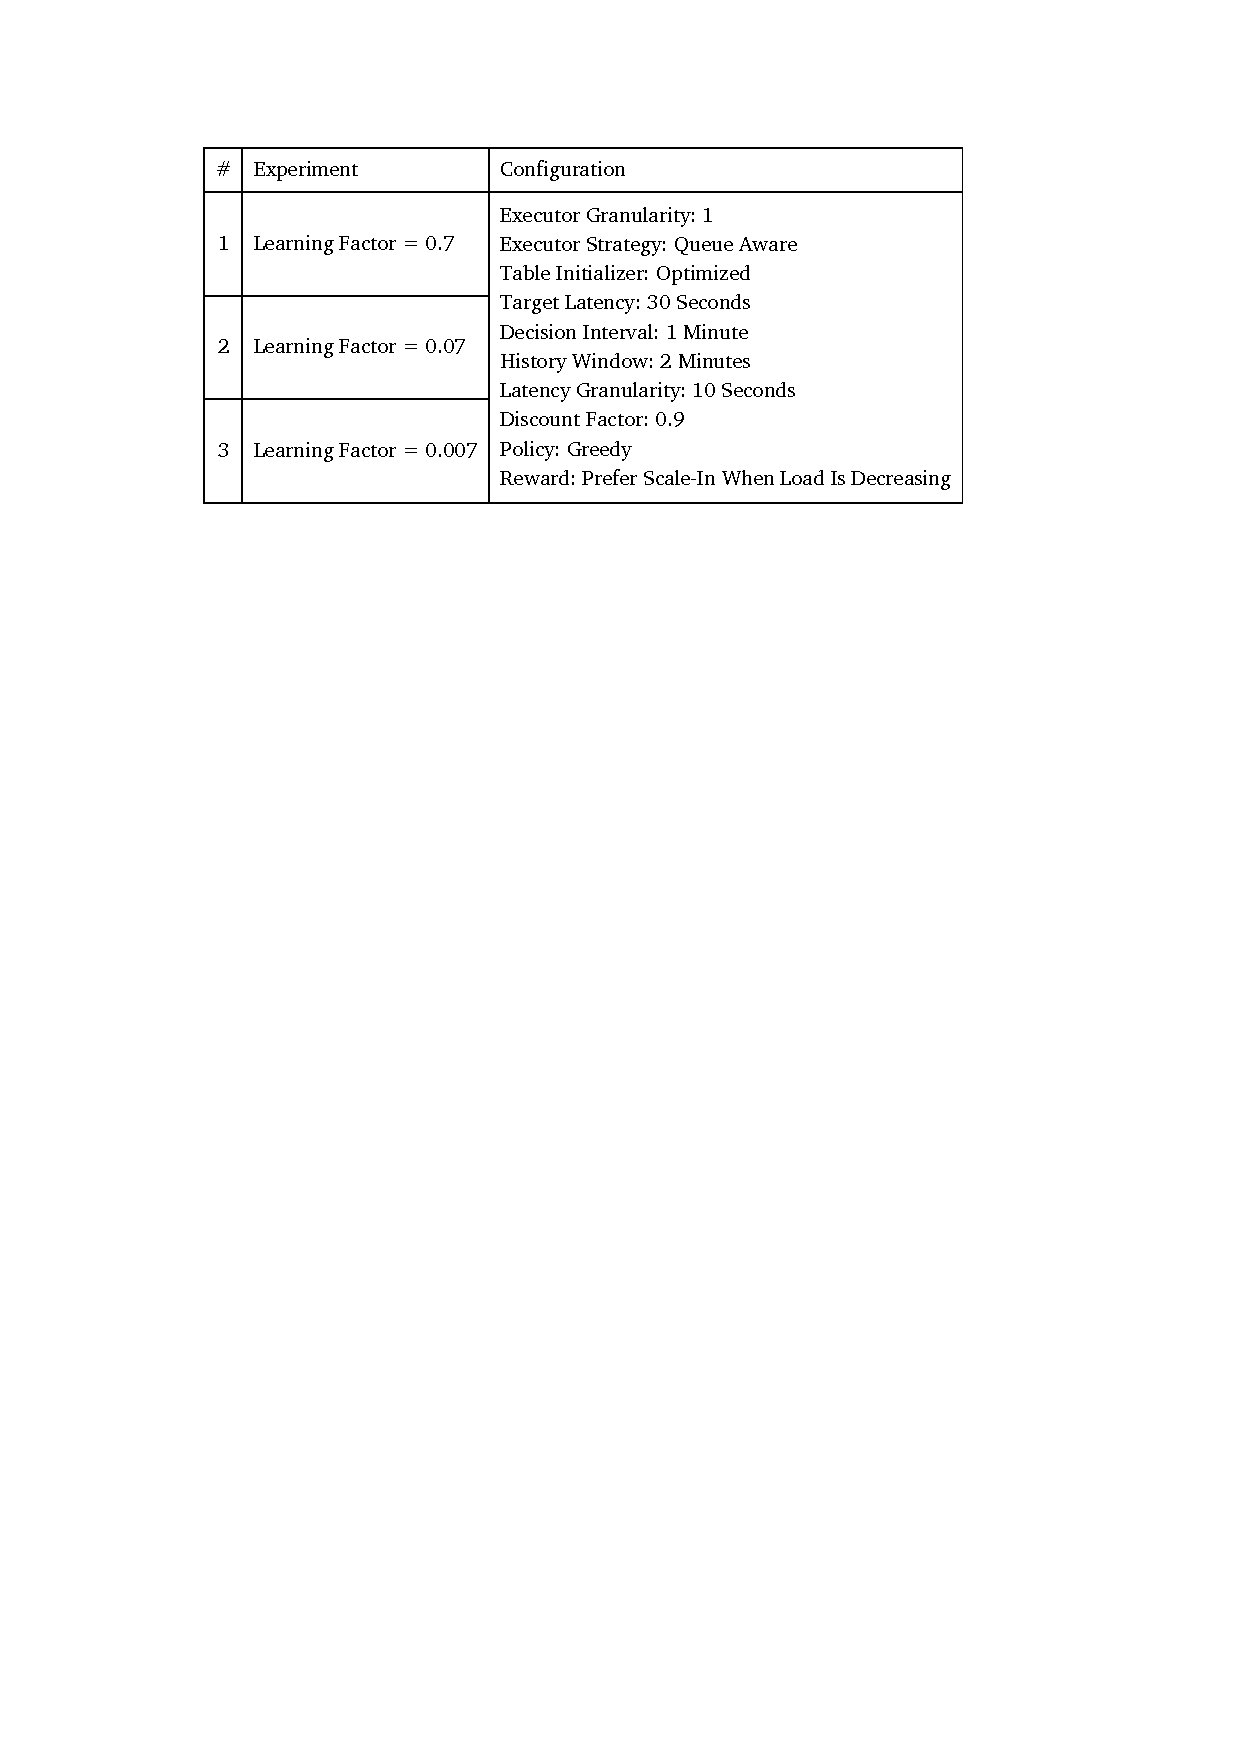
\includegraphics[clip,trim=3.3cm 21.18cm 4.5cm 2.5cm]{tables/ex5.pdf}
    \centering
    \caption{Learning Factor Configuration Parameters}
    \label{eval:tab:ex5}
\end{table}

Figures~\ref{eval:f:e5:w1:lat},~\ref{eval:f:e5:w1:lat-c},~\ref{eval:f:e5:w1:exec} and ~\ref{eval:f:e5:w1:exec-c} illustrates latency and executor charts for Workload 1. Figures~\ref{eval:f:e5:w2:lat},~\ref{eval:f:e5:w2:lat-c},~\ref{eval:f:e5:w2:exec} and~\ref{eval:f:e5:w2:exec-c} illustrates latency and executor charts for Workload 2.

\begin{figure}[!htbp]
    \centering
    \begin{gnuplot}[terminal=epslatex, terminaloptions=color colortext]
        set terminal epslatex size 16cm,7.5cm
        set key outside center top horizontal
        set datafile separator ';'
        set xdata time
        set timefmt '%H:%M:%S'
        set xr ['0:00:00':'1:00:00']
        set yr [0:150]
        set xtics '00:00:00',600 nomirror
        set ytics 0,30 nomirror
        set y2r [0:150]
        set y2tics 0,30 nomirror
        set samples 50000 
        unset mxtics
        unset mytics
        set grid ytics lc rgb "#bbbbbb" lw 1 lt 0
        set grid xtics lc rgb "#bbbbbb" lw 1 lt 0
        unset xl
        set yl 'Latency (Seconds)'
        plot 'ex/e5/w1/latency.csv' using 1:2 w l lc 'red' lw 4 smooth csplines t '0.7',\
        '' using 1:3 w l lc 'blue' lw 4 smooth csplines t '0.07',\
        '' using 1:4 w l lc 'black' lw 4 smooth csplines t '0.007'
    \end{gnuplot}
    \caption{Learning Factor -- Workload 1 -- Latency}
    \label{eval:f:e5:w1:lat}
\end{figure}
\begin{figure}[!htbp]
    \centering
    \begin{minipage}[h]{\linewidth}
        \centering
        \begin{gnuplot}[terminal=epslatex, terminaloptions=color colortext]
            set terminal epslatex size 16cm,7.5cm
            set key outside center top horizontal
            set datafile separator ';'
            set key width -12
            set xr [0.5:3.5]
            set yr [0:150]
            set ytics 0,30 nomirror
            set y2r [0:150]
            set y2tics 0,30 nomirror
            set boxwidth 0.3 absolute
            set style fill empty
            set grid ytics lc rgb "#bbbbbb" lw 1 lt 0
            set grid xtics lc rgb "#bbbbbb" lw 1 lt 0
            unset xl
            set yl 'Latency (Seconds)'
            plot 'ex/e5/w1/latency-c.csv' using 1:2:3:4:5:xticlabels(7) with candlesticks lc 'black' lw 4 t 'Min/Max/Percentiles',\
            '' using 1:6:6:6:6 with linespoints pt 5 lc 'black' lw 4 t 'Average',\
            30 dashtype 2 lc 'black' lw 4 t 'Target'
        \end{gnuplot}
        \caption{Learning Factor -- Workload 1 -- Latency}
        \label{eval:f:e5:w1:lat-c}
    \end{minipage}\hfil
    \begin{minipage}[h]{\linewidth}
        \centering
        \begin{gnuplot}[terminal=epslatex, terminaloptions=color colortext]
            set terminal epslatex size 16cm,7.5cm
            set key outside center top horizontal
            set datafile separator ';'
            set xdata time
            set timefmt '%H:%M:%S'
            set xr ['0:00:00':'1:00:00']
            set yr [2:26]
            set y2r [2:26]
            set ytics 0,4 nomirror
            set xtics '00:00:00',600 nomirror
            set y2tics 0,4 nomirror
            unset mxtics
            unset mytics
            set grid ytics lc rgb "#bbbbbb" lw 1 lt 0
            set grid xtics lc rgb "#bbbbbb" lw 1 lt 0
            unset xl
            set yl 'Number of Executors'
            plot 'ex/e5/w1/exec.csv' using 1:2 w l lc 'red' lw 4 t '0.7',\
            '' using 1:3 w l lc 'blue' lw 4 t '0.07',\
            '' using 1:4 w l lc 'black' lw 4 t '0.007'
        \end{gnuplot}
        \caption{Learning Factor -- Workload 1 -- Number of Executors}
        \label{eval:f:e5:w1:exec}
    \end{minipage}\hfil
    \begin{minipage}[h]{\linewidth}
        \centering
        \begin{gnuplot}[terminal=epslatex, terminaloptions=color colortext]
            set terminal epslatex size 16cm,7.5cm
            set key outside center top horizontal
            set datafile separator ';'
            set xr [0.5:3.5]
            set yr [2:26]
            set y2r [2:26]
            set ytics 0,4 nomirror
            set y2tics 0,4 nomirror
            set boxwidth 0.3 absolute
            set style fill empty
            unset xl
            set grid ytics lc rgb "#bbbbbb" lw 1 lt 0
            set grid xtics lc rgb "#bbbbbb" lw 1 lt 0
            set yl 'Number of Executors'
            plot 'ex/e5/w1/exec-c.csv' using 1:2:3:4:5:xticlabels(7) with candlesticks lc 'black' lw 4 t 'Min/Max/Percentiles',\
            '' using 1:6:6:6:6 with linespoints pt 5 lc 'black' lw 4 t 'Average' 
        \end{gnuplot}
        \caption{Learning Factor -- Workload 1 -- Number of Executors}
        \label{eval:f:e5:w1:exec-c}
    \end{minipage}
\end{figure}
\begin{figure}[!htbp]
    \centering
    \begin{minipage}[h]{\linewidth}
        \centering
        \begin{gnuplot}[terminal=epslatex, terminaloptions=color colortext]
            set terminal epslatex size 16cm,7.5cm
            set key outside center top horizontal
            set datafile separator ';'
            set xdata time
            set timefmt '%H:%M:%S'
            set xr ['0:00:00':'1:00:00']
            set yr [0:120]
            set y2r [0:120]
            set xtics '00:00:00',600 nomirror
            set ytics 0,30 nomirror
            set y2tics 0,30 nomirror
            unset mxtics
            unset mytics
            set samples 50000 
            unset xl
            set grid ytics lc rgb "#bbbbbb" lw 1 lt 0
            set grid xtics lc rgb "#bbbbbb" lw 1 lt 0
            set yl 'Latency (Seconds)'
            plot 'ex/e5/w2/latency.csv' using 1:2 w l lc 'red' lw 4 smooth csplines t '0.7',\
            '' using 1:3 w l lc 'blue' lw 4 smooth csplines t '0.07',\
            '' using 1:4 w l lc 'black' lw 4 smooth csplines t '0.007'
        \end{gnuplot}
        \caption{Learning Factor -- Workload 2 -- Latency}
        \label{eval:f:e5:w2:lat}
    \end{minipage}\hfil
    \begin{minipage}[h]{\linewidth}
        \centering
        \begin{gnuplot}[terminal=epslatex, terminaloptions=color colortext]
            set terminal epslatex size 16cm,7.5cm
            set key outside center top horizontal
            set datafile separator ';'
            set key width -12
            set xr [0.5:3.5]
            set yr [0:120]
            set y2r [0:120]
            set ytics nomirror
            set y2tics 0,30 nomirror
            set ytics 0,30 nomirror
            set boxwidth 0.3 absolute
            set style fill empty
            unset xl
            set grid ytics lc rgb "#bbbbbb" lw 1 lt 0
            set grid xtics lc rgb "#bbbbbb" lw 1 lt 0            
            set yl 'Latency (Seconds)'
            plot 'ex/e5/w2/latency-c.csv' using 1:2:3:4:5:xticlabels(7) with candlesticks lc 'black' lw 4 t 'Min/Max/Percentiles',\
            '' using 1:6:6:6:6 with linespoints pt 5 lc 'black' lw 4 t 'Average',\
            30 dashtype 2 lc 'black' lw 4 t 'Target'
        \end{gnuplot}
        \caption{Learning Factor -- Workload 2 -- Latency}
        \label{eval:f:e5:w2:lat-c}
    \end{minipage}\hfil
    \begin{minipage}[h]{\linewidth}
        \centering
        \begin{gnuplot}[terminal=epslatex, terminaloptions=color colortext]
            set terminal epslatex size 16cm,7.5cm
            set key outside center top horizontal
            set datafile separator ';'
            set xdata time
            set timefmt '%H:%M:%S'
            set xr ['0:00:00':'1:00:00']
            set yr [2:26]
            set y2r [2:26]
            set xtics '00:00:00',600 nomirror
            set ytics 0,4 nomirror
            set y2tics 0,4 nomirror
            unset mxtics
            unset mytics
            unset xl
            set grid ytics lc rgb "#bbbbbb" lw 1 lt 0
            set grid xtics lc rgb "#bbbbbb" lw 1 lt 0     
            set yl 'Number of Executors'
            plot 'ex/e5/w2/exec.csv' using 1:2 w l lc 'red' lw 4 t '0.7',\
            '' using 1:3 w l lc 'blue' lw 4 t '0.07',\
            '' using 1:4 w l lc 'black' lw 4 t '0.007'
        \end{gnuplot}
        \caption{Learning Factor -- Workload 2 -- Number of Executors}
        \label{eval:f:e5:w2:exec}
    \end{minipage}
\end{figure}
\begin{figure}[!htbp]
    \centering
    \begin{gnuplot}[terminal=epslatex, terminaloptions=color colortext]
        set terminal epslatex size 16cm,7.5cm
        set key outside center top horizontal
        set datafile separator ';'
        set xr [0.5:3.5]
        set yr [2:26]
        set ytics 0,4 nomirror
        set y2r [2:26]
        set y2tics 0,4 nomirror
        set boxwidth 0.3 absolute
        set style fill empty
        unset xl
        set grid ytics lc rgb "#bbbbbb" lw 1 lt 0
        set grid xtics lc rgb "#bbbbbb" lw 1 lt 0  
        set yl 'Number of Executors'
        plot 'ex/e5/w2/exec-c.csv' using 1:2:3:4:5:xticlabels(7) with candlesticks lc 'black' lw 4 t 'Min/Max/Percentiles','' using 1:6:6:6:6 with linespoints pt 5 lc 'black' lw 4 t 'Average' 
    \end{gnuplot}
    \caption{Learning Factor -- Workload 2 -- Number of Executors}
    \label{eval:f:e5:w2:exec-c}
\end{figure}
\FloatBarrier
\subsection{Conclusion}
For Workload 1, learning factor of 0.7 achieves a better result both in terms of latency and number of executors. It is tempting to conclude that for unpredictable workloads, it is better to apply a higher learning factor.

But the above conclusion doesn't hold when we look at the result of Workload 2. In terms of latency, 0.007 is slightly below target latency which is better than 0.7 and 0.07. In terms of number of executors, it achieves an outstanding result of 8 executors on average. Combining latency and number of executors this is the best result that has been achieved for Workload 2.

It seems that the effect of learning factor is totally workload dependent and no generalized conclusion can be made based on these two workloads.
\clearpage
\section{Experiment 6: Discretization}
This experiment has been designed to evaluate the effect of discretization on Auto-Scaler's decisions. Discretization is applied to both latency and incoming messages. Table~\ref{eval:tab:ex6} describes the configuration parameters of this experiment.
\begin{table}[h]
    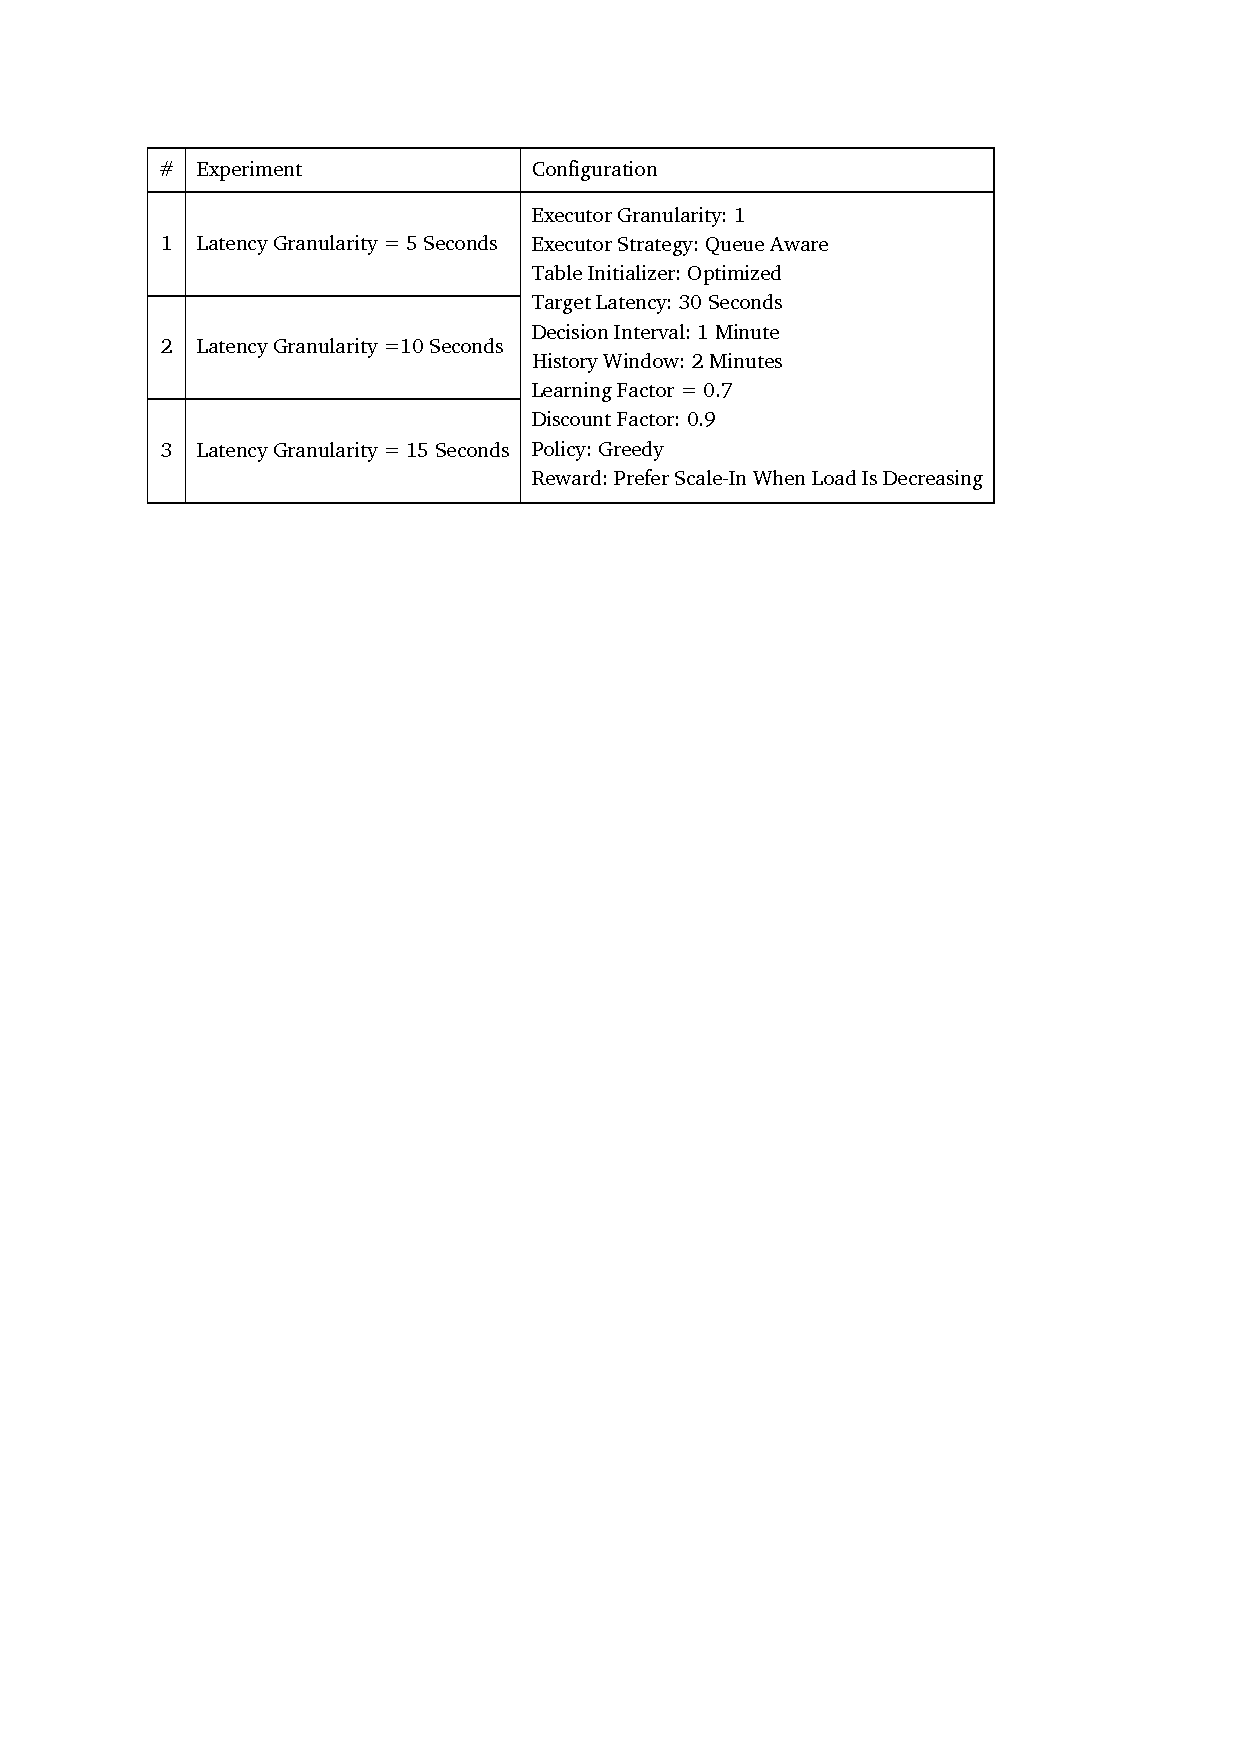
\includegraphics[clip,trim=2.2cm 21.18cm 3cm 2.5cm]{tables/ex6.pdf}
    \centering
    \caption{Discretization Configuration Parameters}
    \label{eval:tab:ex6}
\end{table}

Figures~\ref{eval:f:e6:w1:lat},~\ref{eval:f:e6:w1:lat-c},~\ref{eval:f:e6:w1:exec} and ~\ref{eval:f:e6:w1:exec-c} illustrates latency and executor charts for Workload 1. Figures~\ref{eval:f:e6:w2:lat},~\ref{eval:f:e6:w2:lat-c},~\ref{eval:f:e6:w2:exec} and~\ref{eval:f:e6:w2:exec-c} illustrates latency and executor charts for Workload 2.

\begin{figure}[!htbp]
    \centering
    \begin{gnuplot}[terminal=epslatex, terminaloptions=color colortext]
        set terminal epslatex size 16cm,7.5cm
        set key outside center top horizontal
        set datafile separator ';'
        set xdata time
        set timefmt '%H:%M:%S'
        set xr ['0:00:00':'1:00:00']
        set yr [0:120]
        set xtics '00:00:00',600 nomirror
        set ytics 0,30 nomirror
        set y2r [0:120]
        set y2tics 0,30 nomirror
        set samples 50000 
        unset mxtics
        unset mytics
        set grid ytics lc rgb "#bbbbbb" lw 1 lt 0
        set grid xtics lc rgb "#bbbbbb" lw 1 lt 0
        unset xl
        set yl 'Latency (Seconds)'
        plot 'ex/e6/w1/latency.csv' using 1:2 w l lc 'red' lw 4 smooth csplines t '5 Sec',\
        '' using 1:3 w l lc 'blue' lw 4 smooth csplines t '10 Sec',\
        '' using 1:4 w l lc 'black' lw 4 smooth csplines t '15 Sec'
    \end{gnuplot}
    \caption{Discretization -- Workload 1 -- Latency}
    \label{eval:f:e6:w1:lat}
\end{figure}
\begin{figure}[!htbp]
    \centering
    \begin{minipage}[h]{\linewidth}
        \centering
        \begin{gnuplot}[terminal=epslatex, terminaloptions=color colortext]
            set terminal epslatex size 16cm,7.5cm
            set key outside center top horizontal
            set datafile separator ';'
            set key width -12
            set xr [0.5:3.5]
            set yr [0:120]
            set ytics 0,30 nomirror
            set y2r [0:120]
            set y2tics 0,30 nomirror
            set boxwidth 0.3 absolute
            set style fill empty
            set grid ytics lc rgb "#bbbbbb" lw 1 lt 0
            set grid xtics lc rgb "#bbbbbb" lw 1 lt 0
            unset xl
            set yl 'Latency (Seconds)'
            plot 'ex/e6/w1/latency-c.csv' using 1:2:3:4:5:xticlabels(7) with candlesticks lc 'black' lw 4 t 'Min/Max/Percentiles',\
            '' using 1:6:6:6:6 with linespoints pt 5 lc 'black' lw 4 t 'Average',\
            30 dashtype 2 lc 'black' lw 4 t 'Target'
        \end{gnuplot}
        \caption{Discretization -- Workload 1 -- Latency}
        \label{eval:f:e6:w1:lat-c}
    \end{minipage}\hfil
    \begin{minipage}[h]{\linewidth}
        \centering
        \begin{gnuplot}[terminal=epslatex, terminaloptions=color colortext]
            set terminal epslatex size 16cm,7.5cm
            set key outside center top horizontal
            set datafile separator ';'
            set xdata time
            set timefmt '%H:%M:%S'
            set xr ['0:00:00':'1:00:00']
            set yr [2:26]
            set y2r [2:26]
            set ytics 0,4 nomirror
            set xtics '00:00:00',600 nomirror
            set y2tics 0,4 nomirror
            unset mxtics
            unset mytics
            set grid ytics lc rgb "#bbbbbb" lw 1 lt 0
            set grid xtics lc rgb "#bbbbbb" lw 1 lt 0
            unset xl
            set yl 'Number of Executors'
            plot 'ex/e6/w1/exec.csv' using 1:2 w l lc 'red' lw 4 t '5 Sec',\
            '' using 1:3 w l lc 'blue' lw 4 t '10 Sec',\
            '' using 1:4 w l lc 'black' lw 4 t '15 Sec'
        \end{gnuplot}
        \caption{Discretization -- Workload 1 -- Number of Executors}
        \label{eval:f:e6:w1:exec}
    \end{minipage}\hfil
    \begin{minipage}[h]{\linewidth}
        \centering
        \begin{gnuplot}[terminal=epslatex, terminaloptions=color colortext]
            set terminal epslatex size 16cm,7.5cm
            set key outside center top horizontal
            set datafile separator ';'
            set xr [0.5:3.5]
            set yr [2:26]
            set y2r [2:26]
            set ytics 0,4 nomirror
            set y2tics 0,4 nomirror
            set boxwidth 0.3 absolute
            set style fill empty
            unset xl
            set grid ytics lc rgb "#bbbbbb" lw 1 lt 0
            set grid xtics lc rgb "#bbbbbb" lw 1 lt 0
            set yl 'Number of Executors'
            plot 'ex/e6/w1/exec-c.csv' using 1:2:3:4:5:xticlabels(7) with candlesticks lc 'black' lw 4 t 'Min/Max/Percentiles',\
            '' using 1:6:6:6:6 with linespoints pt 5 lc 'black' lw 4 t 'Average' 
        \end{gnuplot}
        \caption{Discretization -- Workload 1 -- Number of Executors}
        \label{eval:f:e6:w1:exec-c}
    \end{minipage}
\end{figure}
\begin{figure}[!htbp]
    \centering
    \begin{minipage}[h]{\linewidth}
        \centering
        \begin{gnuplot}[terminal=epslatex, terminaloptions=color colortext]
            set terminal epslatex size 16cm,7.5cm
            set key outside center top horizontal
            set datafile separator ';'
            set xdata time
            set timefmt '%H:%M:%S'
            set xr ['0:00:00':'1:00:00']
            set yr [0:120]
            set y2r [0:120]
            set xtics '00:00:00',600 nomirror
            set ytics 0,30 nomirror
            set y2tics 0,30 nomirror
            unset mxtics
            unset mytics
            set samples 50000 
            unset xl
            set grid ytics lc rgb "#bbbbbb" lw 1 lt 0
            set grid xtics lc rgb "#bbbbbb" lw 1 lt 0
            set yl 'Latency (Seconds)'
            plot 'ex/e6/w2/latency.csv' using 1:2 w l lc 'red' lw 4 smooth csplines t '5 Sec',\
            '' using 1:3 w l lc 'blue' lw 4 smooth csplines t '10 Sec',\
            '' using 1:4 w l lc 'black' lw 4 smooth csplines t '15 Sec'
        \end{gnuplot}
        \caption{Discretization -- Workload 2 -- Latency}
        \label{eval:f:e6:w2:lat}
    \end{minipage}\hfil
    \begin{minipage}[h]{\linewidth}
        \centering
        \begin{gnuplot}[terminal=epslatex, terminaloptions=color colortext]
            set terminal epslatex size 16cm,7.5cm
            set key outside center top horizontal
            set datafile separator ';'
            set key width -12
            set xr [0.5:3.5]
            set yr [0:120]
            set y2r [0:120]
            set ytics 0,30 nomirror
            set y2tics 0,30 nomirror
            set boxwidth 0.3 absolute
            set style fill empty
            unset xl
            set grid ytics lc rgb "#bbbbbb" lw 1 lt 0
            set grid xtics lc rgb "#bbbbbb" lw 1 lt 0            
            set yl 'Latency (Seconds)'
            plot 'ex/e6/w2/latency-c.csv' using 1:2:3:4:5:xticlabels(7) with candlesticks lc 'black' lw 4 t 'Min/Max/Percentiles',\
            '' using 1:6:6:6:6 with linespoints pt 5 lc 'black' lw 4 t 'Average',\
            30 dashtype 2 lc 'black' lw 4 t 'Target'
        \end{gnuplot}
        \caption{Discretization -- Workload 2 -- Latency}
        \label{eval:f:e6:w2:lat-c}
    \end{minipage}\hfil
    \begin{minipage}[h]{\linewidth}
        \centering
        \begin{gnuplot}[terminal=epslatex, terminaloptions=color colortext]
            set terminal epslatex size 16cm,7.5cm
            set key outside center top horizontal
            set datafile separator ';'
            set xdata time
            set timefmt '%H:%M:%S'
            set xr ['0:00:00':'1:00:00']
            set yr [2:26]
            set y2r [2:26]
            set xtics '00:00:00',600 nomirror
            set ytics 0,4 nomirror
            set y2tics 0,4 nomirror
            unset mxtics
            unset mytics
            unset xl
            set grid ytics lc rgb "#bbbbbb" lw 1 lt 0
            set grid xtics lc rgb "#bbbbbb" lw 1 lt 0     
            set yl 'Number of Executors'
            plot 'ex/e6/w2/exec.csv' using 1:2 w l lc 'red' lw 4 t '5 Sec',\
            '' using 1:3 w l lc 'blue' lw 4 t '10 Sec',\
            '' using 1:4 w l lc 'black' lw 4 t '15 Sec'
        \end{gnuplot}
        \caption{Discretization -- Workload 2 -- Number of Executors}
        \label{eval:f:e6:w2:exec}
    \end{minipage}
\end{figure}
\begin{figure}[!htbp]
    \centering
    \begin{gnuplot}[terminal=epslatex, terminaloptions=color colortext]
        set terminal epslatex size 16cm,7.5cm
        set key outside center top horizontal
        set datafile separator ';'
        set xr [0.5:3.5]
        set yr [2:26]
        set ytics 0,4 nomirror
        set y2r [2:26]
        set y2tics 0,4 nomirror
        set boxwidth 0.3 absolute
        set style fill empty
        unset xl
        set grid ytics lc rgb "#bbbbbb" lw 1 lt 0
        set grid xtics lc rgb "#bbbbbb" lw 1 lt 0  
        set yl 'Number of Executors'
        plot 'ex/e6/w2/exec-c.csv' using 1:2:3:4:5:xticlabels(7) with candlesticks lc 'black' lw 4 t 'Min/Max/Percentiles','' using 1:6:6:6:6 with linespoints pt 5 lc 'black' lw 4 t 'Average' 
    \end{gnuplot}
    \caption{Discretization -- Workload 2 -- Number of Executors}
    \label{eval:f:e6:w2:exec-c}
\end{figure}
\FloatBarrier
\subsection{Conclusion}
For Workload 1, 5-second discretization performs better in terms of latency albeit with more executors. For Workload 2, 10-second discretization performs better both in terms of latency and number of executors.

Although 10-second discretization performs reasonably well in both workloads, we are still not sure that it is the optimal discretization. Similar to learning factor, discretization seems to be workload dependent and no generalized conclusion can be made.

\clearpage
\section{Experiment 7: Value Iteration}
\textcite{dutreilh:hal-01122123} claimed that Value Iteration algorithm helps to initialize the state table and speedup learning process. Authors conducted an experiment which was based on a sinusoidal workload. Agent is trained in first period of rotation and then standard Q-Learning is used for next rounds. However, training based on sinusoidal workload is not so challenging. In this experiment the agent is trained using a different data set than the actual workload. State space is initialized after 5, 10 and 20 minutes of training period and then Auto-Scaler's behavior is evaluated under both workloads. During training \lstinline|decreasingOneMinusEpsilon| policy is used to help agent discover the environment. However, during the evaluation greedy policy is used. Table~\ref{eval:tab:ex7} describes the configuration parameters of this experiment.
\begin{table}[h]
    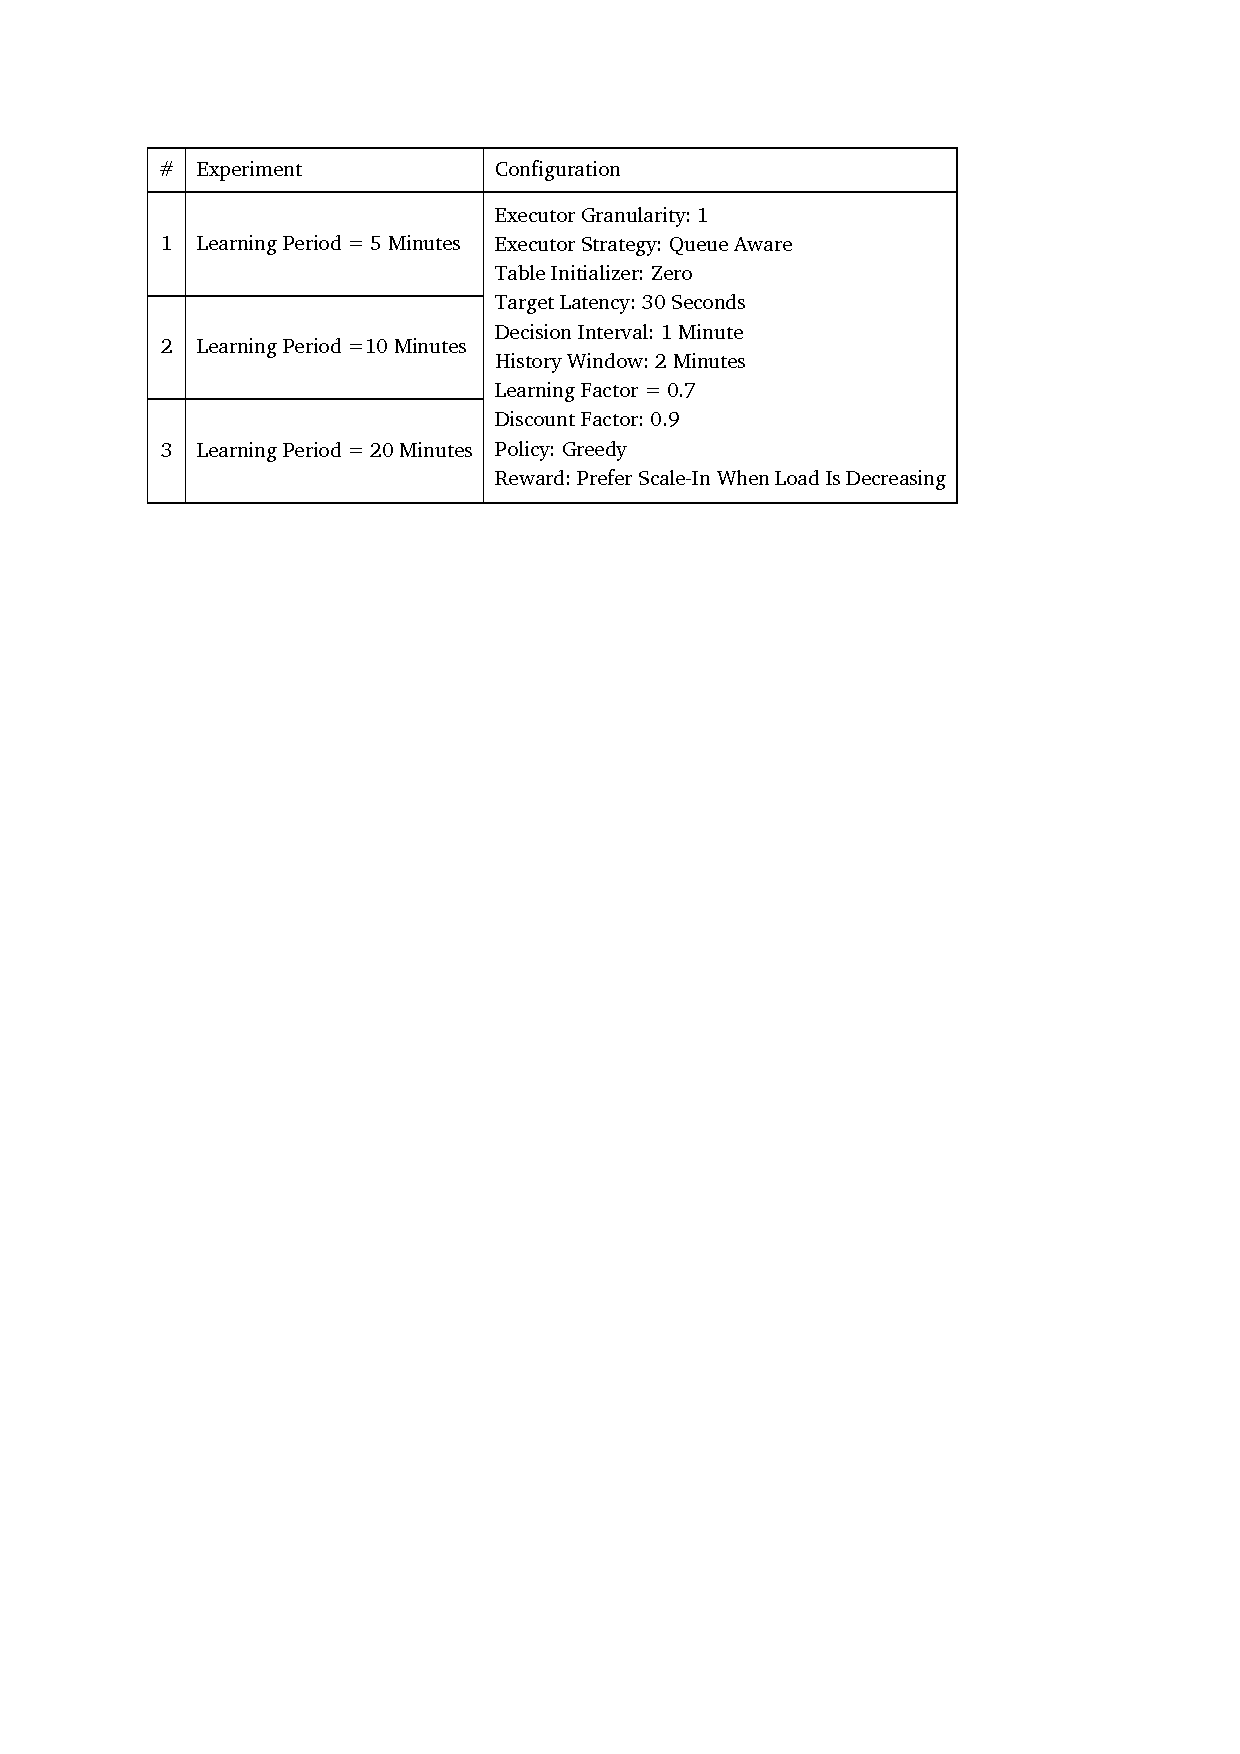
\includegraphics[clip,trim=2.4cm 21.18cm 4.65cm 2.5cm]{tables/ex7.pdf}
    \centering
    \caption{Value Iteration Configuration Parameters}
    \label{eval:tab:ex7}
\end{table}

Figures~\ref{eval:f:e7:w1:lat},~\ref{eval:f:e7:w1:lat-c},~\ref{eval:f:e7:w1:exec} and ~\ref{eval:f:e7:w1:exec-c} illustrates latency and executor charts for Workload 1. Figures~\ref{eval:f:e7:w2:lat},~\ref{eval:f:e7:w2:lat-c},~\ref{eval:f:e7:w2:exec} and~\ref{eval:f:e7:w2:exec-c} illustrates latency and executor charts for Workload 2.

\begin{figure}[!htbp]
    \centering
    \begin{gnuplot}[terminal=epslatex, terminaloptions=color colortext]
        set terminal epslatex size 16cm,7.5cm
        set key outside center top horizontal
        set datafile separator ';'
        set xdata time
        set timefmt '%H:%M:%S'
        set xr ['0:00:00':'1:00:00']
        set yr [0:210]
        set xtics '00:00:00',600 nomirror
        set ytics 0,30 nomirror
        set y2r [0:210]
        set y2tics 0,30 nomirror
        set samples 50000 
        unset mxtics
        unset mytics
        set grid ytics lc rgb "#bbbbbb" lw 1 lt 0
        set grid xtics lc rgb "#bbbbbb" lw 1 lt 0
        unset xl
        set yl 'Latency (Seconds)'
        plot 'ex/e7/w1/latency.csv' using 1:2 w l lc 'red' lw 4 smooth csplines t '5 Min',\
        '' using 1:3 w l lc 'blue' lw 4 smooth csplines t '10 Min',\
        '' using 1:4 w l lc 'black' lw 4 smooth csplines t '20 Min'
    \end{gnuplot}
    \caption{Value Iteration -- Workload 1 -- Latency}
    \label{eval:f:e7:w1:lat}
\end{figure}
\begin{figure}[!htbp]
    \centering
    \begin{minipage}[h]{\linewidth}
        \centering
        \begin{gnuplot}[terminal=epslatex, terminaloptions=color colortext]
            set terminal epslatex size 16cm,7.5cm
            set key outside center top horizontal
            set datafile separator ';'
            set key width -12
            set xr [0.5:3.5]
            set yr [0:210]
            set ytics 0,30 nomirror
            set y2r [0:210]
            set y2tics 0,30 nomirror
            set boxwidth 0.3 absolute
            set style fill empty
            set grid ytics lc rgb "#bbbbbb" lw 1 lt 0
            set grid xtics lc rgb "#bbbbbb" lw 1 lt 0
            unset xl
            set yl 'Latency (Seconds)'
            plot 'ex/e7/w1/latency-c.csv' using 1:2:3:4:5:xticlabels(7) with candlesticks lc 'black' lw 4 t 'Min/Max/Percentiles',\
            '' using 1:6:6:6:6 with linespoints pt 5 lc 'black' lw 4 t 'Average',\
            30 dashtype 2 lc 'black' lw 4 t 'Target'
        \end{gnuplot}
        \caption{Value Iteration -- Workload 1 -- Latency}
        \label{eval:f:e7:w1:lat-c}
    \end{minipage}\hfil
    \begin{minipage}[h]{\linewidth}
        \centering
        \begin{gnuplot}[terminal=epslatex, terminaloptions=color colortext]
            set terminal epslatex size 16cm,7.5cm
            set key outside center top horizontal
            set datafile separator ';'
            set xdata time
            set timefmt '%H:%M:%S'
            set xr ['0:00:00':'1:00:00']
            set yr [2:26]
            set y2r [2:26]
            set ytics 0,4 nomirror
            set xtics '00:00:00',600 nomirror
            set y2tics 0,4 nomirror
            unset mxtics
            unset mytics
            set grid ytics lc rgb "#bbbbbb" lw 1 lt 0
            set grid xtics lc rgb "#bbbbbb" lw 1 lt 0
            unset xl
            set yl 'Number of Executors'
            plot 'ex/e7/w1/exec.csv' using 1:2 w l lc 'red' lw 4 t '5 Min',\
            '' using 1:3 w l lc 'blue' lw 4 t '10 Min',\
            '' using 1:4 w l lc 'black' lw 4 t '20 Min'
        \end{gnuplot}
        \caption{Value Iteration -- Workload 1 -- Number of Executors}
        \label{eval:f:e7:w1:exec}
    \end{minipage}\hfil
    \begin{minipage}[h]{\linewidth}
        \centering
        \begin{gnuplot}[terminal=epslatex, terminaloptions=color colortext]
            set terminal epslatex size 16cm,7.5cm
            set key outside center top horizontal
            set datafile separator ';'
            set xr [0.5:3.5]
            set yr [2:26]
            set y2r [2:26]
            set ytics 0,4 nomirror
            set y2tics 0,4 nomirror
            set boxwidth 0.3 absolute
            set style fill empty
            unset xl
            set grid ytics lc rgb "#bbbbbb" lw 1 lt 0
            set grid xtics lc rgb "#bbbbbb" lw 1 lt 0
            set yl 'Number of Executors'
            plot 'ex/e7/w1/exec-c.csv' using 1:2:3:4:5:xticlabels(7) with candlesticks lc 'black' lw 4 t 'Min/Max/Percentiles',\
            '' using 1:6:6:6:6 with linespoints pt 5 lc 'black' lw 4 t 'Average' 
        \end{gnuplot}
        \caption{Value Iteration -- Workload 1 -- Number of Executors}
        \label{eval:f:e7:w1:exec-c}
    \end{minipage}
\end{figure}
\begin{figure}[!htbp]
    \centering
    \begin{minipage}[h]{\linewidth}
        \centering
        \begin{gnuplot}[terminal=epslatex, terminaloptions=color colortext]
            set terminal epslatex size 16cm,7.5cm
            set key outside center top horizontal
            set datafile separator ';'
            set xdata time
            set timefmt '%H:%M:%S'
            set xr ['0:00:00':'1:00:00']
            set yr [0:150]
            set y2r [0:150]
            set xtics '00:00:00',600 nomirror
            set ytics 0,30 nomirror
            set y2tics 0,30 nomirror
            unset mxtics
            unset mytics
            set samples 50000 
            unset xl
            set grid ytics lc rgb "#bbbbbb" lw 1 lt 0
            set grid xtics lc rgb "#bbbbbb" lw 1 lt 0
            set yl 'Latency (Seconds)'
            plot 'ex/e7/w2/latency.csv' using 1:2 w l lc 'red' lw 4 smooth csplines t '5 Min',\
            '' using 1:3 w l lc 'blue' lw 4 smooth csplines t '10 Min',\
            '' using 1:4 w l lc 'black' lw 4 smooth csplines t '20 Min'
        \end{gnuplot}
        \caption{Value Iteration -- Workload 2 -- Latency}
        \label{eval:f:e7:w2:lat}
    \end{minipage}\hfil
    \begin{minipage}[h]{\linewidth}
        \centering
        \begin{gnuplot}[terminal=epslatex, terminaloptions=color colortext]
            set terminal epslatex size 16cm,7.5cm
            set key outside center top horizontal
            set datafile separator ';'
            set key width -12
            set xr [0.5:3.5]
            set yr [0:150]
            set y2r [0:150]
            set ytics 0,30 nomirror
            set y2tics 0,30 nomirror
            set boxwidth 0.3 absolute
            set style fill empty
            unset xl
            set grid ytics lc rgb "#bbbbbb" lw 1 lt 0
            set grid xtics lc rgb "#bbbbbb" lw 1 lt 0            
            set yl 'Latency (Seconds)'
            plot 'ex/e7/w2/latency-c.csv' using 1:2:3:4:5:xticlabels(7) with candlesticks lc 'black' lw 4 t 'Min/Max/Percentiles',\
            '' using 1:6:6:6:6 with linespoints pt 5 lc 'black' lw 4 t 'Average',\
            30 dashtype 2 lc 'black' lw 4 t 'Target'
        \end{gnuplot}
        \caption{Value Iteration -- Workload 2 -- Latency}
        \label{eval:f:e7:w2:lat-c}
    \end{minipage}\hfil
    \begin{minipage}[h]{\linewidth}
        \centering
        \begin{gnuplot}[terminal=epslatex, terminaloptions=color colortext]
            set terminal epslatex size 16cm,7.5cm
            set key outside center top horizontal
            set datafile separator ';'
            set xdata time
            set timefmt '%H:%M:%S'
            set xr ['0:00:00':'1:00:00']
            set yr [2:26]
            set y2r [2:26]
            set xtics '00:00:00',600 nomirror
            set ytics 0,4 nomirror
            set y2tics 0,4 nomirror
            unset mxtics
            unset mytics
            unset xl
            set grid ytics lc rgb "#bbbbbb" lw 1 lt 0
            set grid xtics lc rgb "#bbbbbb" lw 1 lt 0     
            set yl 'Number of Executors'
            plot 'ex/e7/w2/exec.csv' using 1:2 w l lc 'red' lw 4 t '5 Min',\
            '' using 1:3 w l lc 'blue' lw 4 t '10 Min',\
            '' using 1:4 w l lc 'black' lw 4 t '20 Min'
        \end{gnuplot}
        \caption{Value Iteration -- Workload 2 -- Number of Executors}
        \label{eval:f:e7:w2:exec}
    \end{minipage}
\end{figure}
\begin{figure}[!htbp]
    \centering
    \begin{gnuplot}[terminal=epslatex, terminaloptions=color colortext]
        set terminal epslatex size 16cm,7.5cm
        set key outside center top horizontal
        set datafile separator ';'
        set xr [0.5:3.5]
        set yr [2:26]
        set ytics 0,4 nomirror
        set y2r [2:26]
        set y2tics 0,4 nomirror
        set boxwidth 0.3 absolute
        set style fill empty
        unset xl
        set grid ytics lc rgb "#bbbbbb" lw 1 lt 0
        set grid xtics lc rgb "#bbbbbb" lw 1 lt 0  
        set yl 'Number of Executors'
        plot 'ex/e7/w2/exec-c.csv' using 1:2:3:4:5:xticlabels(7) with candlesticks lc 'black' lw 4 t 'Min/Max/Percentiles','' using 1:6:6:6:6 with linespoints pt 5 lc 'black' lw 4 t 'Average' 
    \end{gnuplot}
    \caption{Value Iteration -- Workload 2 -- Number of Executors}
    \label{eval:f:e7:w2:exec-c}
\end{figure}
\FloatBarrier
\subsection{Conclusion}
Looking at the results and combining them with the results of \textcite{dutreilh:hal-01122123} reveals a couple of interesting points.
\begin{itemize}
    \item If the sample data set is a good representative of actual workload, then Value Iteration is quite useful.
    \item \emph{The more training, the better outcome} does not hold for streaming workloads. Since it is possible to introduce wrong information into state space at any time. As can be seen from this experiment, ten minute training was worse than five minute training.
    \item Learning or training period plays a critical role.
\end{itemize}
The major question that arises is \emph{what is the optimal period of training?} Since the workload is changing in an unpredictable manner, finding a near optimal learning period is extremely difficult and workload dependent. No generalized conclusion can be made regarding learning period by looking at results. It may be the case that by training more, we get a worse result.

\clearpage
\section{Experiment 8: Approaching Target}
So far we have experimented the behavior of Auto-Scaler under different configurations. However, target latency has been set to 30 seconds in all experiments. In this experiment, we will set other target values to evaluate whether Q-Learning approach is able to hit multiple targets. Table~\ref{eval:tab:ex8} describes the configuration parameters of this experiment. Note that different sliding windows are used for Workload 1 and Workload 2. Three minute history window performs better for Workload 1, so this option is adopted. Additionally, based on previous experiments, setting target value to more than 30 seconds makes it too easy for Auto-Scaler. Thus, those cases are not tested. 
\begin{table}[h]
    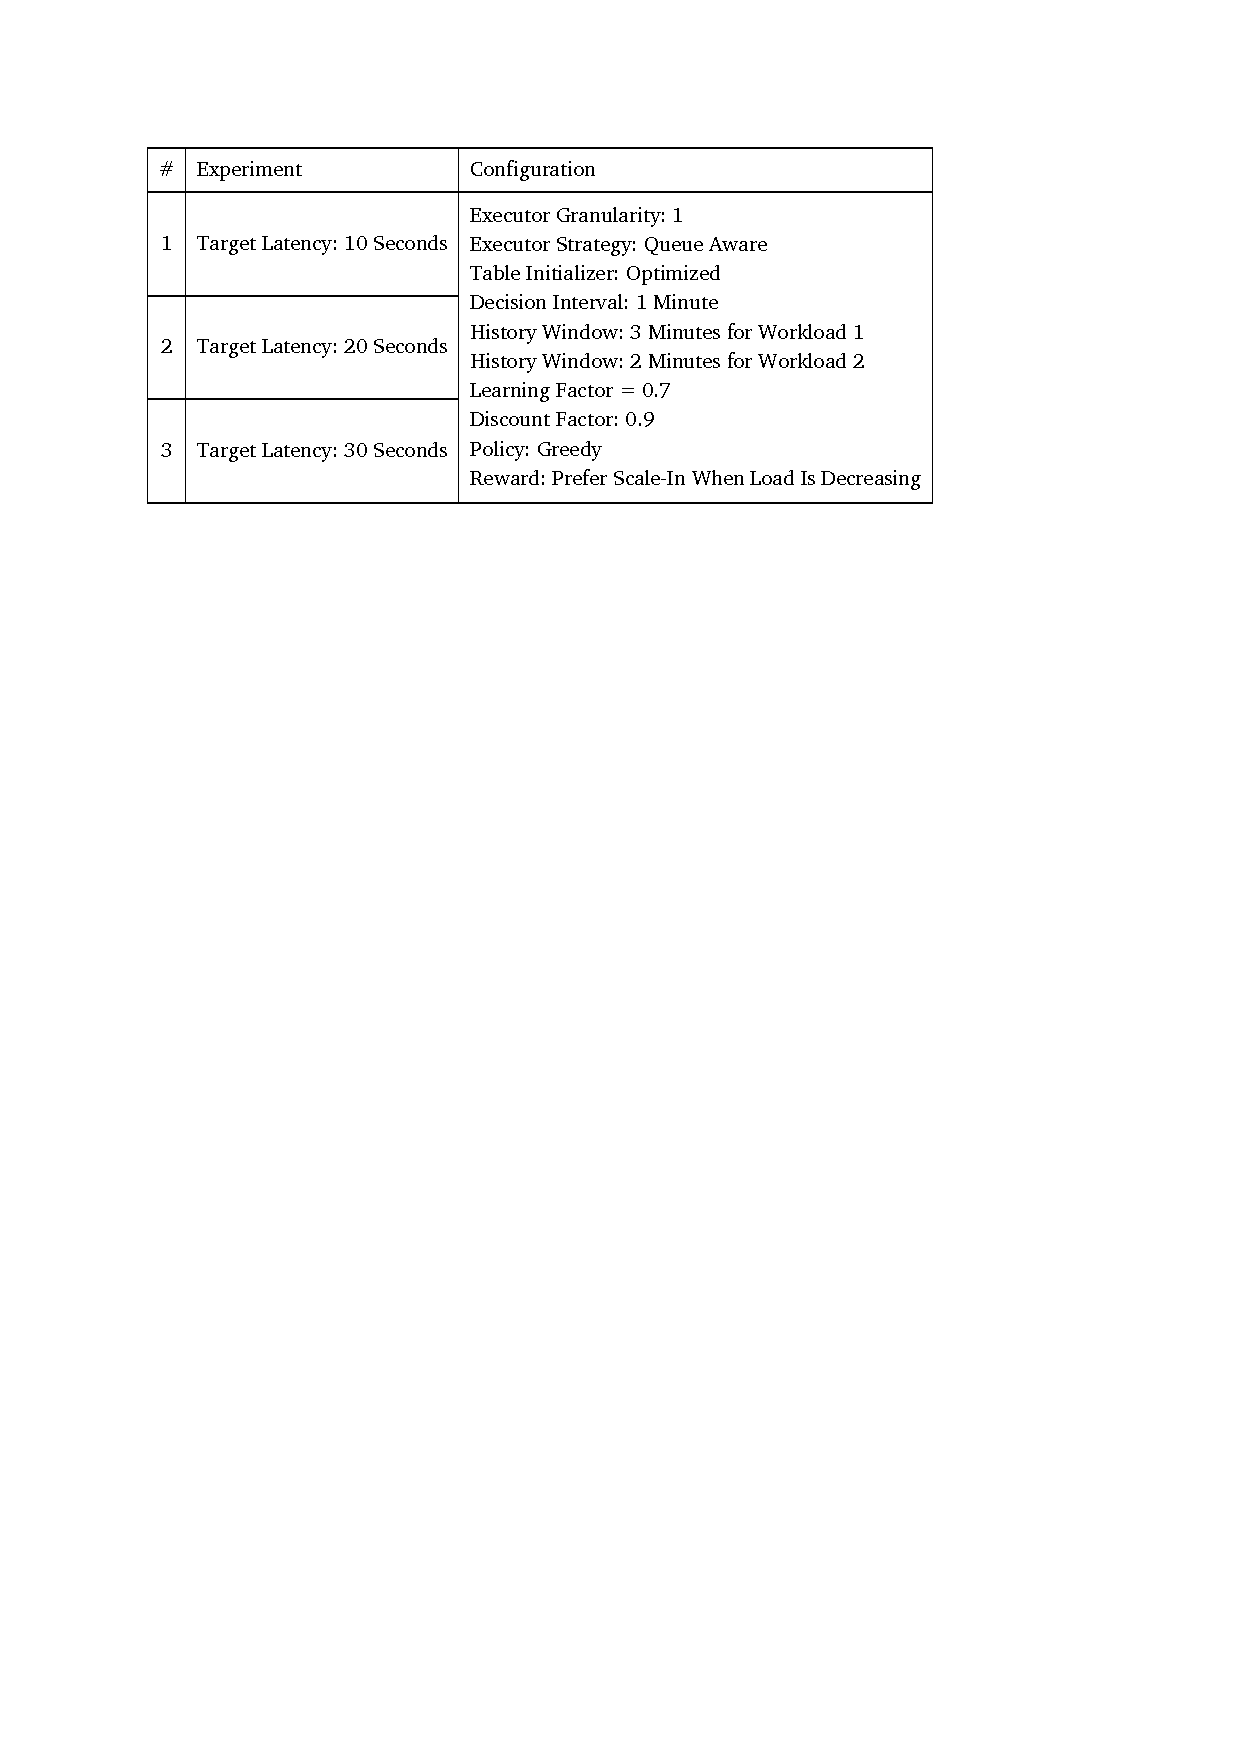
\includegraphics[clip,trim=2.4cm 21.18cm 5.1cm 2.5cm]{tables/ex8.pdf}
    \centering
    \caption{Approaching Target Configuration Parameters}
    \label{eval:tab:ex8}
\end{table}

Figures~\ref{eval:f:e8:w1:lat},~\ref{eval:f:e8:w1:lat-c},~\ref{eval:f:e8:w1:exec} and ~\ref{eval:f:e8:w1:exec-c} illustrates latency and executor charts for Workload 1. Figures~\ref{eval:f:e8:w2:lat},~\ref{eval:f:e8:w2:lat-c},~\ref{eval:f:e8:w2:exec} and~\ref{eval:f:e8:w2:exec-c} illustrates latency and executor charts for Workload 2.

\begin{figure}[!htbp]
    \centering
    \begin{gnuplot}[terminal=epslatex, terminaloptions=color colortext]
        set terminal epslatex size 16cm,7.5cm
        set key outside center top horizontal
        set datafile separator ';'
        set xdata time
        set timefmt '%H:%M:%S'
        set xr ['0:00:00':'1:00:00']
        set yr [0:100]
        set xtics '00:00:00',600 nomirror
        set ytics 0,20 nomirror
        set y2r [0:100]
        set y2tics 0,20 nomirror
        set samples 50000 
        unset mxtics
        unset mytics
        set grid ytics lc rgb "#bbbbbb" lw 1 lt 0
        set grid xtics lc rgb "#bbbbbb" lw 1 lt 0
        unset xl
        set yl 'Latency (Seconds)'
        plot 'ex/e8/w1/latency.csv' using 1:2 w l lc 'red' lw 4 smooth csplines t '10 Sec',\
        '' using 1:3 w l lc 'blue' lw 4 smooth csplines t '20 Sec',\
        '' using 1:4 w l lc 'black' lw 4 smooth csplines t '30 Sec'
    \end{gnuplot}
    \caption{Approaching Target -- Workload 1 -- Latency}
    \label{eval:f:e8:w1:lat}
\end{figure}
\begin{figure}[!htbp]
    \centering
    \begin{minipage}[h]{\linewidth}
        \centering
        \begin{gnuplot}[terminal=epslatex, terminaloptions=color colortext]
            set terminal epslatex size 16cm,7.5cm
            set key outside center top horizontal
            set datafile separator ';'
            set xr [0.5:3.5]
            set yr [0:100]
            set ytics 0,10 nomirror
            set y2r [0:100]
            set y2tics 0,10 nomirror
            set boxwidth 0.3 absolute
            set style fill empty
            set grid ytics lc rgb "#bbbbbb" lw 1 lt 0
            set grid xtics lc rgb "#bbbbbb" lw 1 lt 0
            unset xl
            set yl 'Latency (Seconds)'
            plot 'ex/e8/w1/latency-c.csv' using 1:2:3:4:5:xticlabels(7) with candlesticks lc 'black' lw 4 t 'Min/Max/Percentiles',\
            '' using 1:6:6:6:6 with linespoints pt 5 lc 'black' lw 4 t 'Average'
        \end{gnuplot}
        \caption{Approaching Target -- Workload 1 -- Latency}
        \label{eval:f:e8:w1:lat-c}
    \end{minipage}\hfil
    \begin{minipage}[h]{\linewidth}
        \centering
        \begin{gnuplot}[terminal=epslatex, terminaloptions=color colortext]
            set terminal epslatex size 16cm,7.5cm
            set key outside center top horizontal
            set datafile separator ';'
            set xdata time
            set timefmt '%H:%M:%S'
            set xr ['0:00:00':'1:00:00']
            set yr [2:26]
            set y2r [2:26]
            set ytics 0,4 nomirror
            set xtics '00:00:00',600 nomirror
            set y2tics 0,4 nomirror
            unset mxtics
            unset mytics
            set grid ytics lc rgb "#bbbbbb" lw 1 lt 0
            set grid xtics lc rgb "#bbbbbb" lw 1 lt 0
            unset xl
            set yl 'Number of Executors'
            plot 'ex/e8/w1/exec.csv' using 1:2 w l lc 'red' lw 4 t '5 Min',\
            '' using 1:3 w l lc 'blue' lw 4 t '10 Min',\
            '' using 1:4 w l lc 'black' lw 4 t '20 Min'
        \end{gnuplot}
        \caption{Approaching Target -- Workload 1 -- Number of Executors}
        \label{eval:f:e8:w1:exec}
    \end{minipage}\hfil
    \begin{minipage}[h]{\linewidth}
        \centering
        \begin{gnuplot}[terminal=epslatex, terminaloptions=color colortext]
            set terminal epslatex size 16cm,7.5cm
            set key outside center top horizontal
            set datafile separator ';'
            set xr [0.5:3.5]
            set yr [2:26]
            set y2r [2:26]
            set ytics 0,4 nomirror
            set y2tics 0,4 nomirror
            set boxwidth 0.3 absolute
            set style fill empty
            unset xl
            set grid ytics lc rgb "#bbbbbb" lw 1 lt 0
            set grid xtics lc rgb "#bbbbbb" lw 1 lt 0
            set yl 'Number of Executors'
            plot 'ex/e8/w1/exec-c.csv' using 1:2:3:4:5:xticlabels(7) with candlesticks lc 'black' lw 4 t 'Min/Max/Percentiles',\
            '' using 1:6:6:6:6 with linespoints pt 5 lc 'black' lw 4 t 'Average' 
        \end{gnuplot}
        \caption{Approaching Target -- Workload 1 -- Number of Executors}
        \label{eval:f:e8:w1:exec-c}
    \end{minipage}
\end{figure}
\begin{figure}[!htbp]
    \centering
    \begin{minipage}[h]{\linewidth}
        \centering
        \begin{gnuplot}[terminal=epslatex, terminaloptions=color colortext]
            set terminal epslatex size 16cm,7.5cm
            set key outside center top horizontal
            set datafile separator ';'
            set xdata time
            set timefmt '%H:%M:%S'
            set xr ['0:00:00':'1:00:00']
            set yr [0:110]
            set y2r [0:110]
            set xtics '00:00:00',600 nomirror
            set ytics 0,20 nomirror
            set y2tics 0,20 nomirror
            unset mxtics
            unset mytics
            set samples 50000 
            unset xl
            set grid ytics lc rgb "#bbbbbb" lw 1 lt 0
            set grid xtics lc rgb "#bbbbbb" lw 1 lt 0
            set yl 'Latency (Seconds)'
            plot 'ex/e8/w2/latency.csv' using 1:2 w l lc 'red' lw 4 smooth csplines t '10 Sec',\
            '' using 1:3 w l lc 'blue' lw 4 smooth csplines t '20 Sec',\
            '' using 1:4 w l lc 'black' lw 4 smooth csplines t '30 Sec'
        \end{gnuplot}
        \caption{Approaching Target -- Workload 2 -- Latency}
        \label{eval:f:e8:w2:lat}
    \end{minipage}\hfil
    \begin{minipage}[h]{\linewidth}
        \centering
        \begin{gnuplot}[terminal=epslatex, terminaloptions=color colortext]
            set terminal epslatex size 16cm,7.5cm
            set key outside center top horizontal
            set datafile separator ';'
            set xr [0.5:3.5]
            set yr [0:110]
            set y2r [0:110]
            set ytics 0,10 nomirror
            set y2tics 0,10 nomirror
            set boxwidth 0.3 absolute
            set style fill empty
            unset xl
            set grid ytics lc rgb "#bbbbbb" lw 1 lt 0
            set grid xtics lc rgb "#bbbbbb" lw 1 lt 0            
            set yl 'Latency (Seconds)'
            plot 'ex/e8/w2/latency-c.csv' using 1:2:3:4:5:xticlabels(7) with candlesticks lc 'black' lw 4 t 'Min/Max/Percentiles',\
            '' using 1:6:6:6:6 with linespoints pt 5 lc 'black' lw 4 t 'Average'
        \end{gnuplot}
        \caption{Approaching Target -- Workload 2 -- Latency}
        \label{eval:f:e8:w2:lat-c}
    \end{minipage}\hfil
    \begin{minipage}[h]{\linewidth}
        \centering
        \begin{gnuplot}[terminal=epslatex, terminaloptions=color colortext]
            set terminal epslatex size 16cm,7.5cm
            set key outside center top horizontal
            set datafile separator ';'
            set xdata time
            set timefmt '%H:%M:%S'
            set xr ['0:00:00':'1:00:00']
            set yr [2:26]
            set y2r [2:26]
            set xtics '00:00:00',600 nomirror
            set ytics 0,4 nomirror
            set y2tics 0,4 nomirror
            unset mxtics
            unset mytics
            unset xl
            set grid ytics lc rgb "#bbbbbb" lw 1 lt 0
            set grid xtics lc rgb "#bbbbbb" lw 1 lt 0     
            set yl 'Number of Executors'
            plot 'ex/e8/w2/exec.csv' using 1:2 w l lc 'red' lw 4 t '10 Sec',\
            '' using 1:3 w l lc 'blue' lw 4 t '20 Sec',\
            '' using 1:4 w l lc 'black' lw 4 t '30 Sec'
        \end{gnuplot}
        \caption{Approaching Target -- Workload 2 -- Number of Executors}
        \label{eval:f:e8:w2:exec}
    \end{minipage}
\end{figure}
\begin{figure}[!htbp]
    \centering
    \begin{gnuplot}[terminal=epslatex, terminaloptions=color colortext]
        set terminal epslatex size 16cm,7.5cm
        set key outside center top horizontal
        set datafile separator ';'
        set xr [0.5:3.5]
        set yr [2:26]
        set ytics 0,4 nomirror
        set y2r [2:26]
        set y2tics 0,4 nomirror
        set boxwidth 0.3 absolute
        set style fill empty
        unset xl
        set grid ytics lc rgb "#bbbbbb" lw 1 lt 0
        set grid xtics lc rgb "#bbbbbb" lw 1 lt 0  
        set yl 'Number of Executors'
        plot 'ex/e8/w2/exec-c.csv' using 1:2:3:4:5:xticlabels(7) with candlesticks lc 'black' lw 4 t 'Min/Max/Percentiles','' using 1:6:6:6:6 with linespoints pt 5 lc 'black' lw 4 t 'Average' 
    \end{gnuplot}
    \caption{Approaching Target -- Workload 2 -- Number of Executors}
    \label{eval:f:e8:w2:exec-c}
\end{figure}
\FloatBarrier
\subsection{Conclusion}
Looking at results, the more we get close to 10-second target latency, the more it gets challenging for Auto-Scaler. However, there is one common behavior in both workloads. The key factor to reduce latency is to apply \emph{early} Scale-Out. This can be confirmed by Figure~\ref{eval:f:e8:w1:exec} and Figure~\ref{eval:f:e8:w2:exec}. However, as explained in Section~\ref{intro-auto-scale}, Reinforcement Learning agent has to visit a state to take an appropriate action which may be too late when the peak workload is observed. This is one of the cases where proactive -- predictive -- approaches are more useful.
\clearpage
\section{Experiment 9: Overall Comparison}
In this experiment implemented Q-Learning technique is compared to bare bone Spark with fixed number of executors and Spark Streaming's default dynamic resource manager. Furthermore, Online Parameter Optimization~\cite{Heinze:2015} which is implemented for Spark Streaming by~\textcite{Michal:2017} is also included. Table~\ref{eval:tab:ex9} describes the configuration parameters of this experiment.
\begin{table}[h]
    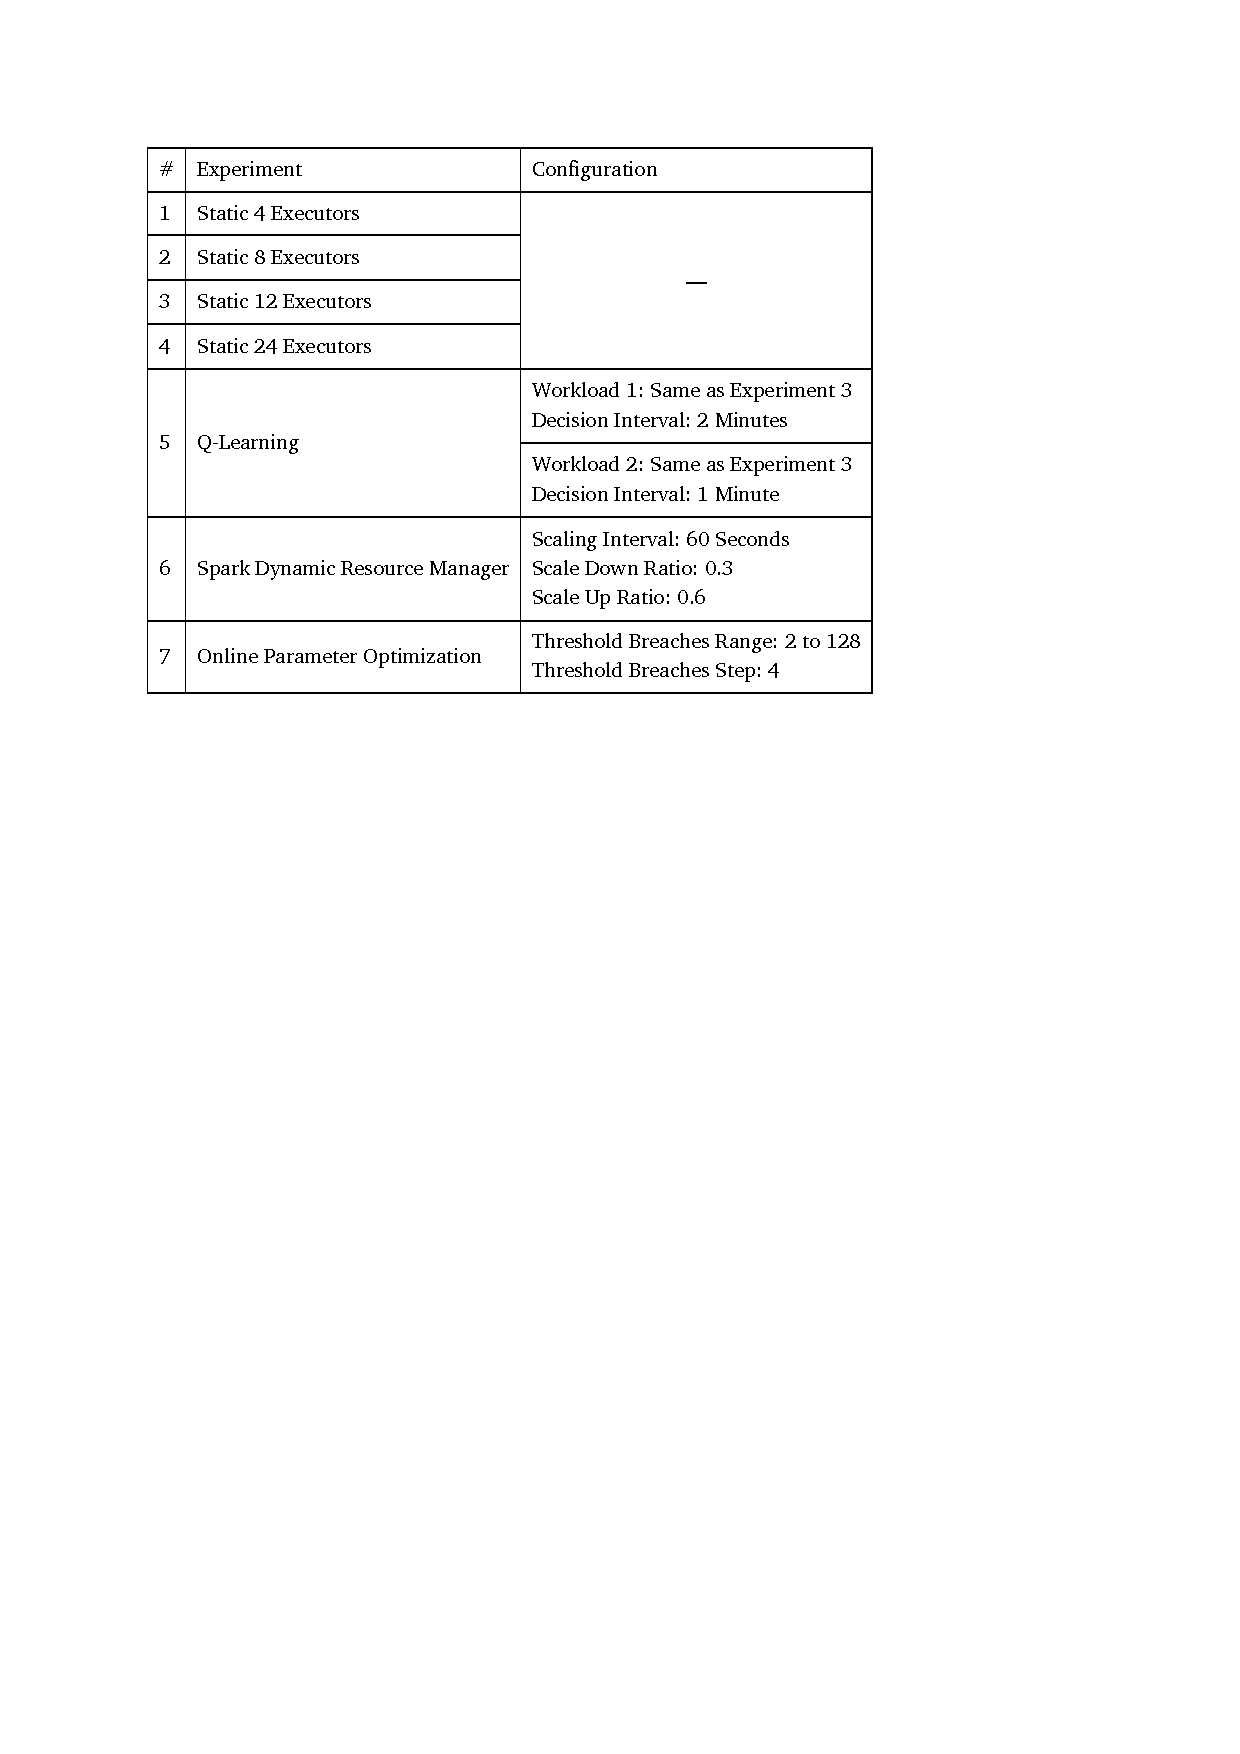
\includegraphics[clip,trim=2.4cm 17.9cm 6.1cm 2.5cm]{tables/ex9.pdf}
    \centering
    \caption{Overall Comparison Configuration Parameters}
    \label{eval:tab:ex9}
\end{table}

Note that, Spark Dynamic Resource Manager uses Equation~\ref{eval:e9:formula} to calculate a \emph{Ratio} value and then compares it to Scale-Up and Scale-Down ratio values obtained from configuration. In order to influence the behavior of this resource manager, batch duration should be changed. To make it fair, in all experiments the batch size is set to 10 seconds.
\begin{equation}
\text{Ratio} = \frac{\text{Average Latency of History Window}}{\text{Batch Size}}
\label{eval:e9:formula}
\end{equation}

For Q-Learning approach, two of the best cases from previous experiments were obtained. Also note that seven cases are evaluated in this experiment which makes it difficult to comprehend the detailed latency charts. Thus, they are removed. Figures~\ref{eval:f:e9:w1:lat-c} and~\ref{eval:f:e9:w2:lat-c} illustrate latency charts for both workloads. Figures~\ref{eval:f:e9:w1:exec-c} and~\ref{eval:f:e9:w2:exec-c} illustrates executor charts for both workloads.

\begin{figure}[!htbp]
    \centering
    \begin{minipage}[h]{\linewidth}
        \centering
        \begin{gnuplot}[terminal=epslatex, terminaloptions=color colortext]
            set terminal epslatex size 17cm,11cm
            set key outside center top horizontal
            set datafile separator ';'
            set xr [0.5:7.5]
            set yr [0:420]
            set ytics 0,30 nomirror
            set y2r [0:420]
            set y2tics 0,30 nomirror
            set boxwidth 0.4 absolute
            set style fill empty
            set grid ytics lc rgb "#bbbbbb" lw 1 lt 0
            set grid xtics lc rgb "#bbbbbb" lw 1 lt 0
            unset xl
            set yl 'Latency (Seconds)'
            plot 'ex/final/w1/latency-c.csv' using 1:2:3:4:5:xticlabels(7) with candlesticks lc 'black' lw 4 t 'Min/Max/Percentiles',\
            '' using 1:6:6:6:6 with linespoints pt 5 lc 'black' lw 4 t 'Average'
        \end{gnuplot}
        \caption{Overall Comparison -- Workload 1 -- Latency}
        \label{eval:f:e9:w1:lat-c}
    \end{minipage}\hfil
    \begin{minipage}[h]{\linewidth}
        \centering
        \begin{gnuplot}[terminal=epslatex, terminaloptions=color colortext]
            set terminal epslatex size 17cm,11cm
            set key outside center top horizontal
            set datafile separator ';'
            set xr [0.5:7.5]
            set yr [0:390]
            set ytics 0,30 nomirror
            set y2r [0:390]
            set y2tics 0,30 nomirror
            set boxwidth 0.4 absolute
            set style fill empty
            set grid ytics lc rgb "#bbbbbb" lw 1 lt 0
            set grid xtics lc rgb "#bbbbbb" lw 1 lt 0
            unset xl
            set yl 'Latency (Seconds)'
            plot 'ex/final/w2/latency-c.csv' using 1:2:3:4:5:xticlabels(7) with candlesticks lc 'black' lw 4 t 'Min/Max/Percentiles',\
            '' using 1:6:6:6:6 with linespoints pt 5 lc 'black' lw 4 t 'Average'
        \end{gnuplot}
        \caption{Overall Comparison -- Workload 2 -- Latency}
        \label{eval:f:e9:w2:lat-c}
    \end{minipage}
\end{figure}
\begin{figure}[!h]
    \centering
    \begin{minipage}[h]{\linewidth}
    \centering
    \begin{gnuplot}[terminal=epslatex, terminaloptions=color colortext]
        set terminal epslatex size 16cm,7.5cm
        set key outside center top horizontal
        set datafile separator ';'
        set xr [0.5:7.5]
        set yr [2:26]
        set y2r [2:26]
        set ytics 0,4 nomirror
        set y2tics 0,4 nomirror
        set boxwidth 0.4 absolute
        set style fill empty
        unset xl
        set grid ytics lc rgb "#bbbbbb" lw 1 lt 0
        set grid xtics lc rgb "#bbbbbb" lw 1 lt 0
        set yl 'Number of Executors'
        plot 'ex/final/w1/exec-c.csv' using 1:2:3:4:5:xticlabels(7) with candlesticks lc 'black' lw 4 t 'Min/Max/Percentiles',\
        '' using 1:6:6:6:6 with linespoints pt 5 lc 'black' lw 4 t 'Average' 
    \end{gnuplot}
    \caption{Overall Comparison -- Workload 1 -- Number of Executors}
    \label{eval:f:e9:w1:exec-c}
    \end{minipage}\hfil
    \begin{minipage}[h]{\linewidth}
    \centering
    \begin{gnuplot}[terminal=epslatex, terminaloptions=color colortext]
        set terminal epslatex size 16cm,7.5cm
        set key outside center top horizontal
        set datafile separator ';'
        set xr [0.5:7.5]
        set yr [2:26]
        set y2r [2:26]
        set ytics 0,4 nomirror
        set y2tics 0,4 nomirror
        set boxwidth 0.4 absolute
        set style fill empty
        unset xl
        set grid ytics lc rgb "#bbbbbb" lw 1 lt 0
        set grid xtics lc rgb "#bbbbbb" lw 1 lt 0
        set yl 'Number of Executors'
        plot 'ex/final/w2/exec-c.csv' using 1:2:3:4:5:xticlabels(7) with candlesticks lc 'black' lw 4 t 'Min/Max/Percentiles',\
        '' using 1:6:6:6:6 with linespoints pt 5 lc 'black' lw 4 t 'Average' 
    \end{gnuplot}
    \caption{Overall Comparison -- Workload 2 -- Number of Executors}
    \label{eval:f:e9:w2:exec-c}
    \end{minipage}
\end{figure}
\subsection{Conclusion}
As can be seen, from 8 to 12 executors the latency drops significantly. It can be concluded that to hit target latency -- which is 30 seconds in this case -- optimal number of executors is between 8 to 12. Note that, 12 executors is slightly better than 24 executors. This could be the result of extra network communication involved in case of 24 executors. Spark and OPO achieve better latency than Q-Learning approach but with much more executors.
\chapter{Related Work}
\label{related}
Dynamic resource allocation in cloud environments has been studied extensively in literature. In this chapter prior work will be discussed and explored. It is organized as follows. Section~\ref{related:thb} delves into threshold-based techniques. Section~\ref{related:tsa} investigates techniques based on time-series analysis. Section~\ref{related:qt} analyses techniques based on queuing theory. Section~\ref{related:rl} explores Reinforcement Learning techniques comprehensively. Finally, section~\ref{related:sum} concludes.

\section{Threshold-Based Techniques}
\label{related:thb}

\textcite{Hasan2012IntegratedAA} proposed four thresholds and two time periods. \lstinline$ThrUpper$ defines upper bound. \lstinline$ThrBelowUpper$ is slightly below \lstinline$ThrUpper$. Similarly, \lstinline$ThrLower$ defines lower bound and \lstinline$ThrAboveLower$ is slightly above the lower bound. In case, system utilization stays between \lstinline$ThrUpper$ and \lstinline$ThrBelowUpper$ for a specific duration, then cluster controller decides to take a scale-out action, by adding resources. On the other hand, if system utilization stays between \lstinline$ThrLower$ and \lstinline$ThrAboveLower$ for a specified duration, then the central controller decides to take scale-in action. Furthermore, in order to prevent making \emph{oscillating} decisions, \emph{grace period} is enforced. During this period, no scaling decision is made. Defining two levels of thresholds helps to detect workload \emph{persistency} and avoids making immature scaling decision. However, defining thresholds is a tricky and manual process, and needs to be carefully done~\cite{Dutreilh2010}. It shall be noted that, computation overhead of this approach is very low.

\emph{RightScale}~\cite{RightScale} applies voting algorithm among nodes to make scaling decisions. In order for a specific action to be decided, majority of nodes should vote in favor of that specific action. Otherwise, no-action is elected as a default action. Afterwards, nodes apply grace period to stabilize the cluster. The complexity of the voting process in trusted environments is in the order of $O(n^2)$, which leads to heavy network traffic among participants when cluster size grows. This approach also suffers from the same issue -- accurately adjusting threshold values -- as other threshold-based approaches.

\textcite{Heinze:2015} proposed a novel threshold-based solution in the context of FUGU~\cite{Grandl:2014:MPC} -- a data stream processing framework. This techniques uses an adaptive window~\cite{Bifet:2007} to monitor the recent changes in workload pattern. In case a change in workload is detected, optimization component is activated and fed with recent short-term utilization history. Thereafter, the optimization component determines monetary cost of current system configuration and then simulates the cost of different scaling decisions. The \emph{latency-aware} cost function has the responsibility to calculate monetary cost of system configuration. The search function is an implementation of \emph{Recursive Random Search}~\cite{Ye:2003:RRS} algorithm which consists of two phases. First, in \emph{exploration} phase, the complete parameter space is explored to find a solution with minimum cost. In second phase -- \emph{exploitation phase} -- only specific parts of the parameter space which has been discovered in first phase, will be investigated. \textcite{Michal:2017} has implemented this techniques in the context of Spark Streaming. Thus, It is considered in evaluation scenarios.

\section{Time-Series Analysis Techniques}
\label{related:tsa}

\textcite{Herbst:2013} surveys different auto-scaling techniques based on time-series analysis in order to forecast \emph{trends} and \emph{seasons}. \emph{Moving Average Method} takes the average over a sliding window and smooths out minor noise level. Its computational overhead is proportional to size of the window. \emph{Simple Exponential Smoothing}(SES) goes further than just taking average. It gives more weight to more recent values in sliding window by an exponential factor. Although it is more computationally intensive compared to moving average, it is still negligible. SES is capable of detecting short-term trends but fails at predicting seasons. These approaches are more specific instances of \emph{ARIMA} (Auto-Regressive Integrated Moving Average) which is a general purpose framework to calculate moving averages. However, time-series analysis is only suitable for stationary problems consist of recurring workload patterns such as web applications. Additionally, more advanced forms of time-series analysis which are capable of forecasting seasons (such as \emph{tBATS Innovation State Space Modeling Framework}~\cite{Alysha2011}, \emph{ARIMA Stochastic Process Modeling Framework}~\cite{JSSv027i03}) are computationally infeasible for streaming workloads.

\textcite{Taft:2018} applied time-series analysis in the context of OLTP databases. The authors argue that reactive approaches don't fit to database world. By the time, auto-scaler component decides to scale-out, it is already too late for a database system. This premise comes from the fact that taking scaling actions in a database doesn't take place in timely manner. The database system has to replicate some of the records which is an additional burden on a heavily loaded system. Thus, database system must take proactive approach and take scaling decisions ahead of time. While this is convincing argument, the auto-scaler module depends on a couple of parameters that are hard to calculate in heterogeneous public cloud environments. First, target throughput of a single server. Second, shortest time to move all database records with single sender-receiver thread. While this might be feasible in some scenarios, on today's cloud environments with virtual machines hosted on heterogeneous physical nodes, getting a near-precise number is unconvincing. It worth noting that author assumed an approximately uniform workload distribution for all database nodes -- each database shard serves a fairly equal portion of total workload which is a questionable assumption.

\section{Queuing Theory Techniques}
\label{related:qt}

\textcite{Lohrmann:2015} proposed a solution based on queuing theory. The solution is designed for \emph{Nephele}~\cite{Lohrmann:2014} streaming engine which has a master-worker style architecture. Similar to Spark Streaming, a job is modeled as a DAG. It utilizes \emph{adaptive output batching}~\cite{Warneke:2011} -- which is essentially a buffer with variable size -- to buffer outgoing messages emitted from one stage to the other. Each task -- an executer that runs user defined function (UDF) -- is modeled as a G/G/1 queue. That is, the probability distributions of message inter-arrival and service time are unknown. In order to approximate these distributions, a formula proposed by \textcite{Kingman:1961} is used. From a bird's eye view, this solution seems promising. However, authors made two unconvincing assumptions that led us to abandon the proposal. First, worker nodes shall be homogeneous in terms of processing power and network bandwidth. Second, there should be an effective partitioning strategy in place in order to load balance outgoing messages between stages. In reality both assumptions rarely occur. Large scale stream processing clusters are built incrementally. Depending on workload, data skew does exist and imperfect hash functions are widely used by software developers.

\textcite{Zhang:2007} proposed a solution for multi-tiered enterprise applications based on regression techniques. Regression based models can absorb some level of uncertainty and noise by compacting samples. Each tier is modeled as G/G/1 queue and scaled differently compared to other tiers. The system has fixed number of users -- a principle known as \emph{closed-loop queuing network}. In order to calculate system workload -- incoming message rate -- and service time which is required by queuing models, the authors proposed to use Mean Value Analysis~\cite{Menasce:2004}. In order to simplify the queuing network, the system is modeled as a \emph{transaction-based} system with independent requests coming from clients. However, It is widely believed that multi-tiered enterprise applications are \emph{session-based} systems~\cite{Cherkasova:2002}. Each request from the same client depends on her previous request during a specific session.
 
\section{Reinforcement Learning Techniques}
\label{related:rl}

\textcite{Herbst:2017} surveys on state of the art techniques to predict future workload. It includes workload forecasting based on \emph{Bayesian Networks} (BN) and \emph{Neural Networks}. There are several issues with each of them that makes them unsuitable for streaming workloads. As an example, there is no universally applicable method to construct a BN. Furthermore, it requires collecting data and training the model offline. Neural networks suffer from the same issues. That is, it requires collecting samples and periodically training the model. For complex models, training phase is typically computationally infeasible which is conflicting with requirements of thesis.

\textcite{Tesauro2006} proposes a hybrid approach to overcome poor performance of online training. The system consists of two components: an online component based on queuing system combined with Reinforcement Learning component that is trained offline. The offline component is based on \emph{neural networks}. The authors model the data center as multiple applications managed under a single resource manager. Modeling streaming workloads as a queuing system has two problems. First, modeling is a complicated process and determining probability distributions requires domain knowledge. Second, it requires access to each node (so it can be modeled as a queue) which is currently not possible without modifying \lstinline$spark-core$ package. Since, it was one the requirements to provide a solution without making any modification to \lstinline$spark-core$, this work has been abandoned.

\textcite{Rao:2009:VRL} proposed to use Reinforcement Learning to manage resources consumed by virtual machines. It employs standard model-free learning, which is known as \emph{Temporal Difference}~\cite{rlIntro} or \emph{Sarsa} algorithm. The state space consists of metrics collected from virtual machines (CPU, RAM, Network IO, \dots). There is no global controller and each node decides based on its own Q-Table. As mentioned in literature, standard temporal difference has a slow convergence speed. In order to speedup bootstrap phase, Q-Table is initialized by values that were obtained during separate supervised training. Since this approach also relies on offline training, it wasn't adopted by this thesis.

\textcite{Enda:2012} proposed a parallel architecture to Reinforcement Learning. Standard model-free learning (Temporal Difference) is used. No global controller is involved and each node decides locally. In order to speed up learning, all nodes maintain two Q-Tables (local and global tables). Local table is learned and updated by each node. Whenever, an agent learns a new value for a specific state, it broadcasts it to other agents. The global table contains values received from other agents. Additionally, agent prioritize local and global tables by assigning weights to each table. Weights are factors that are defined by application developers. The final decision is the outcome of combining local and global tables. Although each node learns some part of the state space (which may overlap with other nodes), it is not applicable in the context of Spark Streaming. The assumption in this architecture is that, each node is operating autonomously without intervention from other nodes (such as web servers). In contrast, Spark is a centrally managed system. That is, all nodes running Spark jobs are supervised by a single master node (probably with couple of backup masters).

\textcite{Heinze:2014} implemented Reinforcement Learning in the context of FUGU~\cite{Grandl:2014:MPC} and compared it to threshold-based approaches. Each node, maintains its own Q-Table and imposes local policy without coordinating other nodes. This architecture can not be applied in the context of spark streaming, since Spark abstracts away individual nodes from the perspective of application developer. In order to decrease state space, the author applied two techniques. First, only system utilization is considered. Second, system utilization is discretized using coarse grained steps. To remedy slow convergence, the controller enforces a \emph{monotonicity constraint}~\cite{Herodotou:2011}. That is, if the controller decides to take scale-out action for a specific utilization, it may not decide scale-in for even worse system utilization. This feature has been adopted by this thesis.  

\textcite{CARDELLINI2018171} proposed a two level hierarchical architecture for resource management in Apache Storm~\cite{Storm}. There is a local controller on each node which is cooperating with the global controller. The local controller monitors each operator using different policies (threshold-based or Reinforcement Learning using temporal difference). In case, local controller decides to scale in or out an specific operator, it contacts the global controller and informs it about its decision. Then it waits to receive confirmation from the global controller. The global controller operates using a token-bucket-based policy~\cite{Valeria:2018} and has global view of cluster. It ranks requests coming from local controllers and either confirms or rejects their decisions. Although, this architecture seems to be a promising approach, however it has been implemented by modifying Storm's internal components. As mentioned above, this is in conflict with thesis's requirements.

In order to mitigate the problem of large state space in Reinforcement Learning, \textcite{Lolos:2017} proposed to start the agent from small number of coarse grained states. As more metrics are collected (and stored as historical records), agent will discover \emph{outlier} parameters (those parameters that are affecting agent more, CPU rather than IO as an example). Then, it partitions the affected state into two states and \emph{re-trains} newly added states using historical records. Both Temporal Difference and Value Iteration methods can be used as learning algorithm. Gradually, agent only focuses on some specific parts of the state space, since all parameters are not equally important. This approach, effectively reduces the size of state space. However, the trade-off is the storage cost in which historical metrics need to be stored. It worth noting that from the context of paper, storage cost (whether it is in-memory or on-disk and the duration of storing historical metrics) is unclear. Thus, this approach has been abandoned due to uncertainty.

\textcite{dutreilh:hal-01122123} proposed a model-based Reinforcement Learning approach for resource management of cloud applications. All virtual machines are supervised by a single global controller. Slow convergence is the bottleneck of model-free learning, in contrast to model-based learning. However, environment dynamics are not available at the time of modeling. Authors proposed to estimate these parameters as more metrics are collected and then switch to \emph{Value Iteration}~\cite{rlIntro} algorithm instead of \emph{Temporal Difference}. In short, statistical metrics are stored and updated for each visit of (old state, action, reward, new state) quadruple. As more samples are collected, statistical metrics become more accurate and can be directly used in \emph{Bellman} equation. Until enough measurements get collected, a separate initial reward function is used which is essentially the original reward function but with penalty costs removed. Furthermore, In order to reduce the state space -- tuple of [request/sec, number of VMs, average response time] -- there exists a predefined upper and lower bound for state variables and average response time is measured at granularity of seconds. This approach has been partially adopted by this thesis.

\textcite{Dutreilh2010} proposed a model-free Reinforcement Learning approach (\emph{Temporal difference} algorithm) with modified \emph{exploration} policy. The standard exploration policy for Q-Learning is $1-\epsilon$. Under this policy, the agent performs a random action with probably of $\epsilon$ and with probability of $1-\epsilon$, it adheres to an action proposed by optimal policy. Although the random action is necessary to explore unknown states, but it has sever consequences under streaming workloads. In some cases, it leads to unsafe states where SLOs are severely violated. Since streaming is heavily latency sensitive, this property is undesirable. Thus, author sought toward a heuristic-based policy proposed by~\textcite{Bodik:2009}. This policy is based on couple of key observations which has been adopted by this thesis:
\begin{itemize}
    \item It must quickly explore different states.
    \item It should collect accurate data as fast as possible, to speedup training.
    \item During exploration phase, the policy should be careful not to violate SLOs.
\end{itemize}

\section{Summary}
\label{related:sum}

In this chapter prior work on auto-scaling scaling has been discussed and evaluated. First, threshold-based approaches are investigated. Simple threshold-based approaches are intuitive and simple to understand by application developers and are widely supported by cloud providers. However, adjusting thresholds is a tricky and error-prone process. Then, time-series analysis techniques are explored. As confirmed by other authors, advanced seasonal forecasting is a computationally intensive process, which makes it less suitable for streaming workloads. Queuing theory approaches are suitable for stationary networks with a known probability distribution for workload and service time. Reinforcement Learning techniques has the benefit that it requires zero knowledge about the environment which helps to gradually adapt to changes in environment.
\chapter{Conclusion}
\label{conc}

\newpage

\pagenumbering{Roman}
\setcounter{page}{\value{romanpagenumbers}}

\printbibliography

\end{document}  